\documentclass[11pt,a4paper]{article}
\usepackage[T1]{fontenc}
\usepackage[utf8]{inputenc}
\usepackage{mathpazo}
\renewcommand{\ttdefault}{txtt}
\linespread{1.06}
\usepackage[margin=2.2cm,headheight=14pt]{geometry}
\usepackage{microtype}
\usepackage{amsmath,amssymb,mathtools,bm}
\usepackage{xcolor}
\usepackage{colortbl}
\usepackage{graphicx}
\usepackage{booktabs,tabularx,longtable,array,multirow}
\usepackage{enumitem}
\usepackage{siunitx}
\usepackage{listings}
\usepackage[most]{tcolorbox}
\usepackage{tikz}
\usetikzlibrary{arrows.meta,positioning,calc,shapes.geometric,decorations.pathreplacing,fit,backgrounds,matrix,patterns}
\usepackage{pgfplots}
\pgfplotsset{compat=1.18}
\usepackage{fancyhdr}
\usepackage{titlesec}
\usepackage[hidelinks]{hyperref}
\usepackage[nameinlink,capitalise]{cleveref}

% ---------- colours ----------
\definecolor{ink}{HTML}{1F2933}
\definecolor{idea}{HTML}{2B6CB0}
\definecolor{repo}{HTML}{2F855A}
\definecolor{warn}{HTML}{C05621}
\definecolor{shapec}{HTML}{6B46C1}
\definecolor{cIn}{HTML}{E2E8F0}
\definecolor{c16}{HTML}{BEE3F8}
\definecolor{c32}{HTML}{C6F6D5}
\definecolor{c64}{HTML}{FED7D7}
\definecolor{cK}{HTML}{FEEBC8}
\definecolor{cG}{HTML}{E9D8FD}
\definecolor{codebg}{HTML}{F7FAFC}
\color{ink}

% ---------- headers ----------
\pagestyle{fancy}
\fancyhf{}
\fancyhead[L]{\small\textsc{ResNet-20 refresher}}
\fancyhead[R]{\small\nouppercase{\rightmark}}
\fancyfoot[C]{\small\thepage}
\renewcommand{\headrulewidth}{0.3pt}
\titleformat{\section}{\Large\bfseries\color{idea!70!black}}{\thesection}{0.8em}{}
\titleformat{\subsection}{\large\bfseries}{\thesubsection}{0.7em}{}
\setlength{\parindent}{0pt}
\setlength{\parskip}{0.55em}

% ---------- boxes ----------
\newtcolorbox{idea}[1][]{enhanced,breakable,colback=idea!4,colframe=idea,boxrule=0.6pt,arc=2pt,left=6pt,right=6pt,top=9pt,bottom=5pt,
  fonttitle=\bfseries\small,title={General idea\ifx&#1&\else: #1\fi},attach boxed title to top left={xshift=6pt,yshift=-2mm},boxed title style={colback=idea,arc=1pt,boxrule=0pt}}
\newtcolorbox{repo}[1][]{enhanced,breakable,colback=repo!4,colframe=repo,boxrule=0.6pt,arc=2pt,left=6pt,right=6pt,top=9pt,bottom=5pt,
  fonttitle=\bfseries\small,title={In this repository\ifx&#1&\else: #1\fi},attach boxed title to top left={xshift=6pt,yshift=-2mm},boxed title style={colback=repo,arc=1pt,boxrule=0pt}}
\newtcolorbox{warn}[1][]{enhanced,breakable,colback=warn!5,colframe=warn,boxrule=0.6pt,arc=2pt,left=6pt,right=6pt,top=9pt,bottom=5pt,
  fonttitle=\bfseries\small,title={Detail / deviation\ifx&#1&\else: #1\fi},attach boxed title to top left={xshift=6pt,yshift=-2mm},boxed title style={colback=warn,arc=1pt,boxrule=0pt}}
\newtcolorbox{shapebox}[1][]{enhanced,breakable,colback=shapec!4,colframe=shapec,boxrule=0.6pt,arc=2pt,left=6pt,right=6pt,top=9pt,bottom=5pt,
  fonttitle=\bfseries\small,title={Shape check\ifx&#1&\else: #1\fi},attach boxed title to top left={xshift=6pt,yshift=-2mm},boxed title style={colback=shapec,arc=1pt,boxrule=0pt}}

% ---------- code ----------
\lstset{basicstyle=\ttfamily\footnotesize,backgroundcolor=\color{codebg},frame=single,rulecolor=\color{black!15},
  keywordstyle=\color{idea}\bfseries,commentstyle=\color{black!50}\itshape,stringstyle=\color{repo!80!black},
  showstringspaces=false,columns=fullflexible,keepspaces=true,breaklines=true,xleftmargin=4pt,xrightmargin=4pt,language=Python,
  numbers=left,numberstyle=\tiny\color{black!40},numbersep=6pt}
\newcommand{\code}[1]{\texttt{#1}}
\newcommand{\file}[1]{\textcolor{repo!80!black}{\texttt{#1}}}

% ---------- maths shortcuts ----------
\newcommand{\R}{\mathbb{R}}
\newcommand{\shp}[1]{\textcolor{shapec}{\ensuremath{(#1)}}}
\newcommand{\T}{^{\!\top}}
\DeclareMathOperator*{\argmax}{arg\,max}
\DeclareMathOperator{\ReLU}{ReLU}
\DeclareMathOperator{\BN}{BN}
\DeclareMathOperator{\softmax}{softmax}
\DeclareMathOperator{\conv}{conv}
\newcommand{\dd}[2]{\frac{\partial #1}{\partial #2}}

% ---------- TikZ drawing helpers ----------
% \tensor{x}{y}{W}{H}{D}{fill}{wlabel}{hlabel}{dlabel}   (front face lower-left at (x,y); depth drawn up-right)
\newcommand{\tensor}[9]{%
  \begin{scope}[shift={(#1,#2)}]
    \colorlet{tfill}{#6}%
    \pgfmathsetmacro{\dx}{0.55*#5}\pgfmathsetmacro{\dy}{0.40*#5}
    \fill[tfill!90!black] (0,#4) -- ++(\dx,\dy) -- ++(#3,0) -- ++(-\dx,-\dy) -- cycle;
    \fill[tfill!78!black] (#3,0) -- ++(\dx,\dy) -- ++(0,#4) -- ++(-\dx,-\dy) -- cycle;
    \fill[tfill] (0,0) rectangle (#3,#4);
    \draw[ink,line width=0.5pt] (0,0) rectangle (#3,#4);
    \draw[ink,line width=0.5pt] (0,#4) -- ++(\dx,\dy) -- ++(#3,0) -- ++(0,-#4) -- ++(-\dx,-\dy);
    \draw[ink,line width=0.5pt] (#3,#4) -- ++(\dx,\dy);
    \node[below,font=\scriptsize] at (#3/2,0) {#7};
    \node[left,font=\scriptsize] at (0,#4/2) {#8};
    \node[above left,font=\scriptsize,inner sep=1pt] at (\dx/2,#4+\dy/2) {#9};
  \end{scope}}
% \matr{x}{y}{W}{H}{fill}{name}{rows}{cols}
\newcommand{\matr}[8]{%
  \begin{scope}[shift={(#1,#2)}]
    \fill[#5] (0,0) rectangle (#3,#4);
    \draw[ink,line width=0.5pt] (0,0) rectangle (#3,#4);
    \node[font=\small] at (#3/2,#4/2) {#6};
    \node[left,font=\scriptsize] at (0,#4/2) {#7};
    \node[above,font=\scriptsize] at (#3/2,#4) {#8};
  \end{scope}}

\usepackage{cancel}
\begin{document}
\begin{titlepage}
\centering
\vspace*{2.2cm}
{\Huge\bfseries ResNet-20 on CIFAR-10, End to End\par}
\vspace{0.4cm}
{\Large A shape-by-shape refresher of the \texttt{resnet-cifar10} repository\par}
\vspace{1.2cm}
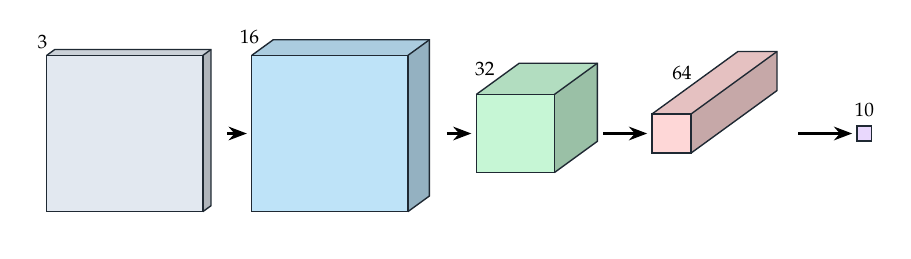
\begin{tikzpicture}[scale=0.62]
  \tensor{0}{0}{3.2}{3.2}{0.3}{cIn}{}{}{$3$}
  \tensor{4.2}{0}{3.2}{3.2}{0.8}{c16}{}{}{$16$}
  \tensor{8.8}{0.8}{1.6}{1.6}{1.6}{c32}{}{}{$32$}
  \tensor{12.4}{1.2}{0.8}{0.8}{3.2}{c64}{}{}{$64$}
  \matr{16.6}{1.45}{0.3}{0.3}{cG}{}{}{$10$}
  \foreach \a/\b in {3.7/4.1,8.2/8.7,11.4/12.3,15.4/16.5} \draw[-{Stealth},thick] (\a,1.6) -- (\b,1.6);
\end{tikzpicture}
\vspace{1.2cm}

{\large Lasfer Mohammed Djawed\par}
\vspace{0.2cm}
{\normalsize \href{https://github.com/fyl3x/resnet-cifar10}{\texttt{github.com/fyl3x/resnet-cifar10}}\par}
\vspace{0.2cm}
{\normalsize October 2026\par}
\vfill
\begin{minipage}{0.86\linewidth}\small
This document explains every step of the project: raw bytes, augmentation, normalisation, batching, every convolution, normalisation and shortcut, the logits and the loss, back-propagation through each operation, the optimiser, the schedule, evaluation and serving. It gives the shape of every tensor and the formula behind every number. The repository code is the source of truth: each claim about ``what the code does'' was checked against \texttt{cifar\_resnet/}, \texttt{scripts/} and \texttt{service/}, and the numerical examples were produced by running the trained checkpoint \texttt{model/resnet20.pt} on \texttt{samples/test0.png}. Reference: K.~He, X.~Zhang, S.~Ren, J.~Sun, \emph{Deep Residual Learning for Image Recognition}, CVPR 2016, \href{https://arxiv.org/abs/1512.03385}{arXiv:1512.03385}.
\end{minipage}
\vspace{0.8cm}
\end{titlepage}

\tableofcontents
\newpage
\section{The whole project on one page}
\label{sec:overview}

\subsection{What the project is}

The repository \href{https://github.com/fyl3x/resnet-cifar10}{\texttt{fyl3x/resnet-cifar10}} reproduces the CIFAR-10 ResNet of He et al.\ (2015), \emph{Deep Residual Learning for Image Recognition}, Section~4.2. The network is the $6n+2$ family with $n=3$ (ResNet-20) as the headline model and $n=9$ (ResNet-56) for the depth ablation. Everything is written in plain PyTorch: the blocks, the He initialisation, the augmentation, the iteration-based learning-rate schedule, the training loop and the metrics. The final model reaches \textbf{8.42\% test error} (paper: 8.75\%, both single runs) and is served by a FastAPI app inside a CPU Docker image.

\subsection{Pipeline at a glance}

\begin{center}
\resizebox{\linewidth}{!}{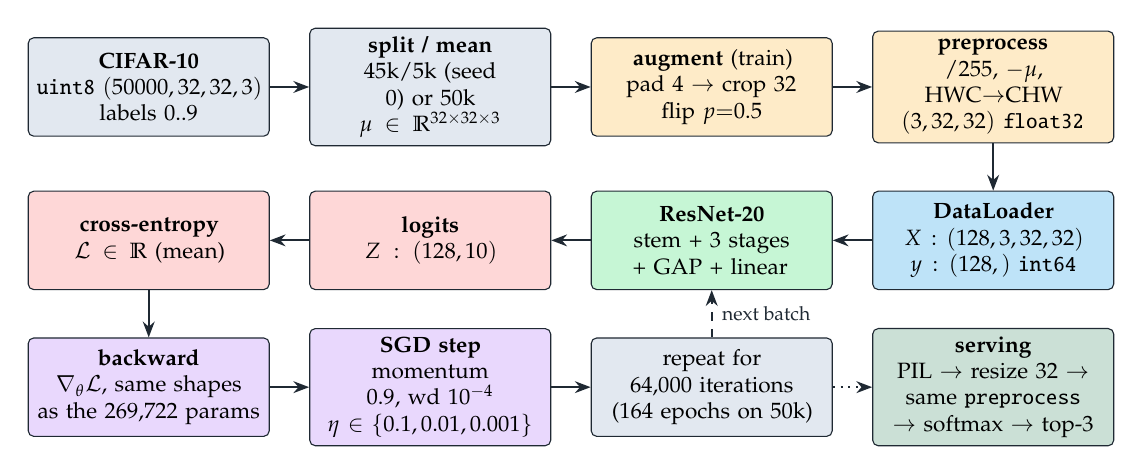
\begin{tikzpicture}[
  node distance=0.6cm and 0.5cm,
  box/.style={draw=ink,rounded corners=2pt,fill=#1,align=center,font=\footnotesize,minimum height=1.25cm,text width=2.85cm,inner sep=3pt},
  box/.default=cIn,
  ar/.style={-{Stealth[length=2mm]},thick,ink}]
  \node[box=cIn] (raw) {\textbf{CIFAR-10}\\ \code{uint8} $(50000,32,32,3)$\\labels $0..9$};
  \node[box=cIn,right=of raw] (split) {\textbf{split / mean}\\45k/5k (seed 0) or 50k\\$\mu\in\R^{32\times32\times3}$};
  \node[box=cK,right=of split] (aug) {\textbf{augment} (train)\\pad 4 $\to$ crop 32\\flip $p{=}0.5$};
  \node[box=cK,right=of aug] (pre) {\textbf{preprocess}\\$/255$, $-\mu$, HWC$\to$CHW\\$(3,32,32)$ \code{float32}};
  \node[box=c16,below=of pre] (batch) {\textbf{DataLoader}\\$X:(128,3,32,32)$\\$y:(128,)$ \code{int64}};
  \node[box=c32,left=of batch] (model) {\textbf{ResNet-20}\\stem + 3 stages\\+ GAP + linear};
  \node[box=c64,left=of model] (logits) {\textbf{logits}\\$Z:(128,10)$};
  \node[box=c64,left=of logits] (loss) {\textbf{cross-entropy}\\$\mathcal L\in\R$ (mean)};
  \node[box=cG,below=of loss] (back) {\textbf{backward}\\$\nabla_\theta\mathcal L$, same shapes\\as the 269{,}722 params};
  \node[box=cG,right=of back] (sgd) {\textbf{SGD step}\\momentum 0.9, wd $10^{-4}$\\$\eta\in\{0.1,0.01,0.001\}$};
  \node[box=cIn,right=of sgd] (loop) {repeat for 64{,}000 iterations\\(164 epochs on 50k)};
  \node[box=repo!25,right=of loop] (serve) {\textbf{serving}\\PIL $\to$ resize 32 $\to$ same \code{preprocess} $\to$ softmax $\to$ top-3};
  \draw[ar] (raw) -- (split); \draw[ar] (split) -- (aug); \draw[ar] (aug) -- (pre);
  \draw[ar] (pre) -- (batch); \draw[ar] (batch) -- (model); \draw[ar] (model) -- (logits); \draw[ar] (logits) -- (loss);
  \draw[ar] (loss) -- (back); \draw[ar] (back) -- (sgd); \draw[ar] (sgd) -- (loop);
  \draw[ar,dashed] (loop.north) -- (loop.north |- model.south) node[midway,right,font=\scriptsize]{next batch};
  \draw[ar,dotted] (loop) -- (serve);
\end{tikzpicture}}
\end{center}

\subsection{Code map}

\begin{center}
\small
\begin{tabularx}{\linewidth}{@{}>{\raggedright\arraybackslash}p{5.4cm}>{\raggedright\arraybackslash}X l@{}}
\toprule
File & What it contains & Explained in\\
\midrule
\file{cifar\_resnet/data.py} & \code{split\_indices}, \code{compute\_pixel\_mean}, \code{augment}, \code{preprocess}, \code{CIFARDataset} & \cref{sec:data}\\
\file{cifar\_resnet/model.py} & \code{BasicBlock} (residual or plain), \code{ResNetCIFAR} ($6n{+}2$, He init) & \cref{sec:block,sec:arch}\\
\file{cifar\_resnet/train.py} & \code{train\_step}, \code{train\_one\_epoch}, \code{evaluate}, \code{lr\_at}, \code{set\_lr}, checkpoints & \cref{sec:optim}\\
\file{cifar\_resnet/evaluate.py} & \code{predict} (softmax probs), confusion matrix, precision/recall/F1, ECE & \cref{sec:eval}\\
\file{scripts/train\_resnet.py} & CLI: \code{--n --plain --seed --full --name --max-iters}; builds data, model, SGD, logs CSV & \cref{sec:optim}\\
\file{scripts/eval\_test.py}, \file{scripts/make\_report.py}, \file{scripts/make\_ablation.py} & test-set evaluation, figures, ablation table & \cref{sec:eval}\\
\file{service/app.py} & FastAPI: \code{GET /health}, \code{POST /predict} & \cref{sec:serving}\\
\file{scripts/check\_*.py}, \file{overfit\_batch.py} & the development checks run at each stage & throughout\\
\bottomrule
\end{tabularx}
\end{center}

\subsection{The configuration that every number in this document assumes}
\label{sec:config}

\begin{center}
\small\setlength{\tabcolsep}{4pt}
\begin{tabular}{@{}lll@{}}
\toprule
Quantity & Value in this repo & Where it is set\\
\midrule
Depth parameter $n$ & 3 (ResNet-20); 9 for ResNet-56 & \code{--n}, \code{ResNetCIFAR(n)}\\
Stage widths & $(16, 32, 64)$ & \code{widths=(16,32,64)}\\
Residual or plain & residual; \code{--plain} removes the shortcut & \code{BasicBlock(residual=...)}\\
Shortcut & option A: stride-2 subsample + zero channel padding & \code{BasicBlock.forward}\\
Classes & 10 & \code{num\_classes=10}\\
Batch size $N$ & 128 & \code{DataLoader(batch\_size=128)}\\
Optimiser & SGD, momentum $\mu=0.9$, weight decay $\lambda=10^{-4}$ & \file{train\_resnet.py}\\
Learning rate $\eta$ & 0.1 / 0.01 / 0.001, switching at iterations 32k / 48k & \code{lr\_at}\\
Iterations & 64{,}000 & \code{--max-iters}\\
Loss & \code{nn.CrossEntropyLoss()} (mean over batch) & \file{train\_resnet.py}\\
Initialisation & He normal, $\sigma=\sqrt{2/\text{fan\_in}}$, convs only & \code{\_init\_weights}\\
Final training set & all 50{,}000 images (\code{--full}) & \file{train\_resnet.py}\\
Development split & 45{,}000 / 5{,}000, split seed fixed to 0 & \code{split\_indices(50000,5000,0)}\\
Parameters & 269{,}722 (ResNet-20), 853{,}018 (ResNet-56) & counted from the model\\
\bottomrule
\end{tabular}
\end{center}

\subsection{Notation}

\begin{center}
\small
\begin{tabular}{@{}ll@{\qquad}ll@{}}
\toprule
$N$ & batch size (128) & $\mathcal W$ & 4-D conv weight $(C_\text{out},C_\text{in},K,K)$\\
$C,H,W$ & channels, height, width & $W$ (linear) & weight matrix $(10,64)$\\
$K,S,P$ & kernel size, stride, padding & $\gamma,\beta$ & BN scale and shift, shape $(C,)$\\
$x$, $X$ & one input / a batch & $\mu_c,\sigma_c^2$ & BN batch mean and variance of channel $c$\\
$\mathcal F(x)$ & residual branch of a block & $z$, $Z$ & logits of one image / a batch\\
$s$ & softmax probabilities & $\mathcal L$ & mean cross-entropy over the batch\\
$G_T$ & $\partial\mathcal L/\partial T$, \emph{same shape as $T$} & $\eta,\mu,\lambda$ & learning rate, momentum, weight decay\\
\bottomrule
\end{tabular}
\end{center}

Shapes are written in PyTorch order, e.g.\ \shp{128,16,32,32}. In drawings, a box of width $W$ and height $H$ with depth going into the page is one image's feature tensor, and the depth is its channel count. Box colours follow the stage: \colorbox{cIn}{input}, \colorbox{c16}{16 channels}, \colorbox{c32}{32 channels}, \colorbox{c64}{64 channels}, \colorbox{cK}{weights}, \colorbox{cG}{outputs/gradients}.

Each section separates the \textcolor{idea}{\textbf{general idea}} (what the mathematics says, independent of this code), \textcolor{repo}{\textbf{in this repository}} (what the code actually does, with sizes), \textcolor{warn}{\textbf{details and deviations}} (where the code differs from a textbook or a reader could be surprised), and \textcolor{shapec}{\textbf{shape checks}}.

\section{Data: from bytes on disk to a batch tensor}
\label{sec:data}

\subsection{Raw CIFAR-10 as torchvision hands it over}

\begin{repo}[\texttt{torchvision.datasets.CIFAR10(root="data", train=..., download=True)}]
The dataset object exposes two plain attributes, and the repo uses them directly. It never goes through torchvision's transforms or its \code{\_\_getitem\_\_}:
\begin{itemize}[nosep]
  \item \code{data.data}: a NumPy array of shape \shp{50000,32,32,3} for \code{train=True} or \shp{10000,32,32,3} for \code{train=False}, \code{dtype=uint8}, values $0..255$, channel order RGB, layout \emph{HWC}.
  \item \code{data.targets}: a Python \code{list} of 50{,}000 (or 10{,}000) integers in $0..9$.
\end{itemize}
Class indices: 0~airplane, 1~automobile, 2~bird, 3~cat, 4~deer, 5~dog, 6~frog, 7~horse, 8~ship, 9~truck. Training has 5{,}000 images per class and test has 1{,}000 per class.
\end{repo}

\begin{center}
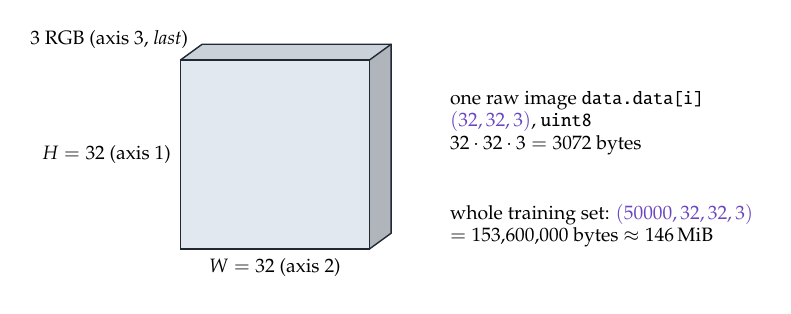
\begin{tikzpicture}
  \tensor{0}{0}{2.4}{2.4}{0.5}{cIn}{$W=32$ (axis 2)}{$H=32$ (axis 1)}{$3$ RGB (axis 3, \emph{last})}
  \node[font=\scriptsize,align=left,right] at (3.3,1.6) {one raw image \code{data.data[i]}\\ \shp{32,32,3}, \code{uint8}\\ $32\cdot32\cdot3 = 3072$ bytes};
  \node[font=\scriptsize,align=left,right] at (3.3,0.3) {whole training set: \shp{50000,32,32,3}\\ $=153{,}600{,}000$ bytes $\approx 146$\,MiB};
\end{tikzpicture}
\end{center}

\subsection{Train / validation split}

\begin{lstlisting}[firstnumber=5]
def split_indices(n,n_val,seed):
    g = torch.Generator()
    g.manual_seed(seed)
    result = torch.randperm(n=n,generator=g)
    validation_idx = result[:n_val]
    training_idx = result[n_val:]
    return training_idx,validation_idx
\end{lstlisting}

\begin{idea}
Draw one random permutation of $\{0,\dots,n-1\}$ and cut it: the first $n_\text{val}$ indices are validation and the rest are training. The two sets are disjoint and together cover everything. This is checked in \file{scripts/check\_split.py}: 45{,}000 + 5{,}000, zero overlap, same seed $\Rightarrow$ same split.
\end{idea}

\begin{repo}[two regimes]
\begin{itemize}[nosep]
  \item \textbf{Development} (default, used for all four ablation runs): \code{split\_indices(50000, 5000, 0)} gives 45{,}000 training and 5{,}000 validation indices, both \code{int64} tensors.
  \item \textbf{Final} (\code{--full}): \code{train\_idx = torch.arange(50000)}, with no validation set. The test set (10{,}000) is used only once, in \file{eval\_test.py}.
\end{itemize}
\end{repo}

\begin{warn}[the split seed is hard-coded]
\file{train\_resnet.py} calls \code{split\_indices(50000,5000,0)} with a literal \code{0}, not \code{args.seed}. Changing \code{--seed} changes the initialisation, the shuffling and the augmentation, but \emph{not} which 5{,}000 images are held out. This is deliberate: the 45k mean file \code{pixel\_mean\_45k\_seed0.npy} is only valid for that split.
\end{warn}

\subsection{Per-pixel mean}
\label{sec:mean}

\begin{lstlisting}[firstnumber=13]
def compute_pixel_mean(images,train_idx):
    training_images = images[train_idx.numpy()]
    floated_images = training_images.astype(np.float32)
    avg = floated_images.mean(axis=0)
    avg /= 255
    return avg
\end{lstlisting}

\begin{idea}[mean over images, not over pixels]
With $\mathcal T$ the set of training indices,
\[
  \mu[h,w,c] \;=\; \frac{1}{255\,|\mathcal T|}\sum_{i\in\mathcal T} x_i[h,w,c], \qquad \mu\in\R^{32\times32\times3}.
\]
This is a \emph{per-pixel, per-channel} mean: 3{,}072 separate numbers, an ``average image''. Contrast it with the more common \emph{per-channel} mean (3 numbers, the average over images \emph{and} positions). The paper says ``the per-pixel mean subtracted'', and that is what this repo implements.
\end{idea}

\begin{center}
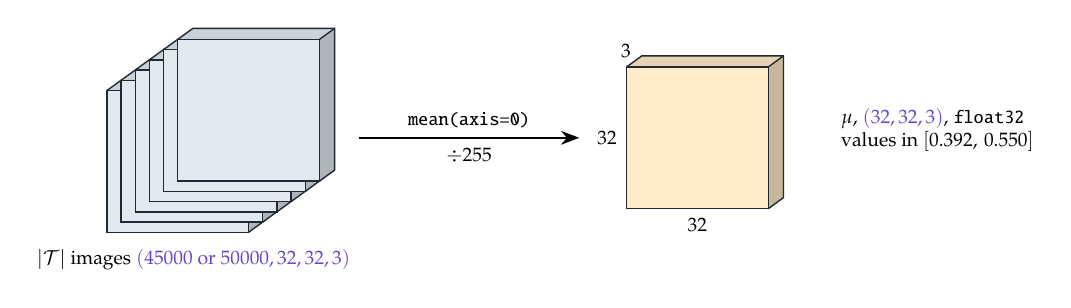
\begin{tikzpicture}
  \foreach \k in {0,...,5} {\tensor{0.18*\k}{0.13*\k}{1.8}{1.8}{0.35}{cIn}{}{}{}}
  \node[font=\scriptsize] at (1.1,-0.35) {$|\mathcal T|$ images \shp{45000\text{ or }50000,32,32,3}};
  \draw[-{Stealth},thick] (3.2,1.2) -- (6.0,1.2) node[midway,above,font=\scriptsize]{\code{mean(axis=0)}} node[midway,below,font=\scriptsize]{$\div 255$};
  \tensor{6.6}{0.3}{1.8}{1.8}{0.35}{cK}{$32$}{$32$}{$3$}
  \node[font=\scriptsize,align=left,right] at (9.2,1.3) {$\mu$, \shp{32,32,3}, \code{float32}\\ values in $[0.392,\,0.550]$};
\end{tikzpicture}
\end{center}

\begin{repo}[the actual mean file \texttt{model/pixel\_mean\_50k.npy}]
Shape \shp{32,32,3}, \code{float32}, 12{,}416 bytes on disk (12{,}288 data + header). Averaged over positions, the three channels are $(0.4914,\;0.4822,\;0.4465)$, the familiar CIFAR-10 channel means. Individual entries range from $0.392$ to $0.550$; for example $\mu[0,0]=(0.513,0.534,0.520)$ at the top-left corner and $\mu[16,16]=(0.502,0.457,0.421)$ at the centre. The corner is greyer and the centre more reddish, which is where objects usually sit. Two files exist: \code{pixel\_mean\_45k\_seed0.npy} (development split) and \code{pixel\_mean\_50k.npy} (final model and service). The mean is always computed on the raw, \emph{un-augmented} training images.
\end{repo}

\begin{warn}[no division by a standard deviation]
\code{preprocess} subtracts the mean and does not divide by any standard deviation. The paper does not mention one either, and BN right after the stem rescales the activations anyway. Inputs therefore keep the raw $[0,1]$ spread, roughly $[-0.55,\,0.61]$ after centring.
\end{warn}

\subsection{Augmentation (training only)}
\label{sec:augment}

\begin{lstlisting}[firstnumber=20]
def augment(image,rng):
    padded_image = np.pad(image,pad_width=((4, 4), (4, 4), (0, 0)))
    top_offset = rng.integers(0,9)
    left_offset = rng.integers(0,9)
    cropped_image = padded_image[top_offset:top_offset+32, left_offset:left_offset+32, :]
    if rng.random() < 0.5 :
        cropped_image = np.ascontiguousarray(np.flip(cropped_image, axis=1))
    return cropped_image
\end{lstlisting}

\begin{center}
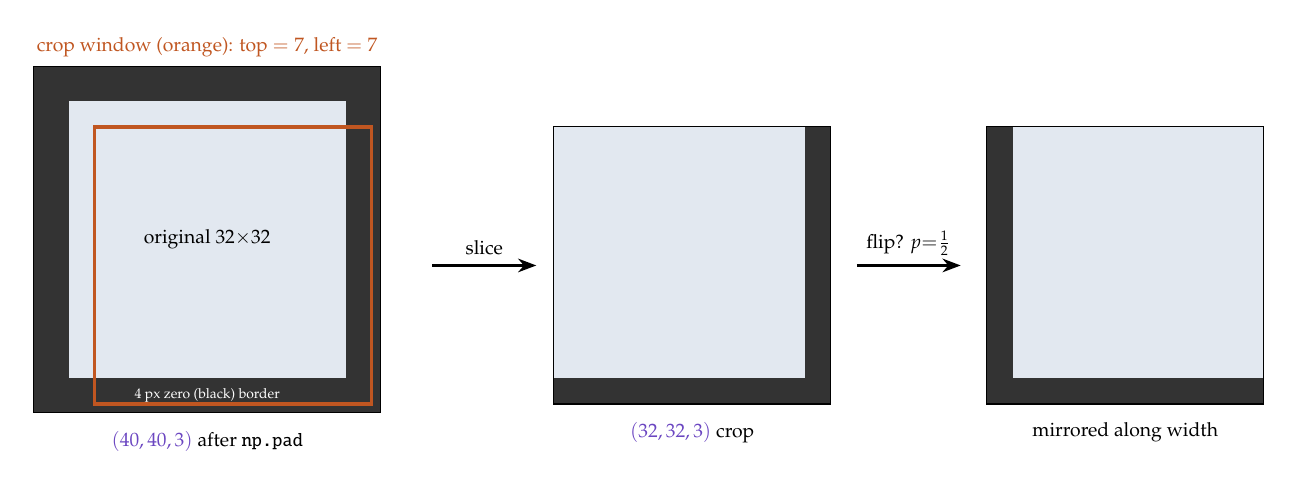
\begin{tikzpicture}[scale=0.11]
  % padded 40x40
  \fill[black!80] (0,0) rectangle (40,40);
  \fill[cIn] (4,4) rectangle (36,36);
  \draw (0,0) rectangle (40,40);
  \node[font=\tiny,white] at (20,2) {4 px zero (black) border};
  \node[font=\scriptsize] at (20,20) {original $32{\times}32$};
  \draw[warn,line width=1.2pt] (7,1) rectangle (39,33);
  \node[warn,font=\scriptsize,above] at (20,40) {crop window (orange): top $=7$, left $=7$};
  \node[below,font=\scriptsize] at (20,-1) {\shp{40,40,3} after \code{np.pad}};
  \draw[-{Stealth},thick] (46,17) -- (58,17) node[midway,above,font=\scriptsize]{slice};
  \fill[black!80] (60,1) rectangle (92,33);
  \fill[cIn] (60,4) rectangle (89,33);
  \draw (60,1) rectangle (92,33);
  \node[below,font=\scriptsize] at (76,0) {\shp{32,32,3} crop};
  \draw[-{Stealth},thick] (95,17) -- (107,17) node[midway,above,font=\scriptsize]{flip? $p{=}\frac12$};
  \fill[black!80] (110,1) rectangle (142,33);
  \fill[cIn] (113,4) rectangle (142,33);
  \draw (110,1) rectangle (142,33);
  \node[below,font=\scriptsize] at (126,0) {mirrored along width};
\end{tikzpicture}
\end{center}

\begin{idea}
Random translation by up to $\pm4$ pixels plus a random left--right mirror. The label stays the same, and the network sees a slightly different image every epoch. This is the standard ``pad 4, random crop 32, horizontal flip'' of the paper.
\end{idea}

\begin{repo}[exact behaviour]
\begin{itemize}[nosep]
  \item \code{np.pad} with no mode means constant \textbf{0}, applied to the \code{uint8} image, so the border is pure black \emph{before} normalisation.
  \item \code{rng.integers(0,9)} draws from $\{0,1,\dots,8\}$ (upper bound exclusive): 9 vertical $\times$ 9 horizontal offsets $=81$ crop positions, and offset 4 is the un-shifted image. With the flip, that gives up to $162$ distinct views of each image.
  \item \code{np.flip(axis=1)} reverses the \emph{width} axis of an HWC array, which is a horizontal mirror. \code{np.flip} returns a negative-stride view, so \code{np.ascontiguousarray} copies it into normal memory.
  \item Three random draws per image, in order: top offset, left offset, flip coin.
  \item \code{CIFARDataset} owns \emph{one} \code{np.random.default\_rng(seed)} created in \code{\_\_init\_\_}, used only when \code{train=True}. Its stream is consumed in the order the sampler requests images, so the whole augmentation sequence is reproducible given the seed.
\end{itemize}
\end{repo}

\begin{warn}[two subtle consequences]
\textbf{(1) Padding is not zero after preprocessing.} Pixels in the black border become $0/255-\mu[h,w,c]\approx(-0.49,-0.48,-0.45)$, not 0. The network sees ``black'', which is a legitimate image colour. It is \emph{not} the same as the zero padding inside the convolutions. Common pipelines that pad a PIL image before normalising behave the same way.

\textbf{(2) The RNG would be duplicated by worker processes.} With \code{DataLoader(num\_workers>0)}, each worker gets a copy of the same \code{rng} state, so different workers would produce identical augmentation sequences. The repo uses the default \code{num\_workers=0} (single process), so this does not happen. It is something to remember before ``speeding up'' the loader.
\end{warn}

\subsection{Preprocessing: the function shared by training and serving}
\label{sec:preprocess}

\begin{lstlisting}[firstnumber=29]
def preprocess(image,mean):
    image = image.astype(np.float32)
    image = image / 255
    image = image - mean
    tensored_image = torch.tensor(image)
    tensored_image = tensored_image.permute(2,0,1).contiguous()
    return tensored_image
\end{lstlisting}

\begin{center}
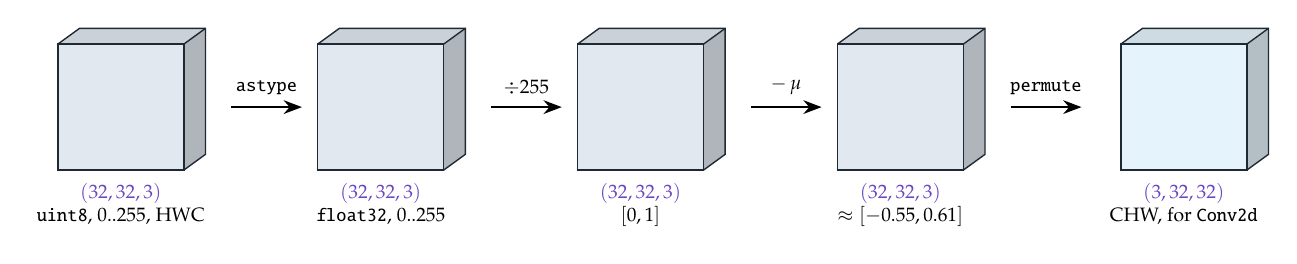
\begin{tikzpicture}
  \foreach \k/\xx/\lab/\top in {0/0/{\code{uint8}, $0..255$, HWC}/{raw},1/3.3/{\code{float32}, $0..255$}/{\code{astype}},2/6.6/{$[0,1]$}/{$\div 255$},3/9.9/{$\approx[-0.55,0.61]$}/{$-\,\mu$}} {
    \tensor{\xx}{0}{1.6}{1.6}{0.5}{cIn}{}{}{}
    \node[font=\scriptsize,below,align=center] at (\xx+0.8,-0.05) {\shp{32,32,3}\\\lab};
  }
  \foreach \xx/\op in {2.2/{\code{astype}},5.5/{$\div255$},8.8/{$-\,\mu$},12.1/{\code{permute}}}
    \draw[-{Stealth},thick] (\xx,0.8) -- (\xx+0.9,0.8) node[midway,above=3pt,font=\scriptsize,fill=white,inner sep=1pt]{\op};
  \tensor{13.5}{0}{1.6}{1.6}{0.5}{c16!40}{}{}{}
  \node[font=\scriptsize,below,align=center] at (14.3,-0.05) {\shp{3,32,32}\\CHW, for \code{Conv2d}};
\end{tikzpicture}
\end{center}

\begin{idea}[why the permute]
NumPy, PIL and torchvision store images channel-last (HWC). \code{nn.Conv2d} expects channel-first (CHW, and NCHW for a batch). \code{permute(2,0,1)} reorders the axes: new axis 0 = old axis 2 (channels), new 1 = old 0 (rows), new 2 = old 1 (columns). Mathematically, $X_\text{out}[c,h,w] = X_\text{in}[h,w,c]$. \code{permute} only changes strides, and \code{.contiguous()} materialises a copy laid out in the new order.
\end{idea}

\begin{repo}[broadcasting in $\text{image}-\mu$]
Both operands are \shp{32,32,3}, so the subtraction is element-wise with no broadcasting: each pixel subtracts \emph{its own} mean. Worked example from \file{samples/test0.png} (a cat): raw top-left pixel $(158,112,49)$, so $(0.6196,0.4392,0.1922)-(0.5126,0.5336,0.5198)=(0.1070,-0.0943,-0.3277)$, which is exactly \code{x[0,:,0,0]} in the model input. Over the whole image the values lie in $[-0.438,\,0.591]$ with mean $-0.048$.
\end{repo}

\subsection{Dataset and batching}

\begin{lstlisting}[firstnumber=37]
class CIFARDataset(torch.utils.data.Dataset):
    ...
    def __getitem__(self, i):
        idx = int(self.indices[i])
        image, label = self.images[idx], self.labels[idx]
        if self.train:
            image = augment(image=image,rng=self.rng)
        return preprocess(image, self.mean), label
\end{lstlisting}

\begin{idea}[indirection through \texttt{indices}]
The dataset never copies the images. It keeps the full array plus an index list, and position $i$ in the dataset maps to raw image \code{indices[i]}. The same object therefore serves the 45k split, the 5k split, the full 50k and the 10k test set.
\end{idea}

\begin{center}
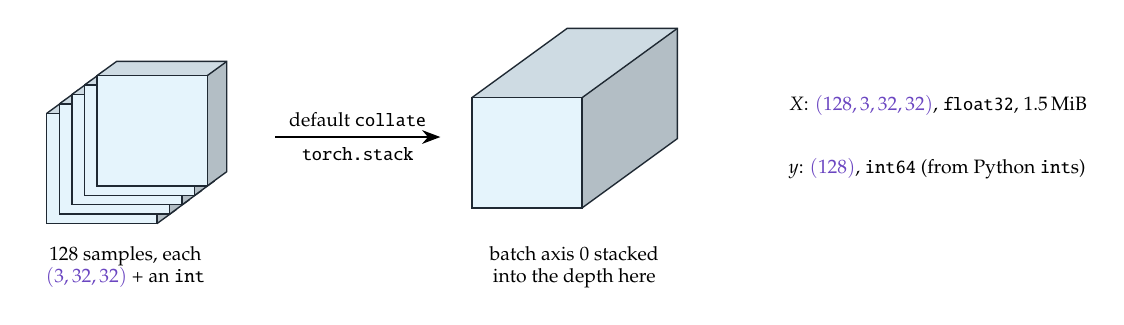
\begin{tikzpicture}
  \foreach \k in {0,...,4} {\tensor{0.16*\k}{0.12*\k}{1.4}{1.4}{0.45}{c16!40}{}{}{}}
  \node[font=\scriptsize,align=center] at (1.0,-0.55) {128 samples, each\\ \shp{3,32,32} + an \code{int}};
  \draw[-{Stealth},thick] (2.9,1.1) -- (5.0,1.1) node[midway,above,font=\scriptsize]{default \code{collate}} node[midway,below,font=\scriptsize]{\code{torch.stack}};
  \tensor{5.4}{0.2}{1.4}{1.4}{2.2}{c16!40}{}{}{}
  \node[font=\scriptsize,align=center] at (6.7,-0.55) {batch axis 0 stacked\\ into the depth here};
  \node[font=\scriptsize,align=left,right] at (9.3,1.5) {$X$: \shp{128,3,32,32}, \code{float32}, 1.5\,MiB};
  \node[font=\scriptsize,align=left,right] at (9.3,0.7) {$y$: \shp{128}, \code{int64} (from Python \code{int}s)};
\end{tikzpicture}
\end{center}

\begin{repo}[loaders and the number of batches]
\begin{itemize}[nosep]
  \item Training: \code{DataLoader(batch\_size=128, shuffle=True, generator=g)} with \code{g} seeded by \code{--seed}. A new random order is drawn from \code{g} every epoch. \code{drop\_last} is \code{False}, so the remainder forms a short final batch.
  \item Validation and test: \code{shuffle=False}, \code{train=False}, so there is no augmentation.
\end{itemize}
\begin{center}
\begin{tabular}{@{}lrrrr@{}}
\toprule
set & images & full batches & last batch & batches per pass\\
\midrule
final training (50k) & 50{,}000 & 390 & 80 & \textbf{391}\\
development training (45k) & 45{,}000 & 351 & 72 & \textbf{352}\\
validation & 5{,}000 & 39 & 8 & 40\\
test & 10{,}000 & 78 & 16 & 79\\
\bottomrule
\end{tabular}
\end{center}
These numbers fix the epoch arithmetic of \cref{sec:schedule}: one epoch on 50k is 391 \emph{iterations}, and the schedule counts iterations, not epochs.
\end{repo}

\section{The mathematical toolkit, one operation at a time}
\label{sec:toolkit}

Every layer in ResNet-20 is one of six operations: matrix multiplication (inside the linear layer), 2-D convolution, batch normalisation, ReLU, global average pooling, and the softmax/cross-entropy pair at the end. This section treats each one on its own, first in general, then with the exact sizes this repository uses. Sections~\ref{sec:block} and~\ref{sec:arch} then just compose them.

%-------------------------------------------------------------------
\subsection{Matrix multiplication and how shapes align}
\label{sec:matmul}

\begin{idea}[the inner dimensions must match and disappear]
For $A\in\R^{m\times k}$ and $B\in\R^{k\times n}$, the product $C=AB\in\R^{m\times n}$ is
\[
  C_{ij} \;=\; \sum_{t=1}^{k} A_{it}\,B_{tj}, \qquad i=1..m,\; j=1..n .
\]
Entry $C_{ij}$ is the dot product of \emph{row $i$ of $A$} with \emph{column $j$ of $B$}, so both must have length $k$. The shared (inner) dimension $k$ is summed away; the outer dimensions $m$ and $n$ survive:
\[
  \underbrace{(m\times \cancel{k})}_{A}\;\cdot\;\underbrace{(\cancel{k}\times n)}_{B}\;=\;\underbrace{(m\times n)}_{C},
  \qquad \text{cost} = m\,k\,n \text{ multiply--adds.}
\]
\end{idea}

The picture below is the one to keep in your head: put $B$ above $C$ and $A$ to its left. Then every cell of $C$ sits at the crossing of one row of $A$ and one column of $B$.

\begin{center}
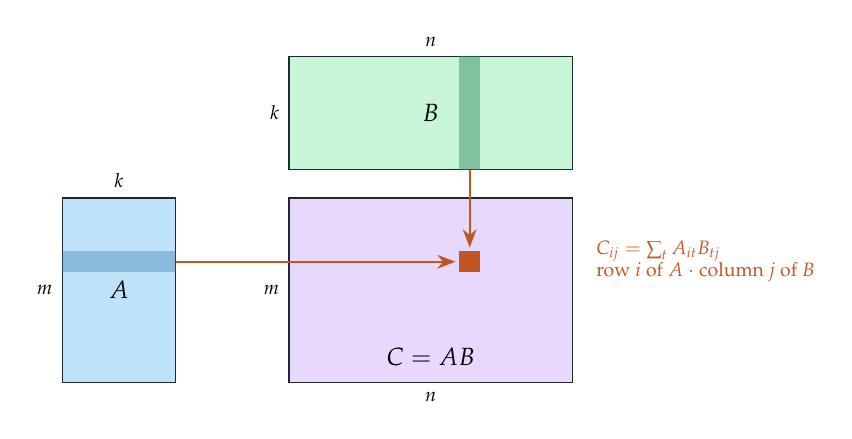
\begin{tikzpicture}[scale=0.9]
  % B on top
  \matr{3.2}{3.0}{4.0}{1.6}{c32}{$B$}{$k$}{$n$}
  % A left
  \matr{0}{0}{1.6}{2.6}{c16}{$A$}{$m$}{$k$}
  % C
  \matr{3.2}{0}{4.0}{2.6}{cG}{}{$m$}{}
  \node[font=\small] at (5.2,0.35) {$C=AB$};
  \node[below,font=\scriptsize] at (5.2,0) {$n$};
  % highlight row and column
  \fill[idea,opacity=0.35] (0,1.55) rectangle (1.6,1.85);
  \fill[repo,opacity=0.45] (5.6,3.0) rectangle (5.9,4.6);
  \fill[warn] (5.6,1.55) rectangle (5.9,1.85);
  \draw[-{Stealth},warn,thick] (1.6,1.7) -- (5.55,1.7);
  \draw[-{Stealth},warn,thick] (5.75,3.0) -- (5.75,1.9);
  \node[warn,font=\scriptsize,align=left,right] at (7.4,1.7) {$C_{ij}=\sum_t A_{it}B_{tj}$\\row $i$ of $A$ $\cdot$ column $j$ of $B$};
\end{tikzpicture}
\end{center}

\begin{repo}[where matrix multiplication appears]
Explicitly, only once: the final \code{nn.Linear(64, 10)}. Implicitly, every convolution is a matrix multiplication after the \emph{im2col} rearrangement (\cref{sec:im2col}). Batch normalisation, ReLU and pooling are not matrix multiplications.
\end{repo}

%-------------------------------------------------------------------
\subsection{The fully connected (linear) layer}
\label{sec:linear}

\begin{idea}[affine map, PyTorch convention]
PyTorch stores the weight of \code{nn.Linear(in, out)} as $W\in\R^{\text{out}\times\text{in}}$ and computes, for a batch $X\in\R^{N\times\text{in}}$ (one example per row),
\[
  Z \;=\; X\,W\T + \mathbf{1}_N\, b\T, \qquad Z\in\R^{N\times\text{out}}, \quad b\in\R^{\text{out}} .
\]
Each row $z_n = W x_n + b$ is the textbook ``$Wx+b$''; stacking examples as rows is what turns it into $XW\T$. The bias row is \emph{broadcast}: the same $b$ is added to every one of the $N$ rows.
\end{idea}

\begin{center}
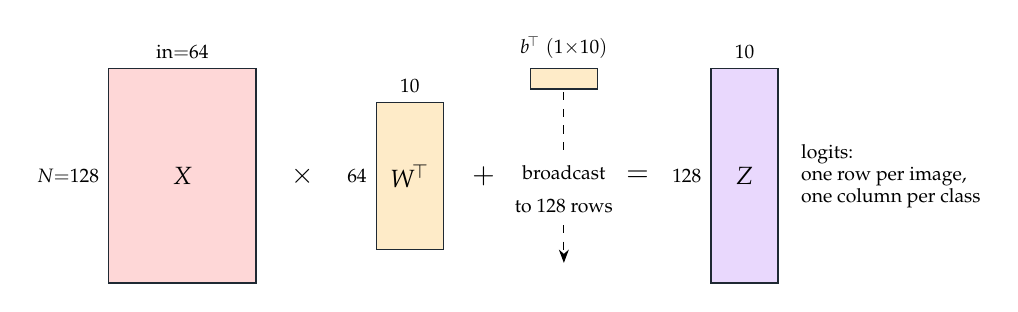
\begin{tikzpicture}[scale=0.85]
  \matr{0}{0}{2.2}{3.2}{c64}{$X$}{$N{=}128$}{$\text{in}{=}64$}
  \node at (2.9,1.6) {$\times$};
  \matr{4.0}{0.5}{1.0}{2.2}{cK}{$W\T$}{$64$}{$10$}
  \node at (5.6,1.6) {$+$};
  \matr{6.3}{2.9}{1.0}{0.3}{cK}{}{}{$b\T\;(1{\times}10)$}
  \draw[-{Stealth},dashed] (6.8,2.85) -- (6.8,0.3);
  \node[font=\scriptsize,align=center] at (6.8,1.4) {\colorbox{white}{broadcast}\\\colorbox{white}{to 128 rows}};
  \node at (7.9,1.6) {$=$};
  \matr{9.0}{0}{1.0}{3.2}{cG}{$Z$}{$128$}{$10$}
  \node[right,font=\scriptsize,align=left] at (10.2,1.6) {logits:\\ one row per image,\\ one column per class};
\end{tikzpicture}
\end{center}

\begin{repo}[\texttt{self.linear = nn.Linear(64, 10)}]
$W\in\R^{10\times 64}$ (640 numbers) and $b\in\R^{10}$ (10 numbers): 650 parameters, the only layer with a bias in the whole network. Its input is the 64-dimensional pooled feature vector of each image, its output the 10 logits. This is the only fully connected (``feed-forward'') layer in the model: there is no hidden MLP head, no dropout.
\end{repo}

%-------------------------------------------------------------------
\subsection{Tensors and the meaning of every axis}
\label{sec:axes}

\begin{idea}[NCHW]
A batch of images is a 4-D tensor $X\in\R^{N\times C\times H\times W}$. I draw one image ($N$ fixed) as a box: width $W$ to the right, height $H$ upward, and \emph{depth} $C$ going into the page. Each depth slice $X[n,c,:,:]$ is one $H\times W$ \emph{feature map}; each depth fibre $X[n,:,h,w]$ is the $C$-vector describing location $(h,w)$.
\end{idea}

\begin{center}
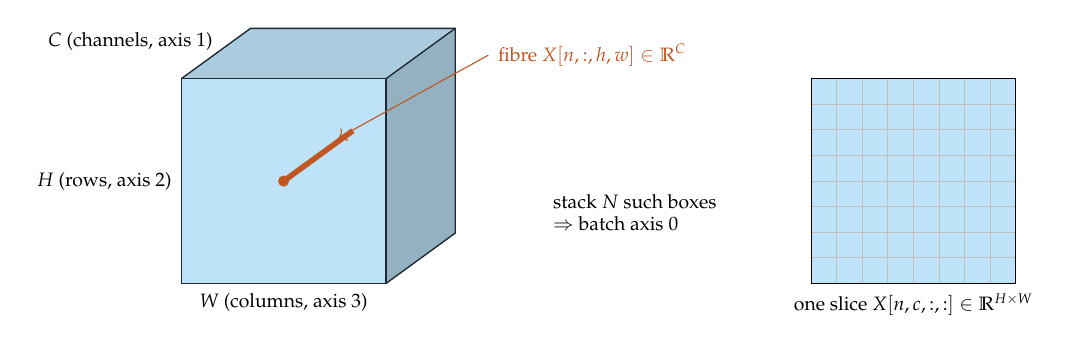
\begin{tikzpicture}
  \tensor{0}{0}{2.6}{2.6}{1.6}{c16}{$W$ (columns, axis 3)}{$H$ (rows, axis 2)}{$C$ (channels, axis 1)}
  % one fibre
  \draw[warn,line width=2pt] (1.3,1.3) -- ++(0.55*1.6,0.40*1.6);
  \fill[warn] (1.3,1.3) circle (2pt);
  \node[warn,font=\scriptsize,right] at (3.9,2.9) {fibre $X[n,:,h,w]\in\R^{C}$};
  \draw[warn,->] (3.9,2.9) -- (2.0,1.85);
  \node[font=\scriptsize,align=left,right] at (4.6,0.9) {stack $N$ such boxes\\$\Rightarrow$ batch axis 0};
  % slice
  \begin{scope}[shift={(8,0)}]
    \fill[c16] (0,0) rectangle (2.6,2.6); \draw (0,0) rectangle (2.6,2.6);
    \foreach \i in {0.325,0.65,...,2.6} {\draw[black!25] (\i,0) -- (\i,2.6); \draw[black!25] (0,\i) -- (2.6,\i);}
    \draw (0,0) rectangle (2.6,2.6);
    \node[below,font=\scriptsize] at (1.3,0) {one slice $X[n,c,:,:]\in\R^{H\times W}$};
  \end{scope}
\end{tikzpicture}
\end{center}

\begin{repo}[axis meaning at each point of the pipeline]
\begin{tabularx}{\linewidth}{@{}>{\raggedright\arraybackslash}p{3.3cm}>{\raggedright\arraybackslash}p{4.9cm}l>{\raggedright\arraybackslash}X@{}}
\toprule
Where & Layout & dtype & Meaning \\
\midrule
\code{data.data} (torchvision) & $(50000,32,32,3)$ & \code{uint8} & images, \emph{HWC} order, values $0..255$ \\
inside \code{augment} & $(32,32,3)\!\to\!(40,40,3)\!\to\!(32,32,3)$ & \code{uint8} & one image, still HWC \\
output of \code{preprocess} & $(3,32,32)$ & \code{float32} & CHW, mean-subtracted \\
a training batch & $(128,3,32,32)$ & \code{float32} & NCHW, what the model eats \\
labels batch & $(128,)$ & \code{int64} & class index $0..9$ per image \\
logits & $(128,10)$ & \code{float32} & one score per (image, class) \\
\bottomrule
\end{tabularx}
\end{repo}

%-------------------------------------------------------------------
\subsection{2-D convolution}
\label{sec:conv}

\begin{idea}[what \texttt{nn.Conv2d} computes]
A convolution layer with $C_\text{in}$ input channels, $C_\text{out}$ output channels, kernel size $K$, stride $S$ and zero padding $P$ has a weight tensor
\[
  \mathcal W \in \R^{C_\text{out}\times C_\text{in}\times K\times K}.
\]
Pad the input with $P$ zeros on every side, $\tilde X[n,c,a,b] = X[n,c,a-P,b-P]$ (zero outside the image). Then, with no bias,
\[
  \boxed{\;Y[n,o,i,j] \;=\; \sum_{c=0}^{C_\text{in}-1}\;\sum_{u=0}^{K-1}\;\sum_{v=0}^{K-1}
  \mathcal W[o,c,u,v]\;\tilde X[n,\,c,\,S i+u,\,S j+v]\;}
\]
Strictly this is a cross-correlation (the kernel is not flipped). Deep-learning libraries call it convolution anyway. Since the weights are learned, the difference does not matter.

Three facts to keep:
\begin{enumerate}[nosep]
  \item \textbf{Each filter $\mathcal W[o]$ is a $C_\text{in}\times K\times K$ block}, as deep as the input. It sums over \emph{all} input channels and produces \emph{one} 2-D map.
  \item \textbf{The number of filters is the output depth.} $C_\text{out}$ filters give $C_\text{out}$ maps, stacked along axis~1. This is how depth ``is added''.
  \item \textbf{Spatial size} follows from the window positions that fit:
  \[
    H_\text{out} = \left\lfloor \frac{H_\text{in} + 2P - K}{S} \right\rfloor + 1, \qquad W_\text{out}\text{ likewise.}
  \]
\end{enumerate}
\end{idea}

\begin{center}
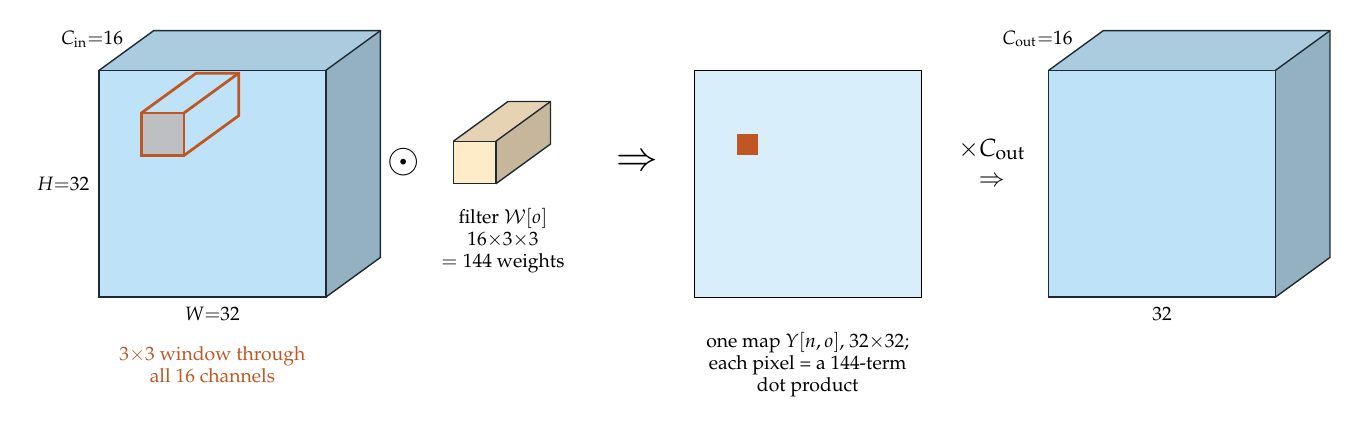
\begin{tikzpicture}[scale=0.9]
  \tensor{0}{0}{3.2}{3.2}{1.4}{c16}{$W{=}32$}{$H{=}32$}{$C_\text{in}{=}16$}
  \draw[warn,line width=1pt,fill=warn,fill opacity=0.25] (0.6,2.0) rectangle (1.2,2.6);
  \draw[warn,line width=1pt] (0.6,2.6) -- ++(0.77,0.56) -- ++(0.6,0) -- ++(0,-0.6) -- (1.2,2.0);
  \draw[warn,line width=1pt] (1.2,2.6) -- ++(0.77,0.56);
  \node[warn,font=\scriptsize,align=center] at (1.6,-0.95) {$3{\times}3$ window through\\all 16 channels};
  \tensor{5.0}{1.6}{0.6}{0.6}{1.4}{cK}{}{}{}
  \node[font=\scriptsize,align=center] at (5.7,0.8) {filter $\mathcal W[o]$\\$16{\times}3{\times}3$\\$=144$ weights};
  \node[font=\Large] at (4.3,1.9) {$\odot$};
  \node[font=\Large] at (7.6,1.9) {$\Rightarrow$};
  \begin{scope}[shift={(8.4,0)}]
    \fill[c16!60] (0,0) rectangle (3.2,3.2); \draw (0,0) rectangle (3.2,3.2);
    \fill[warn] (0.6,2.0) rectangle (0.9,2.3);
    \node[font=\scriptsize,align=center] at (1.6,-0.95) {one map $Y[n,o]$, $32{\times}32$;\\each pixel = a 144-term\\dot product};
  \end{scope}
  \node[font=\small,align=center] at (12.6,1.9) {$\times C_\text{out}$\\$\Rightarrow$};
  \tensor{13.4}{0}{3.2}{3.2}{1.4}{c16}{$32$}{}{$C_\text{out}{=}16$}
\end{tikzpicture}
\end{center}

\paragraph{Worked output-size examples (all convolutions in this repo use $K=3$, $P=1$).}
\begin{align*}
  S=1:&\quad H_\text{out}=\left\lfloor\tfrac{32+2-3}{1}\right\rfloor+1 = 31+1 = 32 &&\text{(``same'' padding: size preserved)}\\
  S=1:&\quad \left\lfloor\tfrac{16+2-3}{1}\right\rfloor+1 = 16, \qquad \left\lfloor\tfrac{8+2-3}{1}\right\rfloor+1 = 8 \\
  S=2:&\quad H_\text{out}=\left\lfloor\tfrac{32+2-3}{2}\right\rfloor+1 = \lfloor 15.5\rfloor+1 = 16 &&\text{(halved)}\\
  S=2:&\quad \left\lfloor\tfrac{16+2-3}{2}\right\rfloor+1 = \lfloor 7.5\rfloor+1 = 8 .
\end{align*}

\begin{warn}[what stride 2 actually reads]
With $K=3,P=1,S=2$ on a $32$-row input, output row $i$ reads padded rows $2i,2i{+}1,2i{+}2$, i.e.\ original rows $2i-1,\,2i,\,2i+1$. The window is \emph{centred on even input rows} $0,2,\dots,30$. The last output ($i=15$) reads original rows 29--31, so the padding row added at the bottom (and the column added on the right) is never touched. Only the top/left zero padding is used. The option-A shortcut (\cref{sec:shortcut}) samples $x[:,:,::2,::2]$, the same even positions, so the shortcut and the convolution branch stay spatially aligned.
\end{warn}

\begin{center}
\resizebox{\linewidth}{!}{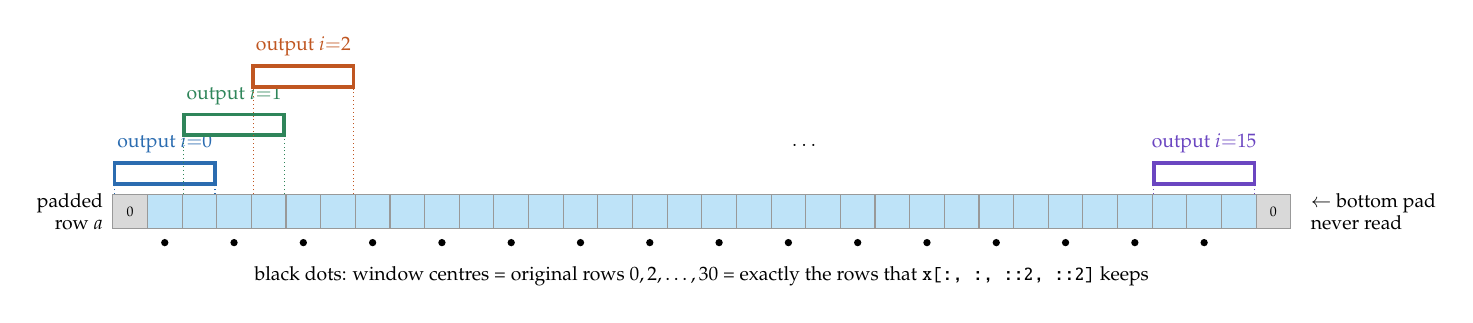
\begin{tikzpicture}[scale=0.44]
  \foreach \a in {0,...,33} {
    \pgfmathsetmacro{\col}{(\a==0 || \a==33) ? "black!15" : "c16"}
    \fill[\col] (\a,0) rectangle (\a+1,1); \draw[black!40] (\a,0) rectangle (\a+1,1);
  }
  \node[font=\tiny] at (0.5,0.5) {0}; \node[font=\tiny] at (33.5,0.5) {0};
  \node[left,font=\scriptsize,align=right] at (0,0.5) {padded\\row $a$};
  \foreach \i/\c/\h in {0/idea/1.3,1/repo/2.7,2/warn/4.1,15/shapec/1.3} {
    \pgfmathsetmacro{\s}{2*\i}
    \draw[\c,line width=1.3pt] (\s+0.05,\h) rectangle (\s+2.95,\h+0.6);
    \draw[\c,densely dotted] (\s+0.05,1) -- (\s+0.05,\h); \draw[\c,densely dotted] (\s+2.95,1) -- (\s+2.95,\h);
    \node[\c,font=\scriptsize,above] at (\s+1.5,\h+0.6) {output $i{=}\i$};
  }
  \node[font=\scriptsize] at (20,2.4) {$\cdots$};
  \node[right,font=\scriptsize,align=left] at (34.3,0.5) {$\leftarrow$ bottom pad\\never read};
  \foreach \a in {1,3,...,31} {\fill[black] (\a+0.5,-0.4) circle (3pt);}
  \node[below,font=\scriptsize] at (17,-0.8) {black dots: window centres = original rows $0,2,\dots,30$ = exactly the rows that \code{x[:, :, ::2, ::2]} keeps};
\end{tikzpicture}}
\end{center}

\begin{repo}[every convolution in the model]
All convolutions are \code{nn.Conv2d(..., kernel\_size=3, padding=1, bias=False)}. There are exactly three kinds:
\begin{center}
\begin{tabular}{@{}lccccr@{}}
\toprule
kind & $C_\text{in}\to C_\text{out}$ & $S$ & $H_\text{in}\to H_\text{out}$ & weight shape & \#weights\\
\midrule
stem & $3\to16$ & 1 & $32\to32$ & $(16,3,3,3)$ & 432\\
stage 1 (all 6) & $16\to16$ & 1 & $32\to32$ & $(16,16,3,3)$ & 2{,}304\\
stage 2, first & $16\to32$ & 2 & $32\to16$ & $(32,16,3,3)$ & 4{,}608\\
stage 2, other 5 & $32\to32$ & 1 & $16\to16$ & $(32,32,3,3)$ & 9{,}216\\
stage 3, first & $32\to64$ & 2 & $16\to8$ & $(64,32,3,3)$ & 18{,}432\\
stage 3, other 5 & $64\to64$ & 1 & $8\to8$ & $(64,64,3,3)$ & 36{,}864\\
\bottomrule
\end{tabular}
\end{center}
There is no $1{\times}1$ projection convolution anywhere. The shortcut has no parameters (\cref{sec:shortcut}). Depth changes in only three places: the stem ($3\to16$) and the first convolution of stages 2 and 3 ($16\to32$, $32\to64$), and each of those last two coincides with a stride-2 halving of the spatial size.
\end{repo}

\begin{warn}[why \texttt{bias=False}]
Every convolution is immediately followed by batch normalisation, which subtracts the per-channel mean. A per-channel conv bias would be subtracted right back out, so it would be a wasted parameter. BN's own shift $\beta$ plays the role of the bias.
\end{warn}

%-------------------------------------------------------------------
\subsection{Convolution \emph{is} a matrix multiplication (im2col)}
\label{sec:im2col}

\begin{idea}[unfold, multiply, fold]
For one image, cut out every $C_\text{in}\times K\times K$ window that the filter visits, flatten each to a column of length $C_\text{in}K^2$, and line the columns up:
\[
  X_\text{col} \in \R^{(C_\text{in}K^2)\times(H_\text{out}W_\text{out})}.
\]
Flatten each filter into a row: $W_\text{mat} = \mathcal W.\text{reshape}(C_\text{out},\,-1) \in \R^{C_\text{out}\times(C_\text{in}K^2)}$. Then the whole convolution is one matrix product
\[
  \underbrace{Y_\text{mat}}_{C_\text{out}\times H_\text{out}W_\text{out}} = \underbrace{W_\text{mat}}_{C_\text{out}\times C_\text{in}K^2}\;\underbrace{X_\text{col}}_{C_\text{in}K^2\times H_\text{out}W_\text{out}},
\]
and reshaping $Y_\text{mat}$ to $(C_\text{out},H_\text{out},W_\text{out})$ gives the output maps. The inner dimension $C_\text{in}K^2$ is ``one window'', and summing over it is exactly the triple sum in the boxed formula above.
\end{idea}

\begin{center}
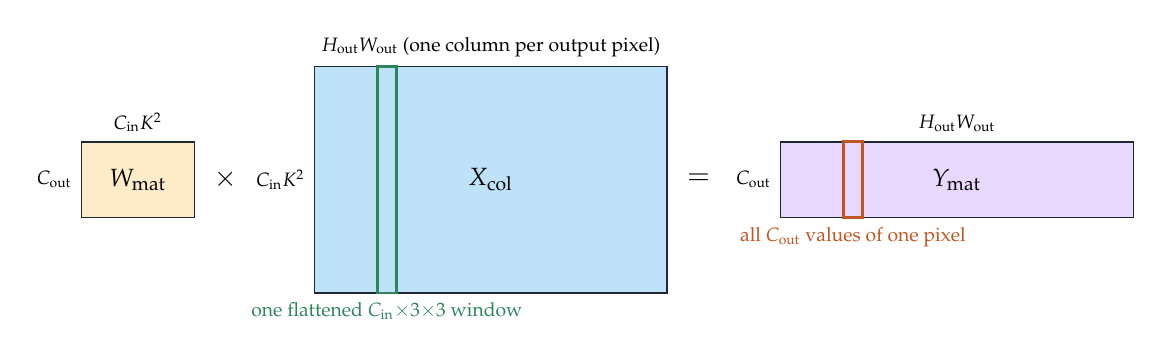
\begin{tikzpicture}[scale=0.8]
  \matr{0.6}{0.9}{1.8}{1.2}{cK}{$W_\text{mat}$}{$C_\text{out}$}{$C_\text{in}K^2$}
  \node at (2.9,1.5) {$\times$};
  \matr{4.3}{-0.3}{5.6}{3.6}{c16}{$X_\text{col}$}{$C_\text{in}K^2$}{$H_\text{out}W_\text{out}$ (one column per output pixel)}
  \node at (10.4,1.5) {$=$};
  \matr{11.7}{0.9}{5.6}{1.2}{cG}{$Y_\text{mat}$}{$C_\text{out}$}{$H_\text{out}W_\text{out}$}
  \draw[repo,line width=1pt] (5.3,-0.3) rectangle (5.6,3.3);
  \node[repo,font=\scriptsize,below] at (5.45,-0.3) {one flattened $C_\text{in}{\times}3{\times}3$ window};
  \draw[warn,line width=1pt] (12.7,0.9) rectangle (13.0,2.1);
  \node[warn,font=\scriptsize,below] at (12.85,0.9) {all $C_\text{out}$ values of one pixel};
\end{tikzpicture}
\end{center}

\begin{shapebox}[im2col sizes for this network, per image]
\begin{center}
\begin{tabular}{@{}lccc@{}}
\toprule
layer & $W_\text{mat}$ & $X_\text{col}$ & $Y_\text{mat}\to$ reshaped\\
\midrule
stem & $16\times 27$ & $27\times 1024$ & $16\times1024 \to (16,32,32)$\\
stage-1 conv & $16\times 144$ & $144\times 1024$ & $16\times 1024\to(16,32,32)$\\
stage-2 first conv ($S{=}2$) & $32\times 144$ & $144\times 256$ & $32\times256\to(32,16,16)$\\
stage-2 conv & $32\times 288$ & $288\times 256$ & $32\times 256\to(32,16,16)$\\
stage-3 first conv ($S{=}2$) & $64\times 288$ & $288\times 64$ & $64\times 64\to(64,8,8)$\\
stage-3 conv & $64\times 576$ & $576\times 64$ & $64\times64\to(64,8,8)$\\
\bottomrule
\end{tabular}
\end{center}
For the stem: $27 = 3\cdot3\cdot3$ (RGB $\times$ $3{\times}3$ window) and $1024 = 32\cdot32$ output pixels. For a batch, do this for each of the $N$ images (or concatenate their columns: $X_\text{col}$ becomes $C_\text{in}K^2\times N H_\text{out}W_\text{out}$).
\end{shapebox}

\begin{warn}[implementation vs.\ mathematics]
PyTorch on a GPU uses cuDNN, which picks among implicit-GEMM, Winograd and FFT algorithms and does not literally build $X_\text{col}$. The result is the same function up to floating-point rounding. Since the repo does not set \code{torch.backends.cudnn.deterministic}, two GPU runs with the same seed can differ in the last bits.
\end{warn}

\paragraph{Cost of a convolution.} Each output entry is a dot product of length $C_\text{in}K^2$, and there are $C_\text{out}H_\text{out}W_\text{out}$ entries, so a conv costs $C_\text{out}C_\text{in}K^2 H_\text{out}W_\text{out}$ multiply--adds (MACs) per image. A $16{\to}16$ conv at $32{\times}32$ costs $16\cdot16\cdot9\cdot1024 = 2{,}359{,}296$ MACs. A $32{\to}32$ conv at $16{\times}16$ costs $32\cdot32\cdot9\cdot256$, \emph{exactly the same number}, and so does $64{\to}64$ at $8{\times}8$. This is the ResNet design rule: \emph{when the feature map is halved, double the number of filters}, which keeps the time per layer constant.

%-------------------------------------------------------------------
\subsection{Batch normalisation}
\label{sec:bn}

\begin{idea}[normalise each channel over the batch, then re-scale]
For a 4-D activation $A\in\R^{N\times C\times H\times W}$, \code{BatchNorm2d(C)} treats each channel $c$ separately and pools statistics over the $m = N\cdot H\cdot W$ values of that channel:
\begin{align*}
  \mu_c &= \frac1m\sum_{n,h,w} A[n,c,h,w], &
  \sigma_c^2 &= \frac1m\sum_{n,h,w}\big(A[n,c,h,w]-\mu_c\big)^2, \\
  \hat A[n,c,h,w] &= \frac{A[n,c,h,w]-\mu_c}{\sqrt{\sigma_c^2+\varepsilon}}, &
  Y[n,c,h,w] &= \gamma_c\,\hat A[n,c,h,w] + \beta_c .
\end{align*}
$\gamma,\beta\in\R^{C}$ are learned and are broadcast as shape $(1,C,1,1)$. After normalisation each channel has mean 0 and variance $\approx1$ over the batch. $\gamma$ and $\beta$ then let the network choose any other scale and offset.
\end{idea}

\begin{center}
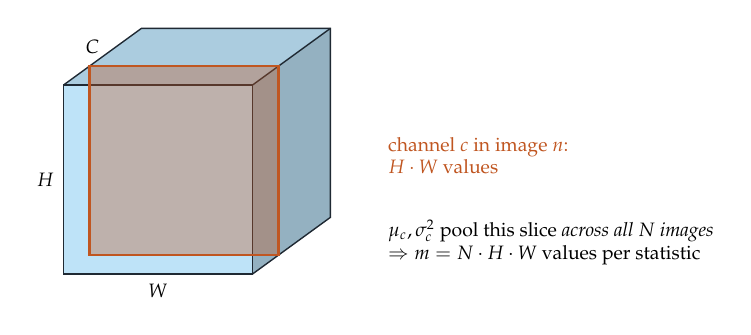
\begin{tikzpicture}
  \tensor{0}{0}{2.4}{2.4}{1.8}{c16}{$W$}{$H$}{$C$}
  % highlight one channel slice
  \pgfmathsetmacro{\o}{0.55*0.6}\pgfmathsetmacro{\p}{0.40*0.6}
  \fill[warn,opacity=0.35] (\o,\p) -- ++(2.4,0) -- ++(0,2.4) -- ++(-2.4,0) -- cycle;
  \draw[warn,thick] (\o,\p) rectangle ++(2.4,2.4);
  \node[warn,font=\scriptsize,align=left,right] at (4.0,1.5) {channel $c$ in image $n$:\\ $H\cdot W$ values};
  \node[font=\scriptsize,align=left,right] at (4.0,0.4) {$\mu_c,\sigma_c^2$ pool this slice \emph{across all $N$ images}\\ $\Rightarrow m=N\cdot H\cdot W$ values per statistic};
\end{tikzpicture}
\end{center}

\begin{repo}[PyTorch \texttt{BatchNorm2d} defaults, used as-is]
$\varepsilon = 10^{-5}$, \code{momentum} $\alpha=0.1$, \code{affine=True} ($\gamma$ initialised to 1, $\beta$ to 0), \code{track\_running\_stats=True}. Each BN layer therefore has $2C$ parameters and three buffers: \code{running\_mean} $\in\R^C$, \code{running\_var} $\in\R^C$, \code{num\_batches\_tracked} (an integer).

In \textbf{train mode} (\code{model.train()}), the batch statistics above are used, and the running buffers are updated after every forward pass:
\[
  r_\mu \leftarrow (1-\alpha)\,r_\mu + \alpha\,\mu_c, \qquad
  r_{\sigma^2} \leftarrow (1-\alpha)\,r_{\sigma^2} + \alpha\,\tfrac{m}{m-1}\,\sigma_c^2 .
\]
Note the asymmetry. The \emph{normalisation} uses the biased variance ($\div m$), while the \emph{running estimate} stores the unbiased one ($\div(m-1)$).

In \textbf{eval mode} (\code{model.eval()}), the batch is ignored and the running buffers are used. BN then becomes a fixed per-channel affine map (\cref{sec:evalbn}).

How many values each statistic pools, for a full batch of 128 images:
\begin{center}
\begin{tabular}{@{}lcr@{}}
\toprule
where & activation shape & $m=N H W$\\
\midrule
stem BN and stage 1 & $(128,16,32,32)$ & $131{,}072$\\
stage 2 & $(128,32,16,16)$ & $32{,}768$\\
stage 3 & $(128,64,8,8)$ & $8{,}192$\\
\bottomrule
\end{tabular}
\end{center}
The last batch of each epoch is smaller (80 images on 50k, 72 on 45k), so its statistics are noisier, but $m$ is still in the thousands.
\end{repo}

\begin{warn}[forward hooks and \texttt{model.train()}]
Because BN updates its running buffers on \emph{every} forward pass in train mode, even under \code{torch.no\_grad()}, a forward pass in the wrong mode changes the model. \file{scripts/check\_eval.py} tests exactly this: it runs 20 no-grad forward passes in train mode and then calls \code{evaluate}. \code{evaluate()} and \code{predict()} both call \code{model.eval()} first, and \code{train\_one\_epoch} calls \code{model.train()} first, so the training loop always switches modes correctly.
\end{warn}

%-------------------------------------------------------------------
\subsection{ReLU}
\label{sec:relu}

\begin{idea}
$\ReLU(z) = \max(0,z)$, element-wise, shape-preserving. Its derivative is $\mathbb 1[z>0]$ (PyTorch uses 0 at exactly $z=0$). It is the only non-linearity in the network.
\end{idea}

\begin{repo}
One \code{nn.ReLU()} module per \code{BasicBlock} (used twice in \code{forward}), and one in \code{ResNetCIFAR} after the stem. Re-using one module object twice is safe because ReLU has no parameters or state. The \code{inplace} flag is left at its default \code{False}.
\end{repo}

%-------------------------------------------------------------------
\subsection{Global average pooling and flatten}
\label{sec:gap}

\begin{idea}
\code{nn.AdaptiveAvgPool2d(1)} picks its window so that the output is $1\times1$. On an $8\times8$ input that window is the whole map:
\[
  p[n,c] \;=\; \frac{1}{64}\sum_{h=0}^{7}\sum_{w=0}^{7} A[n,c,h,w], \qquad (N,64,8,8)\;\longrightarrow\;(N,64,1,1).
\]
\code{nn.Flatten(1,-1)} then merges axes 1--3: $(N,64,1,1)\to(N,64)$. It has no parameters and only changes the view.
\end{idea}

\begin{center}
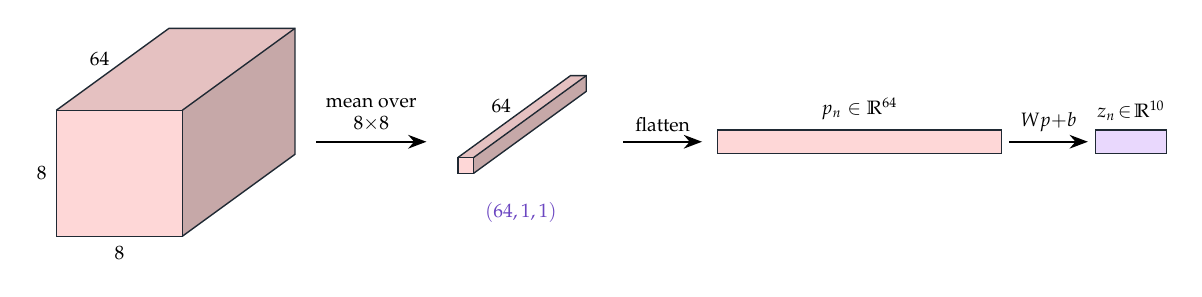
\begin{tikzpicture}
  \tensor{0}{0}{1.6}{1.6}{2.6}{c64}{$8$}{$8$}{$64$}
  \draw[-{Stealth},thick] (3.3,1.2) -- (4.7,1.2) node[midway,above,font=\scriptsize,align=center]{mean over\\$8{\times}8$};
  \tensor{5.1}{0.8}{0.2}{0.2}{2.6}{c64}{}{}{$64$}
  \node[font=\scriptsize] at (5.9,0.3) {\shp{64,1,1}};
  \draw[-{Stealth},thick] (7.2,1.2) -- (8.2,1.2) node[midway,above,font=\scriptsize]{flatten};
  \matr{8.4}{1.05}{3.6}{0.3}{c64}{}{}{$p_n\in\R^{64}$}
  \draw[-{Stealth},thick] (12.1,1.2) -- (13.1,1.2) node[midway,above,font=\scriptsize]{$Wp{+}b$};
  \matr{13.2}{1.05}{0.9}{0.3}{cG}{}{}{$z_n\!\in\!\R^{10}$}
\end{tikzpicture}
\end{center}

\begin{repo}
Pooling throws away \emph{where} a feature fired and keeps only \emph{how strongly on average}. That is why the classifier needs just $64\times10$ weights rather than $64\cdot8\cdot8\times10 = 40{,}960$. There is no max-pooling anywhere in the network: downsampling is done only by stride-2 convolutions.
\end{repo}

%-------------------------------------------------------------------
\subsection{Logits, softmax, cross-entropy and class selection}
\label{sec:ce}

\begin{idea}[from scores to a loss]
The model outputs \emph{logits} $z\in\R^{10}$ per image: unnormalised scores, any real numbers. Softmax turns them into a probability vector:
\[
  s_k = \softmax(z)_k = \frac{e^{z_k}}{\sum_{j=0}^{9} e^{z_j}}, \qquad s_k>0,\quad \sum_k s_k = 1 .
\]
Adding the same constant to every logit leaves $s$ unchanged ($e^{z_k+c}/\sum e^{z_j+c}$). Libraries exploit this to stay numerically stable, using $\log s_k = z_k - \operatorname{logsumexp}(z)$ with $\operatorname{logsumexp}(z) = M + \log\sum_j e^{z_j-M}$, $M=\max_j z_j$.

The cross-entropy loss for one example with true class $y$ is the negative log-probability of the correct class:
\[
  \ell(z,y) = -\log s_y = \operatorname{logsumexp}(z) - z_y ,
\]
and over a batch (PyTorch's default \code{reduction='mean'}):
\[
  \mathcal L = \frac1N\sum_{n=1}^{N}\ell(z_n,y_n).
\]
If the network is uninformed and outputs equal logits, $s_k = 1/10$ and $\ell = \ln 10 \approx 2.3026$. That is the loss to expect at initialisation.

\textbf{Class selection.} The predicted class is $\hat y = \argmax_k z_k = \argmax_k s_k$. Softmax is monotonic, so it is not needed to pick the class, only to report a probability.
\end{idea}

\begin{repo}[three places that turn logits into decisions]
\begin{itemize}[nosep]
  \item \textbf{Training/eval loss:} \code{nn.CrossEntropyLoss()} takes \emph{raw logits} $(N,10)$ and \code{int64} targets $(N,)$. Internally it is \code{log\_softmax} followed by negative log-likelihood. The model therefore has no softmax layer: putting one in would apply softmax twice.
  \item \textbf{Accuracy:} \code{torch.argmax(logits, dim=1) == label} in \code{train\_one\_epoch} and \code{evaluate}. \code{dim=1} is the class axis, giving shape $(N,)$.
  \item \textbf{Probabilities:} \code{torch.softmax(logits, dim=1)} in \code{predict()} (evaluation report) and in the service, which then takes \code{torch.topk(probs, 3)} and returns the three largest $(s_k, k)$ pairs.
\end{itemize}
\end{repo}

\section{One residual block in full detail}
\label{sec:block}

\subsection{The idea: learn a correction, not a whole mapping}

\begin{idea}[residual learning]
A stack of layers is asked to represent some mapping $\mathcal H(x)$. A residual block instead computes
\[
  y \;=\; \ReLU\big(\mathcal F(x) + s(x)\big),
\]
where $\mathcal F$ is a small stack of layers (the \emph{residual branch}) and $s$ is a \emph{shortcut} that is the identity whenever shapes allow. The branch only has to learn the difference $\mathcal F = \mathcal H - x$. If the best thing a block can do is ``nothing'', it only has to drive $\mathcal F$ towards zero, which is easy (shrink the last BN's $\gamma$). A plain stack has to learn an exact identity through two ReLU-convolutions, which is hard. He et al.\ argue that this is why deep plain networks \emph{train} worse (higher training error), not just generalise worse. This repo's ablation reproduces that effect (\cref{sec:ablation}).
\end{idea}

\subsection{The code}

\begin{lstlisting}[firstnumber=6]
class BasicBlock(nn.Module):
    def __init__(self,in_ch,out_ch,stride,residual):
        super().__init__()
        ...
        self.first_conv = nn.Conv2d(bias=False,in_channels=in_ch,out_channels=out_ch,stride=stride,padding=1,kernel_size=3)
        self.bn1 = nn.BatchNorm2d(out_ch)
        self.relu = nn.ReLU()
        self.second_conv = nn.Conv2d(bias=False,in_channels=out_ch,out_channels=out_ch,stride=1,padding=1,kernel_size=3)
        self.bn2 = nn.BatchNorm2d(out_ch)
        self.downsampling_need = False
        if residual:
            if (stride != 1) or (in_ch != out_ch):
                self.downsampling_need = True
    def forward(self,x):
        f = self.first_conv(x)
        f = self.bn1(f)
        f = self.relu(f)
        f = self.second_conv(f)
        f = self.bn2(f)
        if self.residual:
            if self.downsampling_need:
                x = x[:,:,::2,::2]
                pads = (self.out_ch - self.in_ch) // 2
                x = F.pad(x, (0, 0, 0, 0, pads, pads))
            x = x + f
        else:
            x = f
        x = self.relu(x)
        return x
\end{lstlisting}

\subsection{The block as equations}

\begin{repo}[exact forward computation of \texttt{BasicBlock}]
With $\mathcal W_1\in\R^{C_\text{out}\times C_\text{in}\times3\times3}$ (stride $S$), $\mathcal W_2\in\R^{C_\text{out}\times C_\text{out}\times3\times3}$ (stride 1) and BN parameters $(\gamma_1,\beta_1)$, $(\gamma_2,\beta_2)\in\R^{C_\text{out}}$:
\begin{alignat*}{2}
  a_1 &= \conv_{S}(x;\mathcal W_1) &&\qquad\text{\small first conv: may halve $H,W$, may change depth}\\
  b_1 &= \BN_{\gamma_1,\beta_1}(a_1)\\
  r_1 &= \ReLU(b_1)\\
  a_2 &= \conv_{1}(r_1;\mathcal W_2) &&\qquad\text{\small second conv: shape preserved}\\
  \mathcal F(x) = b_2 &= \BN_{\gamma_2,\beta_2}(a_2) &&\qquad\text{\small no ReLU yet}
\end{alignat*}
\[
  s(x) = \begin{cases}
    x & \text{residual, } S=1,\ C_\text{in}=C_\text{out}\\
    \operatorname{pad}_\text{ch}\!\big(x[:,:,::2,::2]\big) & \text{residual, } S=2 \text{ or } C_\text{in}\neq C_\text{out}\\
    0 & \text{plain (\code{residual=False})}
  \end{cases}
\]
\[
  \boxed{\,y = \ReLU\big(\mathcal F(x) + s(x)\big)\,}
\]
The ReLU comes \emph{after} the addition. This is the original ``post-activation'' ResNet v1 block of the 2015 paper, not the 2016 pre-activation variant.
\end{repo}

\subsection{Identity block: 16 channels in, 16 out, stride 1}
\label{sec:idblock}

This is every block of stage 1, and blocks 2--3 of stages 2 and 3 with their own widths.

\begin{center}
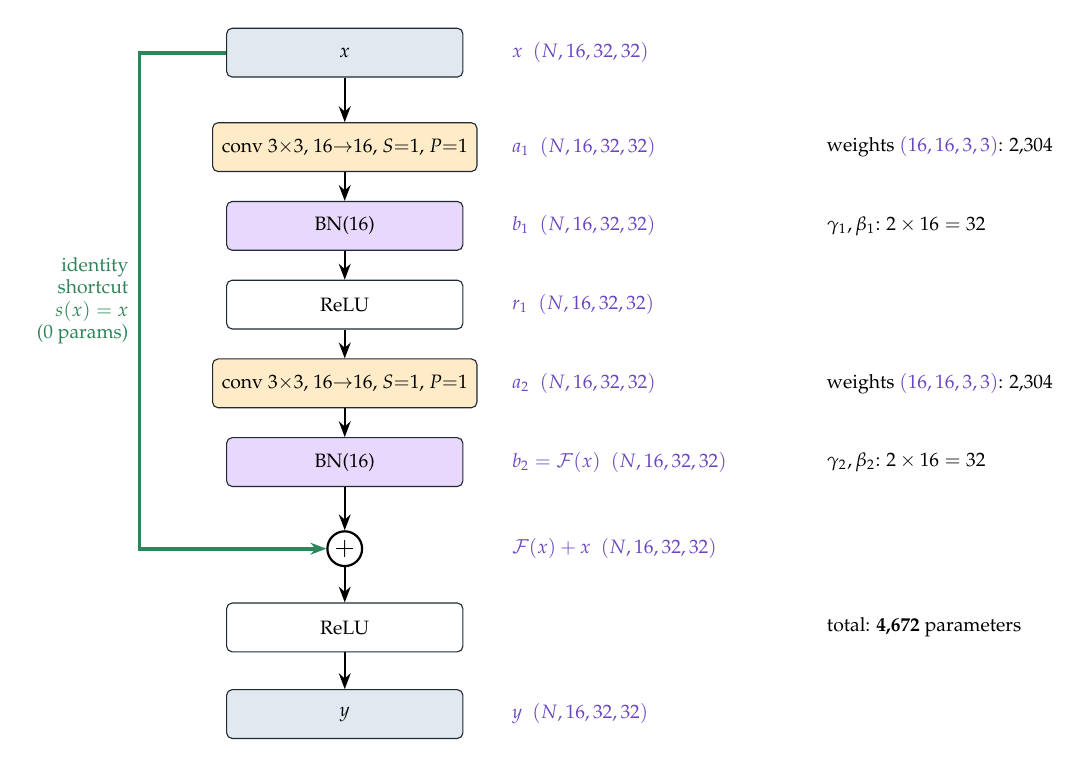
\begin{tikzpicture}[
  op/.style={draw=ink,rounded corners=2pt,fill=#1,font=\scriptsize,minimum width=3.0cm,minimum height=0.62cm,align=center},
  op/.default=white,
  ar/.style={-{Stealth[length=2mm]},thick}]
  \node[op=cIn] (x) at (0,0) {$x$};
  \node[op=cK]  (c1) at (0,-1.2) {conv $3{\times}3$, $16{\to}16$, $S{=}1$, $P{=}1$};
  \node[op=cG]  (b1) at (0,-2.2) {BN(16)};
  \node[op]     (r1) at (0,-3.2) {ReLU};
  \node[op=cK]  (c2) at (0,-4.2) {conv $3{\times}3$, $16{\to}16$, $S{=}1$, $P{=}1$};
  \node[op=cG]  (b2) at (0,-5.2) {BN(16)};
  \node[circle,draw,thick,inner sep=1pt,font=\small] (add) at (0,-6.3) {$+$};
  \node[op]     (r2) at (0,-7.3) {ReLU};
  \node[op=cIn] (y) at (0,-8.4) {$y$};
  \draw[ar] (x) -- (c1); \draw[ar] (c1) -- (b1); \draw[ar] (b1) -- (r1); \draw[ar] (r1) -- (c2); \draw[ar] (c2) -- (b2); \draw[ar] (b2) -- (add); \draw[ar] (add) -- (r2); \draw[ar] (r2) -- (y);
  \draw[ar,repo,line width=1.4pt] (x.west) -- ++(-1.1,0) |- (add.west) node[pos=0.25,left,font=\scriptsize,align=right]{identity\\shortcut\\$s(x)=x$\\(0 params)};
  % shapes on the right
  \foreach \yy/\lab in {0/{$x$}, -1.2/{$a_1$}, -2.2/{$b_1$}, -3.2/{$r_1$}, -4.2/{$a_2$}, -5.2/{$b_2=\mathcal F(x)$}, -6.3/{$\mathcal F(x)+x$}, -8.4/{$y$}} {
    \node[right,font=\scriptsize,shapec] at (2.0,\yy) {\lab\; \shp{N,16,32,32}};
  }
  \node[right,font=\scriptsize] at (6.0,-1.2) {weights \shp{16,16,3,3}: 2{,}304};
  \node[right,font=\scriptsize] at (6.0,-2.2) {$\gamma_1,\beta_1$: $2\times16=32$};
  \node[right,font=\scriptsize] at (6.0,-4.2) {weights \shp{16,16,3,3}: 2{,}304};
  \node[right,font=\scriptsize] at (6.0,-5.2) {$\gamma_2,\beta_2$: $2\times16=32$};
  \node[right,font=\scriptsize] at (6.0,-7.3) {total: \textbf{4{,}672} parameters};
\end{tikzpicture}
\end{center}

\begin{shapebox}[identity block, worked]
Input \shp{128,16,32,32}. First conv: $H_\text{out}=\lfloor(32+2-3)/1\rfloor+1=32$, depth $=$ number of filters $=16$, so \shp{128,16,32,32}. BN and ReLU preserve shape. Second conv: same arithmetic, \shp{128,16,32,32}. The shortcut is $x$ itself, \shp{128,16,32,32}, so the addition is element-wise with no broadcasting (shapes identical). The output is \shp{128,16,32,32}. In im2col form, each conv is $(16\times144)\cdot(144\times1024)$ per image, i.e.\ $2.36$M MACs.
\end{shapebox}

\subsection{Downsampling block: 16 channels in, 32 out, stride 2}
\label{sec:shortcut}

This is the first block of stage 2 (and, with $32\to64$ and $16\to8$, the first block of stage 3). Here the two branches would not have the same shape unless the shortcut does something.

\begin{center}
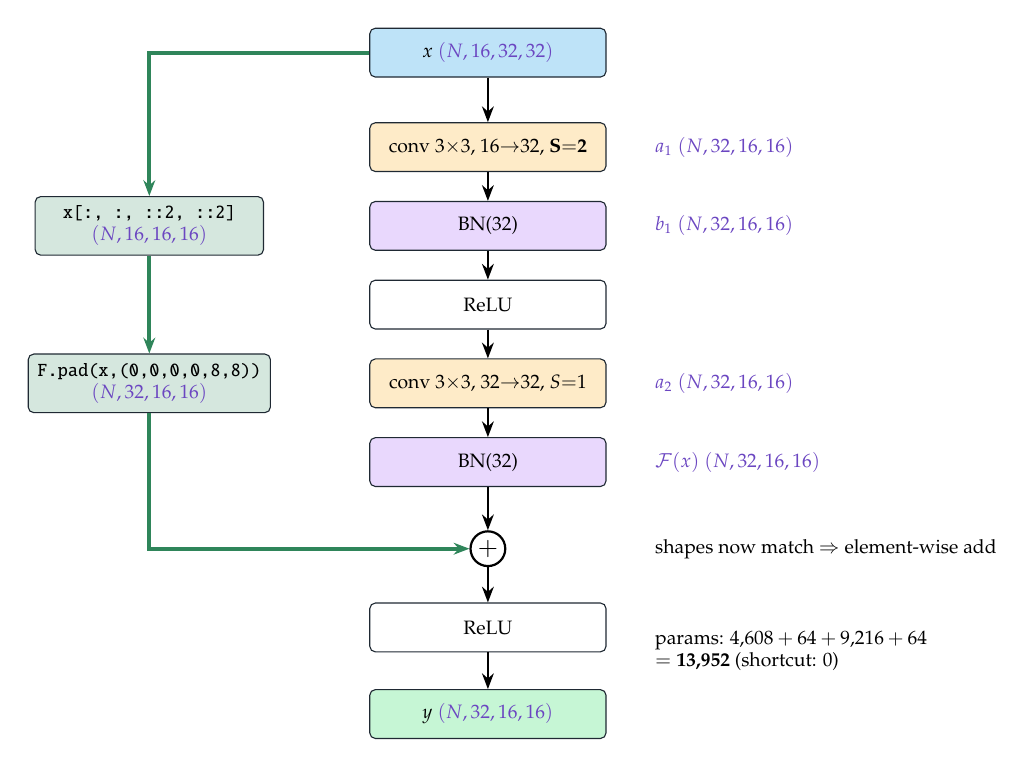
\begin{tikzpicture}[
  op/.style={draw=ink,rounded corners=2pt,fill=#1,font=\scriptsize,minimum width=3.0cm,minimum height=0.62cm,align=center},
  op/.default=white,
  ar/.style={-{Stealth[length=2mm]},thick}]
  \node[op=c16] (x) at (0,0) {$x$ \shp{N,16,32,32}};
  \node[op=cK]  (c1) at (0,-1.2) {conv $3{\times}3$, $16{\to}32$, $\mathbf{S{=}2}$};
  \node[op=cG]  (b1) at (0,-2.2) {BN(32)};
  \node[op]     (r1) at (0,-3.2) {ReLU};
  \node[op=cK]  (c2) at (0,-4.2) {conv $3{\times}3$, $32{\to}32$, $S{=}1$};
  \node[op=cG]  (b2) at (0,-5.2) {BN(32)};
  \node[circle,draw,thick,inner sep=1pt,font=\small] (add) at (0,-6.3) {$+$};
  \node[op]     (r2) at (0,-7.3) {ReLU};
  \node[op=c32] (y) at (0,-8.4) {$y$ \shp{N,32,16,16}};
  \draw[ar] (x) -- (c1); \draw[ar] (c1) -- (b1); \draw[ar] (b1) -- (r1); \draw[ar] (r1) -- (c2); \draw[ar] (c2) -- (b2); \draw[ar] (b2) -- (add); \draw[ar] (add) -- (r2); \draw[ar] (r2) -- (y);
  \node[op=repo!20,minimum width=2.9cm] (sub) at (-4.3,-2.2) {\code{x[:, :, ::2, ::2]}\\ \shp{N,16,16,16}};
  \node[op=repo!20,minimum width=2.9cm] (pad) at (-4.3,-4.2) {\code{F.pad(x,(0,0,0,0,8,8))}\\ \shp{N,32,16,16}};
  \draw[ar,repo,line width=1.4pt] (x.west) -| (sub.north);
  \draw[ar,repo,line width=1.4pt] (sub) -- (pad);
  \draw[ar,repo,line width=1.4pt] (pad.south) |- (add.west);
  \foreach \yy/\lab in {-1.2/{$a_1$ \shp{N,32,16,16}}, -2.2/{$b_1$ \shp{N,32,16,16}}, -4.2/{$a_2$ \shp{N,32,16,16}}, -5.2/{$\mathcal F(x)$ \shp{N,32,16,16}}} {
    \node[right,font=\scriptsize,shapec] at (2.0,\yy) {\lab};
  }
  \node[right,font=\scriptsize] at (2.0,-6.3) {shapes now match $\Rightarrow$ element-wise add};
  \node[right,font=\scriptsize,align=left] at (2.0,-7.6) {params: $4{,}608 + 64 + 9{,}216 + 64$\\$=\textbf{13{,}952}$ (shortcut: 0)};
\end{tikzpicture}
\end{center}

\paragraph{Step 1: spatial subsampling.} \code{x[:,:,::2,::2]} keeps rows $0,2,4,\dots,30$ and columns $0,2,\dots,30$:
\[
  x_\text{sub}[n,c,i,j] = x[n,c,2i,2j], \qquad \shp{N,16,32,32}\to\shp{N,16,16,16}.
\]
Three quarters of the positions are dropped (no averaging). As shown in \cref{sec:conv}, the stride-2 convolution of the main branch centres its windows on the same even positions $(2i,2j)$, so output pixel $(i,j)$ of the branch and of the shortcut describe the same place in the image.

\paragraph{Step 2: channel zero-padding.} \code{F.pad}'s padding tuple is read \emph{from the last axis backwards} in pairs: $(\text{left},\text{right})$ of $W$, then $(\text{top},\text{bottom})$ of $H$, then $(\text{front},\text{back})$ of the channel axis. So \code{(0,0,0,0,8,8)} leaves $W$ and $H$ alone and adds 8 all-zero channels \emph{before} and 8 \emph{after} the existing 16. Here \code{pads = (32-16)//2 = 8}; for stage 3 it is \code{(64-32)//2 = 16}.

\begin{center}
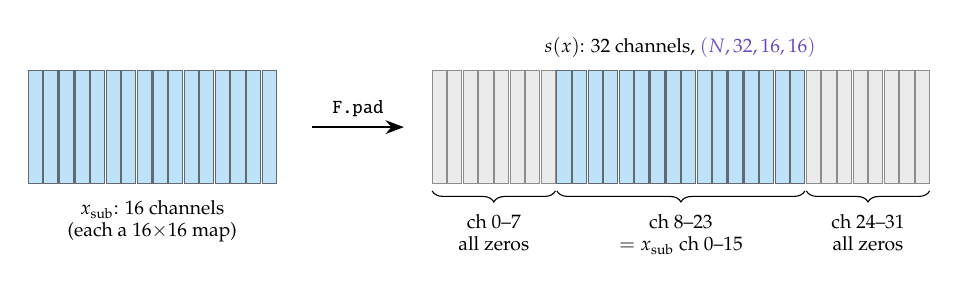
\begin{tikzpicture}[scale=0.9]
  % channels drawn as a row of thin strips (one strip = one 16x16 map seen edge-on)
  \foreach \c in {0,...,15} { \fill[c16,draw=ink!70] (0.22*\c,0) rectangle ++(0.2,1.6); }
  \node[font=\scriptsize,below,align=center] at (1.75,-0.1) {$x_\text{sub}$: 16 channels\\(each a $16{\times}16$ map)};
  \draw[-{Stealth},thick] (4.0,0.8) -- (5.3,0.8) node[midway,above,font=\scriptsize]{\code{F.pad}};
  \begin{scope}[shift={(5.7,0)}]
  \foreach \c in {0,...,31} {
    \pgfmathtruncatemacro{\isz}{(\c<8 || \c>23) ? 1 : 0}
    \ifnum\isz=1 \fill[black!8,draw=black!45] (0.22*\c,0) rectangle ++(0.2,1.6);
    \else \fill[c16,draw=ink!70] (0.22*\c,0) rectangle ++(0.2,1.6); \fi
  }
  \draw[decorate,decoration={brace,amplitude=4pt,mirror}] (0,-0.1) -- (1.74,-0.1) node[midway,below=5pt,font=\scriptsize,align=center]{ch 0--7\\all zeros};
  \draw[decorate,decoration={brace,amplitude=4pt,mirror}] (1.76,-0.1) -- (5.26,-0.1) node[midway,below=5pt,font=\scriptsize,align=center]{ch 8--23\\$=x_\text{sub}$ ch 0--15};
  \draw[decorate,decoration={brace,amplitude=4pt,mirror}] (5.28,-0.1) -- (7.02,-0.1) node[midway,below=5pt,font=\scriptsize,align=center]{ch 24--31\\all zeros};
  \node[font=\scriptsize,above] at (3.5,1.65) {$s(x)$: 32 channels, \shp{N,32,16,16}};
  \end{scope}
\end{tikzpicture}
\end{center}
\[
  s(x)[n,c,i,j] =
  \begin{cases}
    x[n,\,c-8,\,2i,\,2j] & 8\le c\le 23\\
    0 & \text{otherwise}
  \end{cases}
\]
\[
  \Longrightarrow\qquad y[n,c] = \ReLU\big(\mathcal F(x)[n,c] + s(x)[n,c]\big).
\]
Output channels 0--7 and 24--31 receive \emph{only} the residual branch. Channels 8--23 receive branch $+$ old features.

\begin{repo}[verified on the trained model]
Feeding \file{samples/test0.png} through the trained network and inspecting the first block of stage 2: \code{s(x)} has shape \shp{1,32,16,16}, channels 0--7 and 24--31 are exactly zero, channels 8--23 are not, and recomputing $\ReLU(\mathcal F(x)+s(x))$ by hand matches \code{stage2[0](x)} with maximum difference $0.0$.
\end{repo}

\begin{warn}[``option A'' vs.\ the alternatives]
The paper describes three shortcut options. (A) Zero-padding for increasing dimensions, parameter-free. (B) $1{\times}1$ projection convolutions only where dimensions change. (C) Projections everywhere. For the CIFAR-10 networks the paper says ``we use identity shortcuts in all cases (i.e., option A)'', and this repo follows that, so the shortcut adds \textbf{zero parameters} and the plain and residual models have \emph{identical} parameter counts (269{,}722 each for $n=3$). The paper does not specify which side the zero channels go on. This repo pads symmetrically (8 before, 8 after), a common choice in public reimplementations; padding only at the end would be equally valid. The subsampling takes every other pixel; it is not average pooling.
\end{warn}

\subsection{The plain block}

\begin{repo}[\texttt{residual=False}, used by \texttt{--plain}]
The branch is identical, but \code{x = f} replaces \code{x = x + f}, so $y=\ReLU(\mathcal F(x))$. There is no shortcut, \code{downsampling\_need} stays \code{False}, and the subsample/pad code never runs. Shapes still work because the first convolution alone handles both the stride and the channel change. Same layers, same parameters, same FLOPs: the only difference between ``plain-20'' and ``ResNet-20'' is the $+\,s(x)$. That is what makes the ablation a clean experiment.
\end{repo}

\subsection{Why the shortcut helps optimisation (the one-line gradient argument)}
\label{sec:whyres}

\begin{idea}
Ignore the final ReLU for a moment, so a block is $y = x + \mathcal F(x)$. Its Jacobian is
\[
  \dd{y}{x} = I + \dd{\mathcal F}{x}.
\]
Back-propagating through $L$ stacked identity blocks multiplies these:
\[
  \dd{\mathcal L}{x_0} \;=\; \dd{\mathcal L}{x_L}\prod_{l=1}^{L}\Big(I + \dd{\mathcal F_l}{x_{l-1}}\Big)
  \;=\; \dd{\mathcal L}{x_L}\Big(I + \sum_l \dd{\mathcal F_l}{x_{l-1}} + \cdots\Big).
\]
The expansion always contains the bare term $\partial\mathcal L/\partial x_L$, so the gradient reaches early layers unchanged by any weight matrix. In a plain network the gradient is $\prod_l \partial\mathcal F_l/\partial x_{l-1}$, a product of $L$ Jacobians, with no such guaranteed path. The real block has a ReLU after the add, which zeroes the gradient where $y=0$; this weakens the argument but does not remove the path. BN keeps each $\partial\mathcal F/\partial x$ well scaled. This is a sketch of the intuition, not a proof. The ablation (plain-56 has \emph{higher training error} than plain-20, while res-56 beats res-20) is the empirical evidence.
\end{idea}

\subsection{Activations in a real block}

\begin{repo}[block \texttt{stage1.0} on \texttt{samples/test0.png}, trained model, eval mode]
\begin{center}
\small
\begin{tabular}{@{}lcrrrr@{}}
\toprule
tensor & shape & mean & std & min & max\\
\midrule
input $x$ (output of stem ReLU) & \shp{1,16,32,32} & 0.439 & 0.513 & 0.00 & 3.65 \\
$a_1$ = first conv & \shp{1,16,32,32} & $-0.325$ & 2.130 & $-9.15$ & 5.72\\
$b_1$ = BN1 & \shp{1,16,32,32} & 0.090 & 0.806 & $-3.52$ & 3.29\\
$a_2$ = second conv (after ReLU) & \shp{1,16,32,32} & 0.035 & 1.493 & $-8.37$ & 7.26\\
$\mathcal F(x)=b_2$ = BN2 & \shp{1,16,32,32} & 0.044 & 0.656 & $-3.52$ & 3.15\\
$y=\ReLU(\mathcal F(x)+x)$ & \shp{1,16,32,32} & 0.615 & 0.682 & 0.00 & 5.31\\
\bottomrule
\end{tabular}
\end{center}
The convolution outputs have a large spread (std $\approx 2$), and BN brings each channel back to std $\lesssim 1$ before the next non-linearity. 25.6\% of the block's outputs are exactly zero after the final ReLU. The residual branch $\mathcal F(x)$ is small compared with the running signal: its std is $0.66$, while the output's mean is $0.62$. This is the ``small correction'' picture of residual learning, measured.
\end{repo}

\section{The complete ResNet-20 and its shape flow}
\label{sec:arch}

\subsection{The $6n+2$ family}

\begin{idea}[counting layers]
The CIFAR ResNets of the paper consist of a $3{\times}3$ stem convolution, then three \emph{stages} of $n$ basic blocks each, at feature-map sizes $32$, $16$, $8$ with $16$, $32$, $64$ filters, then global average pooling and a 10-way fully connected layer. Each block holds 2 weighted layers, so
\[
  \underbrace{1}_{\text{stem}} + \underbrace{3\cdot n\cdot 2}_{\text{blocks}} + \underbrace{1}_{\text{FC}} = 6n+2 \text{ weighted layers.}
\]
$n=3$ gives 20 and $n=9$ gives 56. BN, ReLU and pooling are not counted as layers. Only layers with weights are.
\end{idea}

\begin{repo}[\texttt{ResNetCIFAR(n, residual=True, num\_classes=10, in\_channels=3, widths=(16,32,64))}]
\begin{lstlisting}[firstnumber=45]
        self.stem = nn.Conv2d(bias=False,stride=1,padding=1,kernel_size=3,in_channels=in_channels,out_channels=self.widths[0])
        self.bn1 = nn.BatchNorm2d(self.widths[0])
        self.relu = nn.ReLU()
        self.linear = nn.Linear(self.widths[2],self.num_classes)
        self.avg_pool = nn.AdaptiveAvgPool2d(1)
        self.flatten = nn.Flatten(1,-1)
        self.stage1 = self._make_stage(in_ch=widths[0],out_ch=widths[0],stride=1)
        self.stage2 = self._make_stage(in_ch=widths[0],out_ch=widths[1],stride=2)
        self.stage3 = self._make_stage(in_ch=widths[1],out_ch=widths[2],stride=2)
        self._init_weights()
    def _make_stage(self,in_ch,out_ch,stride):
        blocks = []
        blocks.append(BasicBlock(in_ch=in_ch,out_ch=out_ch,stride=stride,residual=self.residual))
        for i in range(self.n - 1):
            blocks.append(BasicBlock(in_ch=out_ch,out_ch=out_ch,stride=1,residual=self.residual))
        return nn.Sequential(*blocks)
\end{lstlisting}
Only the \emph{first} block of a stage gets the stage's stride and the channel change; the other $n-1$ are identity blocks. Stage 1 has stride 1 and $16\to16$, so all its blocks are identity blocks and there is no downsampling at the start. The forward pass is the straight composition
\[
  z = \text{Linear}\Big(\text{Flatten}\big(\text{GAP}(\text{stage}_3(\text{stage}_2(\text{stage}_1(\ReLU(\BN(\text{stem}(x)))))))\big)\Big).
\]
\end{repo}

\subsection{The shape flow, drawn}

\begin{center}
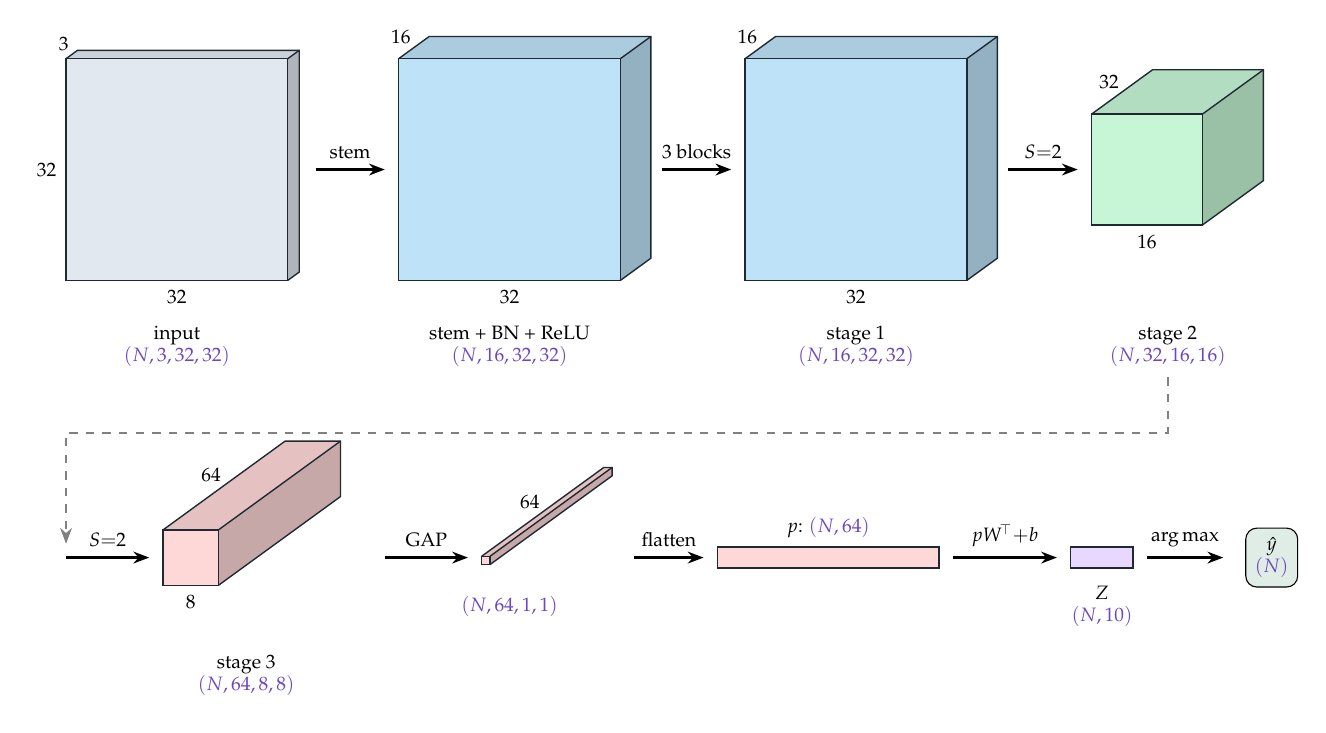
\begin{tikzpicture}[scale=0.88,ar/.style={-{Stealth[length=2mm]},thick}]
  % row 1
  \tensor{0}{0}{3.2}{3.2}{0.3}{cIn}{$32$}{$32$}{$3$}
  \node[font=\scriptsize,align=center] at (1.6,-0.95) {input\\\shp{N,3,32,32}};
  \draw[ar] (3.6,1.6) -- (4.6,1.6) node[midway,above,font=\scriptsize]{stem};
  \tensor{4.8}{0}{3.2}{3.2}{0.8}{c16}{$32$}{}{$16$}
  \node[font=\scriptsize,align=center] at (6.4,-0.95) {stem + BN + ReLU\\\shp{N,16,32,32}};
  \draw[ar] (8.6,1.6) -- (9.6,1.6) node[midway,above,font=\scriptsize]{$3$ blocks};
  \tensor{9.8}{0}{3.2}{3.2}{0.8}{c16}{$32$}{}{$16$}
  \node[font=\scriptsize,align=center] at (11.4,-0.95) {stage 1\\\shp{N,16,32,32}};
  \draw[ar] (13.6,1.6) -- (14.6,1.6) node[midway,above,font=\scriptsize]{$S{=}2$};
  \tensor{14.8}{0.8}{1.6}{1.6}{1.6}{c32}{$16$}{}{$32$}
  \node[font=\scriptsize,align=center] at (15.9,-0.95) {stage 2\\\shp{N,32,16,16}};
  % row 2
  \begin{scope}[shift={(0,-5.2)}]
  \draw[ar] (0,1.2) -- (1.2,1.2) node[midway,above,font=\scriptsize]{$S{=}2$};
  \tensor{1.4}{0.8}{0.8}{0.8}{3.2}{c64}{$8$}{}{$64$}
  \node[font=\scriptsize,align=center] at (2.6,-0.5) {stage 3\\\shp{N,64,8,8}};
  \draw[ar] (4.6,1.2) -- (5.8,1.2) node[midway,above,font=\scriptsize]{GAP};
  \tensor{6.0}{1.1}{0.12}{0.12}{3.2}{c64}{}{}{$64$}
  \node[font=\scriptsize,align=center] at (6.4,0.5) {\shp{N,64,1,1}};
  \draw[ar] (8.2,1.2) -- (9.2,1.2) node[midway,above,font=\scriptsize]{flatten};
  \matr{9.4}{1.05}{3.2}{0.3}{c64}{}{}{$p$: \shp{N,64}}
  \draw[ar] (12.8,1.2) -- (14.3,1.2) node[midway,above,font=\scriptsize]{$pW\T{+}b$};
  \matr{14.5}{1.05}{0.9}{0.3}{cG}{}{}{}
  \node[font=\scriptsize,align=center] at (14.95,0.5) {$Z$\\\shp{N,10}};
  \draw[ar] (15.6,1.2) -- (16.7,1.2) node[midway,above,font=\scriptsize]{$\argmax$};
  \node[draw,rounded corners,font=\scriptsize,fill=repo!15,align=center] at (17.4,1.2) {$\hat y$\\\shp{N}};
  \end{scope}
  \draw[ar,dashed,black!50] (15.9,-1.4) -- (15.9,-2.2) -- (0,-2.2) -- (0,-3.8);
\end{tikzpicture}
\end{center}

Read it as two trends running in opposite directions. The spatial size halves twice ($32\to16\to8$) and the depth doubles twice ($16\to32\to64$). The number of values per image shrinks from $16{,}384$ in stage 1 to $8{,}192$ in stage 2 and $4{,}096$ in stage 3: the network trades \emph{where} for \emph{what}.

\subsection{The full layer table}

\begin{center}
\small
\renewcommand{\arraystretch}{1.08}
\begin{longtable}{@{}rllrrr@{}}
\toprule
\# & layer (\code{state\_dict} prefix) & output shape & params & MACs / image & RF\\
\midrule
\endhead
 & input & \shp{N,3,32,32} & -- & -- & 1\\
1 & \code{stem} conv $3{\to}16$, $S1$ & \shp{N,16,32,32} & 432 & 442{,}368 & 3\\
 & \code{bn1}, ReLU & \shp{N,16,32,32} & 32 & -- & 3\\
\midrule
2--3 & \code{stage1.0} conv, BN, ReLU, conv, BN, $+x$, ReLU & \shp{N,16,32,32} & 4{,}672 & 4{,}718{,}592 & 7\\
4--5 & \code{stage1.1} & \shp{N,16,32,32} & 4{,}672 & 4{,}718{,}592 & 11\\
6--7 & \code{stage1.2} & \shp{N,16,32,32} & 4{,}672 & 4{,}718{,}592 & 15\\
\midrule
8--9 & \code{stage2.0} \textbf{$16{\to}32$, $S2$}, option-A shortcut & \shp{N,32,16,16} & 13{,}952 & 3{,}538{,}944 & 21\\
10--11 & \code{stage2.1} & \shp{N,32,16,16} & 18{,}560 & 4{,}718{,}592 & 29\\
12--13 & \code{stage2.2} & \shp{N,32,16,16} & 18{,}560 & 4{,}718{,}592 & 37\\
\midrule
14--15 & \code{stage3.0} \textbf{$32{\to}64$, $S2$}, option-A shortcut & \shp{N,64,8,8} & 55{,}552 & 3{,}538{,}944 & 49\\
16--17 & \code{stage3.1} & \shp{N,64,8,8} & 73{,}984 & 4{,}718{,}592 & 65\\
18--19 & \code{stage3.2} & \shp{N,64,8,8} & 73{,}984 & 4{,}718{,}592 & 81\\
\midrule
 & \code{avg\_pool} (GAP) & \shp{N,64,1,1} & 0 & -- & all\\
 & \code{flatten} & \shp{N,64} & 0 & -- & \\
20 & \code{linear} $64{\to}10$ & \shp{N,10} & 650 & 640 & \\
\midrule
 & \textbf{total} & & \textbf{269{,}722} & \textbf{40{,}551{,}040} & \\
\bottomrule
\end{longtable}
\end{center}

\begin{shapebox}[how each parameter count is obtained]
\begin{align*}
\text{stem} &: 16\cdot3\cdot3\cdot3 = 432, \qquad \text{BN}(16): 2\cdot16 = 32\\
\text{identity block, width } C &: 2\cdot(C\cdot C\cdot 9) + 2\cdot(2C) = 18C^2 + 4C\\
  &\;\Rightarrow\; C{=}16: 4{,}672,\quad C{=}32: 18{,}560,\quad C{=}64: 73{,}984\\
\text{downsampling block } C\to2C &: (2C\cdot C\cdot9) + (2C\cdot2C\cdot9) + 2\cdot(2\cdot2C) = 54C^2+8C\\
  &\;\Rightarrow\; 16{\to}32: 13{,}952,\quad 32{\to}64: 55{,}552\\
\text{linear} &: 64\cdot10 + 10 = 650\\
\text{total} &: 432 + 32 + 3(4{,}672) + (13{,}952 + 2\cdot18{,}560)\\
  &\quad + (55{,}552 + 2\cdot73{,}984) + 650 \;=\; \mathbf{269{,}722} .
\end{align*}
Per stage: stem $464$, stage 1 $14{,}016$, stage 2 $51{,}072$, stage 3 $203{,}520$, linear $650$. \textbf{Three quarters of all parameters live in stage 3}, because a conv's parameter count grows with $C^2$ while its spatial size does not enter. Of the 269{,}722 parameters, 267{,}696 are conv weights (19 convs), 1{,}376 are BN $\gamma/\beta$ (19 BN layers), and 650 are in the linear layer. The model also carries 1{,}376 BN running-statistic values (\code{running\_mean}, \code{running\_var}) and 19 \code{num\_batches\_tracked} counters as \emph{buffers}: they are saved in the checkpoint (116 \code{state\_dict} entries in total) but not trained by SGD.

The paper reports ``0.27M'' parameters for ResNet-20 and ``0.85M'' for ResNet-56; counting the model gives $269{,}722$ and $853{,}018$. The plain networks have exactly the same counts, because the shortcut is parameter-free.
\end{shapebox}

\paragraph{MACs.} Every $3{\times}3$ conv inside a stage costs $2{,}359{,}296$ MACs per image, whatever the stage (\cref{sec:im2col}). The two stride-2 convs cost half that ($1{,}179{,}648$), because they produce a quarter of the pixels with twice the filters of their input. The whole forward pass is $\approx 40.6$M MACs per image, $\approx 81$M FLOPs, or $\approx5.2$G MACs for a batch of 128. Backward costs roughly twice the forward.

\paragraph{Receptive field (RF).} The last column is the side length of the input patch that can influence one output pixel along the \emph{longest} (all-convolution) path. Each $3{\times}3$ conv adds $2\times$(current jump), and the jump doubles at each stride-2 conv: $3,5,\dots,15$ in stage 1 (jump 1), $+2$ then $+4$ per conv in stage 2, $+4$ then $+8$ in stage 3, ending at $81>32$. By stage 3 every unit can see the whole image plus padding, before GAP even averages over all positions. Shortcut paths have smaller receptive fields, so a ResNet behaves like an ensemble of paths of different lengths.

\subsection{Initialisation}
\label{sec:init}

\begin{lstlisting}[firstnumber=66]
    def _init_weights(self):
        for m in self.modules():
            if isinstance(m,nn.Conv2d):
                fan_in = m.weight[0].numel()
                std = (2/fan_in) ** 0.5
                with torch.no_grad():
                    m.weight.normal_(0,std)
\end{lstlisting}

\begin{idea}[He (Kaiming) initialisation, derived]
Take one output of a conv or linear layer, $y=\sum_{i=1}^{n}w_ix_i$, with $n=\text{fan\_in}$ inputs, weights i.i.d.\ with mean 0 and variance $\sigma^2$, independent of the inputs. Then
\[
  \operatorname{Var}(y) = n\,\sigma^2\,\mathbb E[x^2].
\]
If $x=\ReLU(z)$ with $z$ symmetric around 0, half of the mass is zeroed, so $\mathbb E[x^2]=\tfrac12\operatorname{Var}(z)$. Chaining layers,
\[
  \operatorname{Var}(y_l) = \tfrac12\,n_l\,\sigma_l^2\,\operatorname{Var}(y_{l-1}),
\]
which neither explodes nor vanishes with depth iff $\tfrac12 n_l\sigma_l^2=1$:
\[
  \boxed{\sigma_l = \sqrt{2/n_l}}, \qquad n_l = C_\text{in}\cdot K\cdot K .
\]
\end{idea}

\begin{repo}[what the code initialises, and what it leaves alone]
\code{m.weight[0]} is one filter, shape \shp{C_\text{in},3,3}, so \code{numel()} $=9C_\text{in}$ is exactly the fan-in.
\begin{center}
\small
\begin{tabular}{@{}lrrr@{}}
\toprule
conv & fan\_in $=9C_\text{in}$ & $\sigma=\sqrt{2/\text{fan\_in}}$ & std of an actual draw (seed 0)\\
\midrule
stem ($C_\text{in}{=}3$) & 27 & 0.2722 & 0.2708\\
$C_\text{in}{=}16$ (stage 1, first conv of stage 2) & 144 & 0.1179 & 0.1178 / 0.1172\\
$C_\text{in}{=}32$ (stage 2, first conv of stage 3) & 288 & 0.0833 & 0.0832\\
$C_\text{in}{=}64$ (stage 3) & 576 & 0.0589 & 0.0586\\
\bottomrule
\end{tabular}
\end{center}
\begin{itemize}[nosep]
  \item \textbf{Convolutions}: He-normal with fan-in, overwriting PyTorch's default \code{kaiming\_uniform\_(a=}$\sqrt5$\code{)}.
  \item \textbf{Linear layer}: \emph{not} touched, so it keeps PyTorch's default, $W,b\sim\mathcal U(-1/\sqrt{64},\,1/\sqrt{64})=\mathcal U(-0.125,0.125)$. The README states this explicitly.
  \item \textbf{BatchNorm}: PyTorch default, $\gamma=1$, $\beta=0$, running mean 0, running variance 1.
\end{itemize}
\end{repo}

\begin{warn}[fan-in vs.\ fan-out]
He et al.\ derive both a forward (fan-in) and a backward (fan-out, $n=9C_\text{out}$) condition. This repo uses fan-in. torchvision's reference ImageNet ResNet uses \code{mode="fan\_out"}. With BN after every conv the network is fairly insensitive to the choice, since BN re-normalises each channel on the first forward pass. The stem's input is not a ReLU output, so the factor 2 is not justified there; applying the same rule to every conv is the usual simplification.
\end{warn}

\subsection{Memory of one forward pass}

Per image, the outputs of the main ops are: stem/BN/ReLU $3\times16{,}384$; stage 1: 3 blocks $\times$ 7 tensors $\times$ $16{,}384$; stage 2 and 3 likewise with $8{,}192$ and $4{,}096$. That is $\approx 0.65$M activation values per image, about 2.6\,MB in \code{float32}, and on the order of 300\,MB for a batch of 128 (autograd saves most, but not exactly all, of them). Autograd keeps these for the backward pass. This, not the 1\,MB of parameters, is what fills GPU memory during training, and it is why \code{evaluate()} wraps the forward in \code{torch.no\_grad()}.

\section{A complete forward pass with real numbers}
\label{sec:forward}

This section follows a single image, \file{samples/test0.png} (a CIFAR-10 test cat, label 3), through the \emph{trained} model \file{model/resnet20.pt} in eval mode. Every number below was read from the actual tensors. This is the same image the README uses for its API example, so the final probabilities can be checked against the README.

\subsection{Input}

\begin{repo}
\code{Image.open(...).convert("RGB")} gives a $32\times32$ RGB image, and \code{np.asarray} turns it into \shp{32,32,3} \code{uint8}. Its top-left pixel is $(158,112,49)$ and its centre pixel $(101,101,92)$. After \code{preprocess(arr, mean).unsqueeze(0)}: shape \shp{1,3,32,32}, values in $[-0.438,0.591]$, mean $-0.048$. The \code{unsqueeze(0)} adds the batch axis with $N=1$.
\end{repo}

\subsection{One output pixel of the stem, computed by hand}

The stem convolution has 16 filters of shape \shp{3,3,3}. Take filter $o=4$ (the one with the largest norm, $\|\mathcal W[4]\|_2 = 3.18$) and output position $(i,j)=(10,12)$. With $P=1$, $S=1$, the window covers padded rows $10..12$ and columns $12..14$, which are original rows $9..11$ and columns $11..13$, all inside the image. The output is the sum of the element-wise product of two $3\times3\times3$ blocks, i.e.\ a dot product of two 27-vectors:

\begin{center}
\renewcommand{\arraystretch}{1.1}
\setlength{\arraycolsep}{3pt}
\small
\begin{tabular}{@{}c@{\hspace{1.2em}}c@{\hspace{1.2em}}c@{}}
& \textbf{input window $\tilde X[0,c,10{:}13,12{:}15]$} & \textbf{filter $\mathcal W[4,c]$}\\[2pt]
$c=0$ (R) & $\begin{bmatrix}0.108&0.177&0.075\\0.140&0.214&0.107\\0.164&0.221&0.235\end{bmatrix}$ &
$\begin{bmatrix}-0.106&-0.643&-1.138\\0.728&0.178&-0.991\\1.029&1.219&0.467\end{bmatrix}$\\[14pt]
$c=1$ (G) & $\begin{bmatrix}0.024&0.110&0.024\\0.044&0.139&0.053\\0.077&0.151&0.190\end{bmatrix}$ &
$\begin{bmatrix}0.177&0.360&0.357\\-0.311&-0.571&-0.476\\-0.376&-0.754&-0.442\end{bmatrix}$\\[14pt]
$c=2$ (B) & $\begin{bmatrix}0.006&0.108&0.029\\0.059&0.153&0.063\\0.073&0.143&0.174\end{bmatrix}$ &
$\begin{bmatrix}-0.004&0.650&0.587\\-0.394&0.289&0.604\\-0.819&-0.152&0.396\end{bmatrix}$
\end{tabular}
\end{center}
\[
  Y[0,4,10,12] \;=\; \sum_{c=0}^{2}\sum_{u=0}^{2}\sum_{v=0}^{2}\mathcal W[4,c,u,v]\,\tilde X[0,c,10+u,12+v] \;=\; 0.21236 ,
\]
which matches PyTorch's \code{model.stem(x)[0,4,10,12]} $=0.21236$ to six digits. In the red channel, this filter has a negative top-right and positive bottom-left pattern: a diagonal edge detector.

\begin{repo}[corner pixels use the zero padding]
At $(i,j)=(0,0)$ the window covers padded rows/columns $0..2$, and row/column 0 of $\tilde X$ is the conv padding (zeros, \emph{not} $-\mu$). Five of the nine positions in each channel are zeros. Only the $2\times2$ top-left block of real pixels contributes, giving $Y[0,4,0,0]=-0.12623$. Computing it by hand with the padded window again matches PyTorch exactly.
\end{repo}

\subsection{BatchNorm in eval mode on real parameters}

\begin{repo}[stem BN, first four channels]
\begin{center}
\small
\begin{tabular}{@{}crrrrrr@{}}
\toprule
$c$ & $\gamma_c$ & $\beta_c$ & $r_\mu$ & $r_{\sigma^2}$ & $a_c=\gamma_c/\sqrt{r_{\sigma^2}+\varepsilon}$ & $b_c=\beta_c-a_c r_\mu$\\
\midrule
0 & 0.0112 & $-0.0338$ & $-0.0038$ & 0.00034 & 0.6043 & $-0.0315$\\
1 & 0.6265 & 1.4951 & $-0.0312$ & 0.0937 & 2.0471 & 1.5590\\
2 & 0.6622 & 0.3810 & $-0.0169$ & 0.2595 & 1.3001 & 0.4030\\
3 & 0.6092 & 0.0945 & $-0.1333$ & 0.3837 & 0.9835 & 0.2255\\
\bottomrule
\end{tabular}
\end{center}
In eval mode each channel is just $y=a_c\,x+b_c$ (\cref{sec:evalbn}). Channel 0 is interesting. Its filter has norm $0.047$ (all others are $1.2$--$3.2$), its $\gamma$ is $0.011$, and its pre-BN variance is tiny. Its output is therefore $\approx -0.03$ everywhere, which the next ReLU turns into 0. Weight decay (\cref{sec:wd}) has effectively \emph{switched this channel off}: the trained stem uses 15 of its 16 filters.
\end{repo}

\subsection{Statistics through the whole network}

\begin{repo}[activations of \texttt{test0.png}, trained model, eval mode]
\begin{center}
\small
\begin{tabular}{@{}llrrrr@{}}
\toprule
after & shape & mean & std & max & \% zeros\\
\midrule
input & \shp{1,3,32,32} & $-0.048$ & -- & 0.591 & --\\
stem conv & \shp{1,16,32,32} & 0.005 & 0.418 & 2.12 & --\\
stem BN & \shp{1,16,32,32} & 0.356 & 0.618 & 3.65 & --\\
stem ReLU & \shp{1,16,32,32} & 0.439 & 0.513 & 3.65 & 29.7\\
stage 1 (3 blocks) & \shp{1,16,32,32} & 0.949 & 0.754 & 4.83 & 10.5\\
stage 2 (3 blocks) & \shp{1,32,16,16} & 0.652 & 0.797 & 5.66 & 32.8\\
stage 3 (3 blocks) & \shp{1,64,8,8} & 0.912 & 1.486 & 12.05 & 44.3\\
GAP + flatten & \shp{1,64} & 0.912 & 0.802 & 3.69 & 0.0\\
linear (logits) & \shp{1,10} & 0.006 & 10.25 & 23.91 & --\\
\bottomrule
\end{tabular}
\end{center}
The activations stay in a narrow, healthy range through 19 convolutions. Normalisation keeps them from exploding, and the shortcuts keep a running signal. Sparsity grows with depth: in stage 3, 44\% of the units are silent. The 64 pooled features are all strictly positive (GAP of non-negative maps, min $0.044$). The largest are channels 61, 15, 11, 1 and 50.
\end{repo}

\subsection{From pooled features to a decision}

\begin{repo}[the last matrix multiplication, in numbers]
$p\in\R^{1\times64}$, $W\T\in\R^{64\times10}$, $b\in\R^{10}$. Logit $k$ is $z_k = \sum_{c=0}^{63} W_{k,c}\,p_c + b_k$:
\[
  z = \big(\underbrace{-4.13}_{\text{plane}},\;\underbrace{-0.13}_{\text{car}},\;\underbrace{0.38}_{\text{bird}},\;\underbrace{\mathbf{23.91}}_{\text{cat}},\;\underbrace{-10.23}_{\text{deer}},\;\underbrace{8.23}_{\text{dog}},\;\underbrace{4.10}_{\text{frog}},\;\underbrace{-6.30}_{\text{horse}},\;\underbrace{-6.56}_{\text{ship}},\;\underbrace{-9.22}_{\text{truck}}\big).
\]
The cat logit is the sum of 64 products plus $b_3=0.494$. Its three largest terms come from pooled channels 1, 61 and 11 ($3.83$, $3.73$, $2.55$). The runner-up is dog, at $8.23$.

Softmax: $s_\text{cat} = 1/\big(1+\sum_{k\neq3}e^{z_k-z_3}\big)$. The dominant term is $e^{8.23-23.91}=e^{-15.68}\approx1.55\times10^{-7}$, so
\[
  s_\text{cat}=0.99999988,\qquad s_\text{dog}=1.55\times10^{-7},\qquad s_\text{frog}=2.51\times10^{-9},
\]
which are exactly the three entries the service returns for this image in the README. $\hat y=\argmax_k z_k=3=$ cat. The cross-entropy for the true label is $\ell=\operatorname{logsumexp}(z)-z_3=1.19\times10^{-7}$, essentially zero.
\end{repo}

\begin{warn}[a logit gap of 15.7 means overconfidence]
A gap that large between the top two logits is typical of this model and is the mechanism behind the overconfidence measured in \cref{sec:calib}. Cross-entropy keeps rewarding larger margins on training images even after they are classified correctly, until weight decay balances it. Nothing in the recipe (no label smoothing, no temperature scaling) counteracts this.
\end{warn}

\subsection{An independent check of every formula in this document}

\begin{repo}[NumPy re-implementation]
To make sure the equations here describe what the code computes, the forward pass was re-implemented from the formulas of \cref{sec:toolkit,sec:block} alone, in \code{float64} NumPy, reading only the checkpoint's \code{state\_dict}: im2col convolution (\cref{sec:im2col}), eval-mode BN as $a_cx+b_c$, ReLU, the option-A shortcut (\code{[:, ::2, ::2]} then 8/16 zero channels on each side), GAP and $Wp+b$. Its logits on \file{test0.png} match PyTorch's to within $4.5\times10^{-6}$ (the difference is \code{float32} rounding in PyTorch). The backward formulas of \cref{sec:backprop} were checked the same way against autograd: BN backward to $10^{-15}$, conv $\partial/\partial\mathcal W$ and $\partial/\partial X$ (both stride 1 and stride 2, via col2im and via transposed convolution) to $10^{-15}$, and one SGD step (\cref{sec:sgd}) against \code{torch.optim.SGD} to $4\times10^{-6}$.
\end{repo}

\section{Back-propagation through every operation}
\label{sec:backprop}

\subsection{The rule that organises everything}

\begin{idea}[chain rule, written with shapes]
Write $G_T \coloneqq \partial\mathcal L/\partial T$ for any tensor $T$ in the computation. Since $\mathcal L$ is a scalar, \textbf{$G_T$ always has exactly the shape of $T$}. For an operation $Y=f(X)$, back-propagation receives $G_Y$ and must produce $G_X$:
\[
  G_X[\alpha] \;=\; \sum_\beta \dd{Y[\beta]}{X[\alpha]}\;G_Y[\beta]
  \qquad\big(\text{i.e.\ } G_X = J_f\T G_Y\text{ with everything flattened}\big).
\]
In practice nobody builds $J_f$, which for one $16{\to}16$ conv on a batch would be a $2.1\text{M}\times2.1\text{M}$ matrix. Each op gets a hand-derived rule that maps $G_Y$ to $G_X$ (and to $G_\theta$ for its parameters). When a tensor is used twice (the block input $x$ feeds both the branch and the shortcut), \textbf{its gradients add}.
\end{idea}

The backward pass visits the forward graph in reverse:
\begin{center}
\resizebox{\linewidth}{!}{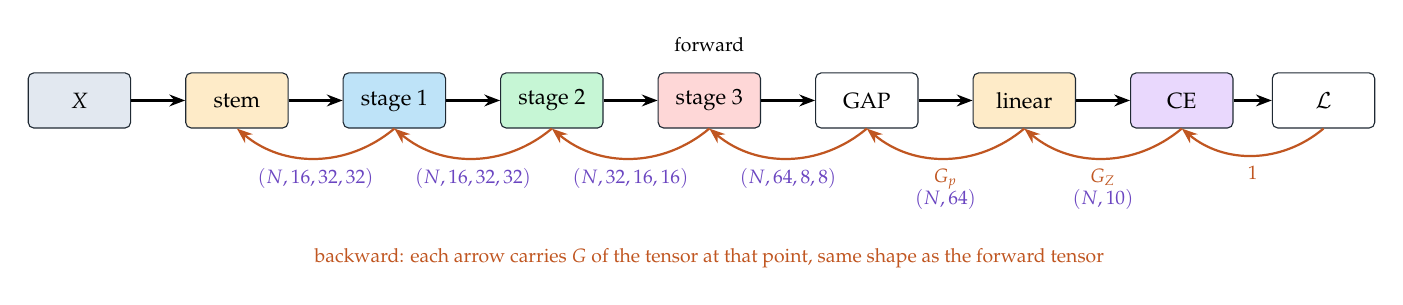
\begin{tikzpicture}[
  n/.style={draw=ink,rounded corners=2pt,fill=#1,font=\footnotesize,minimum height=0.7cm,minimum width=1.3cm,align=center,inner sep=3pt},
  n/.default=white, ar/.style={-{Stealth[length=2mm]},thick}, br/.style={-{Stealth[length=2mm]},thick,warn}]
  \foreach \nm/\lab/\col/\xx in {x/{$X$}/cIn/0,st/stem/cK/2,s1/{stage 1}/c16/4,s2/{stage 2}/c32/6,s3/{stage 3}/c64/8,gap/GAP/white/10,lin/linear/cK/12,ce/CE/cG/14,L/{$\mathcal L$}/white/15.8}
    \node[n=\col] (\nm) at (\xx,0) {\lab};
  \foreach \a/\b in {x/st,st/s1,s1/s2,s2/s3,s3/gap,gap/lin,lin/ce,ce/L} \draw[ar] (\a) -- (\b);
  \node[font=\scriptsize,above] at (8,0.5) {forward};
  \foreach \a/\b/\t in {L/ce/{$1$},ce/lin/{$G_Z$\\\shp{N,10}},lin/gap/{$G_p$\\\shp{N,64}},gap/s3/{\shp{N,64,8,8}},s3/s2/{\shp{N,32,16,16}},s2/s1/{\shp{N,16,32,32}},s1/st/{\shp{N,16,32,32}}}
    \draw[br] (\a.south) to[bend left=40] node[below,font=\scriptsize,align=center,warn]{\t} (\b.south);
  \node[font=\scriptsize,warn] at (8,-2.0) {backward: each arrow carries $G$ of the tensor at that point, same shape as the forward tensor};
\end{tikzpicture}}
\end{center}

\subsection{Cross-entropy with softmax: the gradient on the logits}
\label{sec:cegrad}

\begin{idea}[derivation]
For one example, $\ell = \operatorname{logsumexp}(z) - z_y$. Since $\partial\operatorname{logsumexp}(z)/\partial z_k = e^{z_k}/\sum_je^{z_j} = s_k$,
\[
  \dd{\ell}{z_k} = s_k - \mathbb 1[k=y].
\]
With the batch mean $\mathcal L=\frac1N\sum_n\ell_n$:
\[
  \boxed{\,G_Z = \tfrac1N\,(S - Y_\text{onehot})\,}\qquad S,\;Y_\text{onehot},\;G_Z\in\R^{N\times10}.
\]
The gradient on the logits is ``predicted probability minus target'', divided by the batch size. Each row sums to zero. The correct class is pushed up by $1-s_y$, and every wrong class is pushed down by its own probability.
\end{idea}

\begin{repo}[on \texttt{test0.png}, $N=1$]
$G_z = s - e_3 = (6.7{\times}10^{-13},\,3.6{\times}10^{-11},\,6.0{\times}10^{-11},\,\mathbf{-1.58{\times}10^{-7}},\,\dots,\,1.55{\times}10^{-7}\,(\text{dog}),\,\dots)$. Almost no gradient: a confidently correct example teaches the model nothing more. During training the batch average is dominated by the hard and misclassified examples.
\end{repo}

\subsection{Linear layer}

\begin{idea}[three matrix products, each shape-checked]
Forward $Z = PW\T + \mathbf 1 b\T$ with $P\in\R^{N\times64}$, $W\in\R^{10\times64}$. Then
\begin{align*}
  G_W &= G_Z\T\,P &&(10\times N)(N\times64) = (10\times64) \;\checkmark\;\text{same as }W\\
  G_b &= G_Z\T\,\mathbf 1_N = \textstyle\sum_n G_Z[n,:] &&(10)\\
  G_P &= G_Z\,W &&(N\times10)(10\times64) = (N\times64)\;\checkmark\;\text{same as }P
\end{align*}
The mnemonic: \emph{the gradient of a matrix product with respect to one factor is the upstream gradient multiplied by the transpose of the other factor, placed on whichever side makes the shapes fit}. The sum over the batch in $G_W$ and $G_b$ is the inner dimension $N$ disappearing: the parameter gradient accumulates over all examples.
\end{idea}

\begin{center}
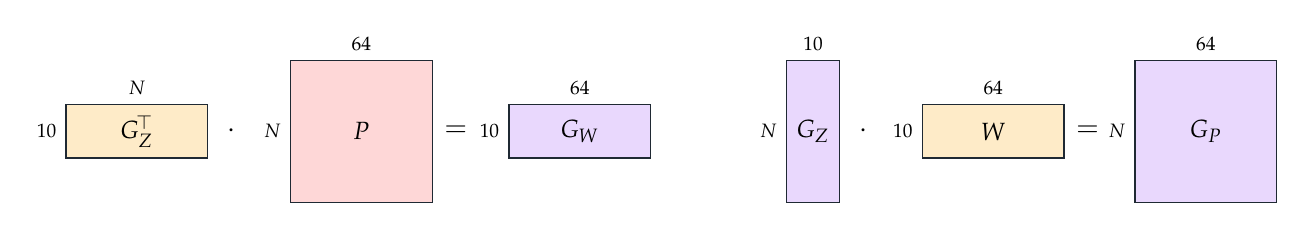
\begin{tikzpicture}[scale=0.75]
  \matr{0.5}{0.75}{2.4}{0.9}{cK}{$G_Z\T$}{$10$}{$N$}
  \node at (3.3,1.2) {$\cdot$};
  \matr{4.3}{0}{2.4}{2.4}{c64}{$P$}{$N$}{$64$}
  \node at (7.1,1.2) {$=$};
  \matr{8.0}{0.75}{2.4}{0.9}{cG}{$G_W$}{$10$}{$64$}
  \begin{scope}[shift={(12.2,0)}]
  \matr{0.5}{0}{0.9}{2.4}{cG}{$G_Z$}{$N$}{$10$}
  \node at (1.8,1.2) {$\cdot$};
  \matr{2.8}{0.75}{2.4}{0.9}{cK}{$W$}{$10$}{$64$}
  \node at (5.6,1.2) {$=$};
  \matr{6.4}{0}{2.4}{2.4}{cG}{$G_P$}{$N$}{$64$}
  \end{scope}
\end{tikzpicture}
\end{center}

\subsection{Flatten and global average pooling}

\begin{idea}
Flatten backward is a reshape: $G\in\R^{N\times64}\to\R^{N\times64\times1\times1}$. GAP averaged 64 positions with weight $1/64$ each, so each position receives $1/64$ of the gradient:
\[
  G_A[n,c,h,w] = \tfrac{1}{64}\,G_p[n,c], \qquad \shp{N,64}\;\xrightarrow{\text{broadcast}}\;\shp{N,64,8,8}.
\]
Every location of a stage-3 feature map gets the same gradient. GAP does not care where the evidence was.
\end{idea}

\subsection{ReLU}

\begin{idea}
$G_z = G_y\odot\mathbb 1[z>0]$. Gradient flows unchanged through active units and is blocked at inactive ones. Autograd needs to remember only the output (or the mask), not the input.
\end{idea}

\subsection{The residual addition and the option-A shortcut}
\label{sec:shortcut-back}

\begin{idea}[an addition copies the gradient to both inputs]
For $u=\mathcal F(x)+s(x)$: $\partial u/\partial\mathcal F = I$ and $\partial u/\partial s = I$, so $G_\mathcal F = G_u$ and $G_s = G_u$. Then
\[
  G_x = \underbrace{\big(\text{branch backward of }G_u\big)}_{\text{through 2 convs, 2 BNs, 1 ReLU}} \;+\; \underbrace{\big(\text{shortcut backward of }G_u\big)}_{\text{identity: just }G_u} .
\]
This is the ``gradient highway'' of \cref{sec:whyres}, now concretely: the shortcut contributes $G_u$ itself to $G_x$, untouched by any weight.
\end{idea}

\begin{repo}[backward of \texttt{F.pad(x[:,:,::2,::2], (0,0,0,0,8,8))}]
Run the two forward steps backwards. With $G_s\in\R^{N\times32\times16\times16}$:
\begin{enumerate}[nosep]
  \item \textbf{Pad backward = slice.} The zero channels did not depend on $x$, so their gradient is discarded: $G_\text{sub} = G_s[:,\,8{:}24,\,:,\,:]\in\R^{N\times16\times16\times16}$.
  \item \textbf{Strided slice backward = scatter.} Allocate $G\in\R^{N\times16\times32\times32}$ filled with zeros and write $G[:,:,::2,::2] = G_\text{sub}$.
\end{enumerate}
So the shortcut sends gradient only to the even-row, even-column positions of the input (a quarter of them) and only from the middle 16 output channels. The other three quarters of the positions get gradient only through the residual branch's stride-2 convolution.
\end{repo}

\begin{center}
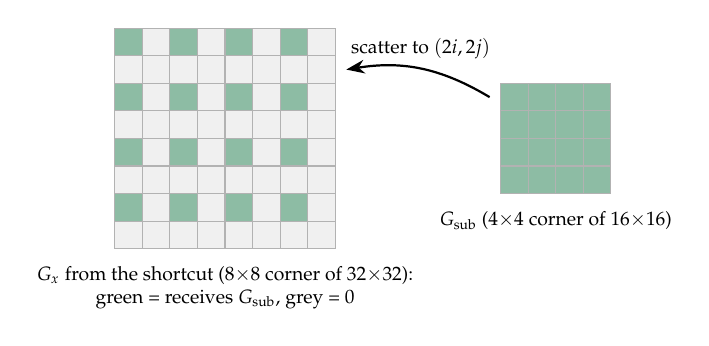
\begin{tikzpicture}[scale=0.35]
  \foreach \i in {0,...,7} \foreach \j in {0,...,7} {
    \pgfmathtruncatemacro{\ev}{(mod(\i,2)==0 && mod(\j,2)==0) ? 1 : 0}
    \ifnum\ev=1 \fill[repo!55] (\j,-\i) rectangle ++(1,1); \else \fill[black!6] (\j,-\i) rectangle ++(1,1); \fi
    \draw[black!30] (\j,-\i) rectangle ++(1,1);
  }
  \node[font=\scriptsize,align=center,below] at (4,-7.3) {$G_x$ from the shortcut ($8{\times}8$ corner of $32{\times}32$):\\green = receives $G_\text{sub}$, grey = 0};
  \foreach \i in {0,...,3} \foreach \j in {0,...,3} {\fill[repo!55] (14+\j,-\i-2) rectangle ++(1,1); \draw[black!30] (14+\j,-\i-2) rectangle ++(1,1);}
  \node[font=\scriptsize,below,align=center] at (16,-5.3) {$G_\text{sub}$ ($4{\times}4$ corner of $16{\times}16$)};
  \draw[-{Stealth},thick] (13.6,-1.5) to[bend right=20] node[above,font=\scriptsize]{scatter to $(2i,2j)$} (8.4,-0.5);
\end{tikzpicture}
\end{center}

\subsection{Batch normalisation (train mode)}
\label{sec:bnback}

\begin{idea}[derivation in four lines]
Fix a channel and drop the index $c$. Write $m=NHW$, $\hat a_k=(a_k-\mu)/\sigma_\varepsilon$ with $\sigma_\varepsilon=\sqrt{\sigma^2+\varepsilon}$, and $y_k=\gamma\hat a_k+\beta$, for $k$ running over the $m$ positions. The parameter gradients are immediate:
\[
  G_\gamma = \sum_{k=1}^m G_{y_k}\,\hat a_k, \qquad G_\beta = \sum_{k=1}^m G_{y_k}.
\]
For the input, $\mu$ and $\sigma^2$ depend on \emph{every} $a_k$ in the channel, so each $a_k$ affects every $y_j$. Using $\partial\mu/\partial a_k = 1/m$ and $\partial\sigma^2/\partial a_k = 2(a_k-\mu)/m$ and collecting terms:
\[
  \boxed{\;G_{a_k} = \frac{\gamma}{m\,\sigma_\varepsilon}\Big(m\,G_{y_k} \;-\; \sum_{j}G_{y_j} \;-\; \hat a_k\sum_j G_{y_j}\hat a_j\Big)\;}
\]
The upstream gradient is centred (its mean over the channel is removed), and its component along $\hat a$ is removed, then rescaled by $\gamma/\sigma_\varepsilon$. Hence a BN layer cannot pass back a gradient that would merely shift or rescale its input channel. Those directions are taken over by $\beta$ and $\gamma$.
\end{idea}

\begin{shapebox}[BN backward]
$G_y, G_a\in\R^{N\times C\times H\times W}$. The sums run over axes $(0,2,3)$ and give shape \shp{C}, broadcast back as \shp{1,C,1,1}. $G_\gamma,G_\beta\in\R^{C}$. In eval mode BN is the fixed affine $y=a_cx+b_c$, so its backward would be simply $G_x=a_c\,G_y$. Training never back-propagates in eval mode, though.
\end{shapebox}

\subsection{Convolution}
\label{sec:convback}

\begin{idea}[two gradients, both are convolutions again]
From $Y[n,o,i,j]=\sum_{c,u,v}\mathcal W[o,c,u,v]\,\tilde X[n,c,Si{+}u,Sj{+}v]$:

\textbf{Weight gradient}: correlate the (padded) input with the output gradient, summing over the batch:
\[
  G_\mathcal W[o,c,u,v] = \sum_{n}\sum_{i,j} G_Y[n,o,i,j]\;\tilde X[n,c,\,Si+u,\,Sj+v].
\]
\textbf{Input gradient}: every input pixel collects gradient from every output window that contained it:
\[
  G_{\tilde X}[n,c,a,b] = \sum_{o}\sum_{\substack{i,j,u,v:\\ Si+u=a,\;Sj+v=b}} G_Y[n,o,i,j]\;\mathcal W[o,c,u,v],
\]
and $G_X$ is $G_{\tilde X}$ with the $P$-pixel border cropped off. This is a ``full'' convolution of $G_Y$ (with zeros inserted between entries when $S=2$) with the $180^\circ$-rotated kernel, with the in/out channel roles swapped. It is exactly what \code{conv\_transpose2d} computes.
\end{idea}

\begin{idea}[the same thing in im2col form: two more matrix products]
With $Y_\text{mat}=W_\text{mat}X_\text{col}$ (\cref{sec:im2col}) and $G_{Y_\text{mat}}\in\R^{C_\text{out}\times H_\text{out}W_\text{out}}$:
\begin{align*}
  G_{W_\text{mat}} &= \sum_n G_{Y_\text{mat}}^{(n)}\,X_\text{col}^{(n)\top}
    && (C_\text{out}\times HW)(HW\times C_\text{in}K^2) = (C_\text{out}\times C_\text{in}K^2)\;\checkmark\\
  G_{X_\text{col}} &= W_\text{mat}\T\,G_{Y_\text{mat}}
    && (C_\text{in}K^2\times C_\text{out})(C_\text{out}\times HW) = (C_\text{in}K^2\times HW)\;\checkmark
\end{align*}
then \emph{col2im}: scatter-add each column of $G_{X_\text{col}}$ back into the $C_\text{in}\times K\times K$ window it came from. Overlapping windows add up, which is where the ``sum over windows containing the pixel'' comes from. These are exactly the linear-layer rules, with $X_\text{col}$ playing $P$ and $W_\text{mat}$ playing $W$.
\end{idea}

\begin{center}
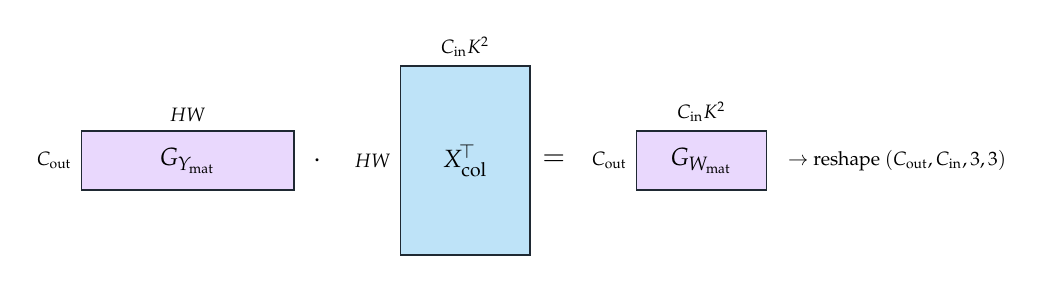
\begin{tikzpicture}[scale=0.75]
  \matr{0.8}{0.6}{3.6}{1.0}{cG}{$G_{Y_\text{mat}}$}{$C_\text{out}$}{$HW$}
  \node at (4.8,1.1) {$\cdot$};
  \matr{6.2}{-0.5}{2.2}{3.2}{c16}{$X_\text{col}\T$}{$HW$}{$C_\text{in}K^2$}
  \node at (8.8,1.1) {$=$};
  \matr{10.2}{0.6}{2.2}{1.0}{cG}{$G_{W_\text{mat}}$}{$C_\text{out}$}{$C_\text{in}K^2$}
  \node[font=\scriptsize,right] at (12.6,1.1) {$\to$ reshape $(C_\text{out},C_\text{in},3,3)$};
\end{tikzpicture}
\end{center}

\begin{shapebox}[conv gradients in this network]
\begin{center}
\small
\begin{tabular}{@{}lllll@{}}
\toprule
conv & $X$ & $Y$ & $G_\mathcal W$ (= shape of $\mathcal W$) & $G_X$\\
\midrule
stem & \shp{N,3,32,32} & \shp{N,16,32,32} & \shp{16,3,3,3} & (not needed)\\
stage-1 conv & \shp{N,16,32,32} & \shp{N,16,32,32} & \shp{16,16,3,3} & \shp{N,16,32,32}\\
stage-2 first ($S{=}2$) & \shp{N,16,32,32} & \shp{N,32,16,16} & \shp{32,16,3,3} & \shp{N,16,32,32}\\
stage-3 first ($S{=}2$) & \shp{N,32,16,16} & \shp{N,64,8,8} & \shp{64,32,3,3} & \shp{N,32,16,16}\\
stage-3 conv & \shp{N,64,8,8} & \shp{N,64,8,8} & \shp{64,64,3,3} & \shp{N,64,8,8}\\
\bottomrule
\end{tabular}
\end{center}
The input image needs no gradient (\code{requires\_grad=False}), so autograd skips $G_X$ for the stem. A stride-2 conv's $G_X$ is back at the \emph{larger} resolution: back-propagation undoes the downsampling.
\end{shapebox}

\subsection{One whole block backwards}

\begin{repo}[gradient flow through \texttt{BasicBlock.forward}, reversed]
Given $G_y$ (shape of the block output):
\begin{align*}
  G_u &= G_y\odot\mathbb 1[u>0] && u=\mathcal F(x)+s(x)\\
  G_{b_2} &= G_u && \text{(add: copy to branch)}\\
  G_{a_2},\,G_{\gamma_2},\,G_{\beta_2} &= \text{BN-backward}(G_{b_2}) && \text{\cref{sec:bnback}}\\
  G_{r_1},\,G_{\mathcal W_2} &= \text{conv-backward}(G_{a_2}) && \text{\cref{sec:convback}}\\
  G_{b_1} &= G_{r_1}\odot\mathbb 1[b_1>0]\\
  G_{a_1},\,G_{\gamma_1},\,G_{\beta_1} &= \text{BN-backward}(G_{b_1})\\
  G_x^{\text{branch}},\,G_{\mathcal W_1} &= \text{conv-backward}(G_{a_1}) && \text{(stride $S$)}\\
  G_x &= G_x^{\text{branch}} + \begin{cases}G_u & \text{identity shortcut}\\ \text{scatter}\big(G_u[:,\,p{:}p{+}C_\text{in}]\big) & \text{option A}\\ 0 & \text{plain}\end{cases}
\end{align*}
where $p=(C_\text{out}-C_\text{in})/2$ is the number of padded channels on each side (8 or 16).
\code{loss.backward()} does all of this automatically, for all 9 blocks, the stem and the head. Afterwards every parameter's \code{.grad} holds $G_\theta$ with \code{.grad.shape == param.shape}: this was checked for every parameter, e.g.\ \code{stage2.0.first\_conv.weight} \shp{32,16,3,3}, \code{linear.weight} \shp{10,64}, \code{bn1.weight} \shp{16}.
\end{repo}

\begin{warn}[what \texttt{train\_step} does around backward]
\begin{lstlisting}[firstnumber=4]
def train_step(model,x,y,optimizer,loss_fn):
    optimizer.zero_grad()
    logits = model(x)
    loss = loss_fn(logits,y)
    loss.backward()
    optimizer.step()
    return logits.detach(), loss.item()
\end{lstlisting}
PyTorch \emph{accumulates} into \code{.grad}, so \code{zero\_grad()} must come first. In PyTorch 2.x it sets \code{.grad} to \code{None} (the default \code{set\_to\_none=True}) rather than filling with zeros. The returned logits are those of the forward pass \emph{before} the update, detached from the graph, and they are what the epoch's training accuracy is computed from (\cref{sec:loop}). \code{loss.item()} copies the scalar to the CPU, which synchronises with the GPU once per step.
\end{warn}

\section{Optimisation: SGD, the schedule and the training loop}
\label{sec:optim}

\subsection{The optimiser}
\label{sec:sgd}

\begin{repo}[\texttt{scripts/train\_resnet.py}]
\begin{lstlisting}[firstnumber=56]
optim = torch.optim.SGD(params=model.parameters(),lr=0.1,momentum=0.9,weight_decay=1e-4)
loss_fct = nn.CrossEntropyLoss()
\end{lstlisting}
One parameter group containing all 269{,}722 parameters, with \code{dampening=0} and \code{nesterov=False} (defaults).
\end{repo}

\begin{idea}[the exact update PyTorch performs]
At step $t$, for every parameter tensor $\theta$ (all shapes are the parameter's own shape):
\begin{align*}
  g_t &= \nabla_\theta\mathcal L(\theta_t) + \lambda\,\theta_t && \text{weight decay folded into the gradient}\\
  v_t &= \begin{cases} g_t & t=1\\ \mu\,v_{t-1} + g_t & t>1\end{cases} && \text{momentum buffer (velocity)}\\
  \theta_{t+1} &= \theta_t - \eta_t\,v_t && \text{step}
\end{align*}
with $\mu=0.9$, $\lambda=10^{-4}$ and $\eta_t$ from the schedule. The momentum buffer is initialised to the first gradient, not to zero. Unrolled, $v_t=\sum_{k\le t}\mu^{t-k}g_k$ is an exponentially weighted sum of past gradients with an effective memory of $1/(1-\mu)=10$ steps. Under a constant gradient $g$, $v\to g/(1-\mu)=10g$, so \textbf{the effective step size is $10\eta$}: $1.0$, then $0.1$, then $0.01$.
\end{idea}

\begin{warn}[two momentum conventions]
Some papers and frameworks (e.g.\ Sutskever et al.\ 2013, Caffe) put the learning rate \emph{inside} the velocity, $v_t=\mu v_{t-1}-\eta_t g_t$, $\theta_{t+1}=\theta_t+v_t$. With a constant $\eta$ the two are identical ($v^\text{Caffe}=-\eta\,v^\text{PyTorch}$). They differ only at a learning-rate drop. In PyTorch the stored velocity is unchanged and gets multiplied by the new, smaller $\eta$, so the step shrinks $10\times$ immediately. In the other form the old velocity still carries the old $\eta$ and fades over $\sim$20 steps. Over 16{,}000-iteration phases the difference is negligible, but it is worth knowing when reading other code.
\end{warn}

\begin{repo}[one step verified]
Three steps of the update above, written out by hand, reproduce \code{torch.optim.SGD(lr=0.1, momentum=0.9, weight\_decay=1e-4)} to within $4\times10^{-6}$ (\code{float32}). The optimiser state is one momentum buffer per parameter tensor, with the same shape, i.e.\ another 269{,}722 numbers. That is why the training checkpoints (2.2\,MB) are twice the size of the exported serving weights (1.1\,MB).
\end{repo}

\subsection{Weight decay}
\label{sec:wd}

\begin{idea}[L2 regularisation, and what it does with BN]
Adding $\lambda\theta$ to the gradient is gradient descent on
\[
  \mathcal L(\theta) + \tfrac{\lambda}{2}\|\theta\|_2^2 ,
\]
so with plain SGD, ``weight decay'' and ``L2 penalty'' are the same thing. (They differ only for adaptive optimisers like Adam, hence AdamW.) Each step shrinks every weight by the factor $(1-\eta\lambda)$ before the gradient step: $1-10^{-5}$ per step at $\eta=0.1$.

In a network where every conv is followed by BN, the conv's output is invariant to rescaling its weights ($\BN(\alpha\,\mathcal W*x)=\BN(\mathcal W*x)$ for $\alpha>0$). The penalty therefore does not change the function, but it keeps $\|\mathcal W\|$ small, and a small $\|\mathcal W\|$ makes the same $\eta$ a \emph{larger relative} step. Weight decay on BN-ed convs acts largely as a control on the effective learning rate.
\end{idea}

\begin{repo}[applied to every parameter]
Because \code{model.parameters()} goes into a single group, decay applies to conv weights, BN $\gamma$ \emph{and} $\beta$, and the linear weight and bias alike. The paper does not say whether BN parameters were excluded; many reimplementations decay everything, as here. Measured on the final model: $\|\theta\|_2^2 = 3218.6$, so the penalty term is $\tfrac{\lambda}{2}\|\theta\|^2 = 0.161$. At the end of training the data loss is $0.024$, so \textbf{the regulariser is about $6.6\times$ the data term} of the objective SGD is actually minimising. Its visible fingerprint is stem channel 0 (\cref{sec:forward}): its filter norm decayed to $0.047$ and its $\gamma$ to $0.011$, a channel the data did not defend.
\end{repo}

\subsection{The learning-rate schedule}
\label{sec:schedule}

\begin{lstlisting}[firstnumber=60]
def lr_at(iteration):
    if iteration < 32000:
        return 0.1
    elif iteration < 48000:
        return 0.01
    else:
        return 0.001
def set_lr(optimizer,lr):
    for p in optimizer.param_groups:
        p["lr"] = lr
\end{lstlisting}

\begin{idea}[step decay, counted in iterations]
$\eta_t = 0.1\cdot 10^{-\,[t\ge32000]-[t\ge48000]}$, where $t$ is the number of optimiser steps already taken. The paper specifies the schedule in iterations (``divide it by 10 at 32k and 48k iterations, and terminate training at 64k iterations''), independent of the dataset size, which is why the repo counts iterations, not epochs.
\end{idea}

\begin{center}
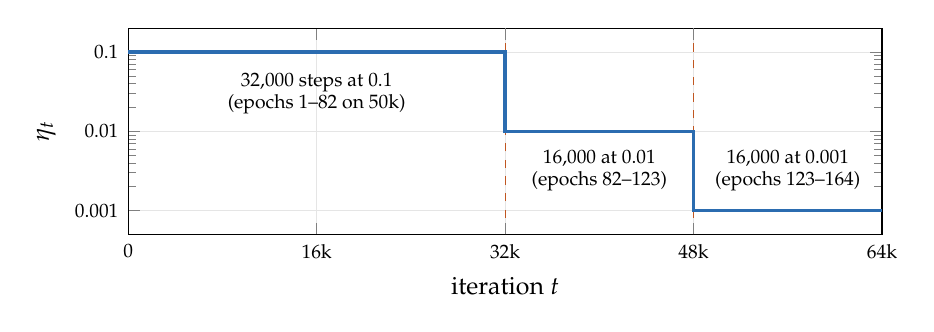
\begin{tikzpicture}
\begin{axis}[width=0.92\linewidth,height=4.2cm,ymode=log,xmin=0,xmax=64000,ymin=0.0005,ymax=0.2,
  xlabel={iteration $t$},ylabel={$\eta_t$},xtick={0,16000,32000,48000,64000},
  xticklabels={0,16k,32k,48k,64k},ytick={0.001,0.01,0.1},yticklabels={0.001,0.01,0.1},
  grid=major,grid style={black!10},tick label style={font=\scriptsize},label style={font=\small},scaled x ticks=false,
  extra x ticks={32000,48000},extra x tick labels={},extra x tick style={grid style={warn,dashed}}]
  \addplot[const plot,very thick,idea] coordinates {(0,0.1) (32000,0.01) (48000,0.001) (64000,0.001)};
  \node[font=\scriptsize,align=center] at (axis cs:16000,0.03) {32{,}000 steps at 0.1\\(epochs 1--82 on 50k)};
  \node[font=\scriptsize,align=center] at (axis cs:40000,0.0032) {16{,}000 at 0.01\\(epochs 82--123)};
  \node[font=\scriptsize,align=center] at (axis cs:56000,0.0032) {16{,}000 at 0.001\\(epochs 123--164)};
\end{axis}
\end{tikzpicture}
\end{center}

\begin{repo}[iterations $\leftrightarrow$ epochs]
\begin{center}
\small
\begin{tabular}{@{}lrrrrr@{}}
\toprule
run & iters/epoch & 1st drop (32k) & 2nd drop (48k) & end (64k) & last epoch\\
\midrule
final (50k) & 391 & during epoch 82 & during epoch 123 & epoch 164 & 267 iterations\\
development (45k) & 352 & during epoch 91 & during epoch 137 & epoch 182 & 288 iterations\\
\bottomrule
\end{tabular}
\end{center}
$64{,}000\times128 = 8{,}192{,}000$ examples are seen, $163.84$ passes over 50k (counting the short last batch of each epoch as a full step, which is what the loop does). $163\cdot391=63{,}733$ iterations finish 163 epochs, and epoch 164 stops after $267$ more, exactly as in \file{artifacts/logs/final\_res20.csv} (last row: epoch 164, iteration 64{,}000). The learning rate is set \emph{before} every step from the current count, so step 0 through step 31{,}999 use 0.1 (\file{check\_schedule.py} tests the boundaries 31999/32000 and 47999/48000). Every BN layer's \code{num\_batches\_tracked} in the checkpoint reads exactly \textbf{64{,}000}: one train-mode forward per optimiser step, with no extra ones.
\end{repo}

\subsection{The training loop}
\label{sec:loop}

\begin{lstlisting}[firstnumber=33]
def train_one_epoch(model,loader,optimizer,loss_fn,device,iteration,max_iterations):
    model.train()
    num_exmpl  = 0
    correct_pred = 0
    loss_cum = 0
    iterer = iteration
    for image,label in loader:
        image = image.to(device)
        label = label.to(device)
        if iterer >= max_iterations:
             break
        set_lr(optimizer, lr_at(iterer))
        logits,loss = train_step(model=model,x=image,y=label,optimizer=optimizer,loss_fn=loss_fn)
        compare = (torch.argmax(logits,dim=1) == label)
        compare = compare.sum().item()
        correct_pred+= compare
        iterer+=1
        num_exmpl += logits.shape[0]
        loss_cum+=loss*logits.shape[0]
    loss_cum /= num_exmpl
    correct_pred /= num_exmpl
    return loss_cum,correct_pred,iterer
\end{lstlisting}

\begin{center}
\resizebox{\linewidth}{!}{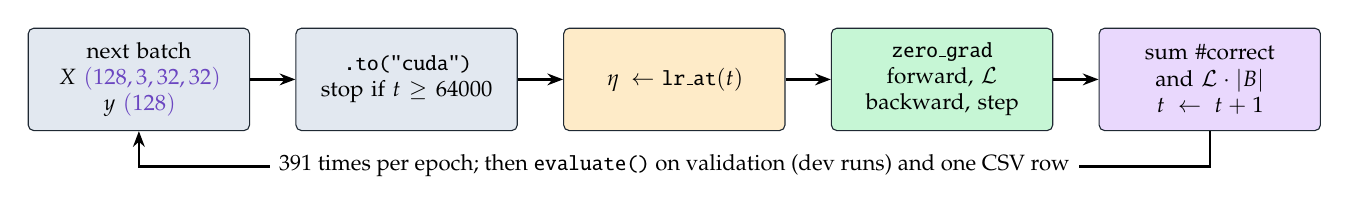
\begin{tikzpicture}[
  n/.style={draw=ink,rounded corners=2pt,fill=#1,font=\footnotesize,minimum height=1.3cm,align=center,inner sep=3pt,text width=2.6cm},
  n/.default=white, ar/.style={-{Stealth[length=2mm]},thick}]
  \node[n=cIn] (a) at (0,0) {next batch\\$X$ \shp{128,3,32,32}\\$y$ \shp{128}};
  \node[n=cIn] (b) at (3.4,0) {\code{.to("cuda")}\\stop if $t\ge64000$};
  \node[n=cK] (c) at (6.8,0) {$\eta\leftarrow$ \code{lr\_at}$(t)$};
  \node[n=c32] (d) at (10.2,0) {\code{zero\_grad}\\forward, $\mathcal L$\\backward, step};
  \node[n=cG] (e) at (13.6,0) {sum \#correct\\and $\mathcal L\cdot|B|$\\$t\leftarrow t+1$};
  \foreach \p/\q in {a/b,b/c,c/d,d/e} \draw[ar] (\p) -- (\q);
  \draw[ar] (e.south) -- ++(0,-0.45) -| (a.south);
  \node[font=\footnotesize,fill=white] at (6.8,-1.1) {391 times per epoch; then \code{evaluate()} on validation (dev runs) and one CSV row};
\end{tikzpicture}}
\end{center}

\begin{repo}[what the logged training metrics mean]
\begin{itemize}[nosep]
  \item \textbf{train\_loss}: $\sum_\text{batches}\mathcal L_B\,|B|\big/\sum|B|$, the exact per-example average over the epoch, correct also for the short last batch.
  \item \textbf{train\_acc}: computed from the logits of each step's forward pass, i.e.\ on \emph{augmented} images, with \emph{train-mode} BN, and \emph{before} that step's update. The model changes during the epoch, so this is a running average, not the accuracy of the end-of-epoch model. The README's ``train error'' column (e.g.\ 0.52\% for ResNet-20) is this quantity at the last epoch.
  \item \textbf{val\_loss / val\_acc}: from \code{evaluate()} after the epoch, in eval mode, on un-augmented validation images. Empty in the \code{--full} run, which has no validation set.
  \item \textbf{lr}: read from \code{optim.param\_groups[0]["lr"]} after the epoch, i.e.\ the rate of its last step.
\end{itemize}
\end{repo}

\begin{center}
\begin{tikzpicture}
\begin{axis}[width=0.95\linewidth,height=6.2cm,xmin=0,xmax=64000,ymin=0,ymax=30,
  xlabel={iteration},ylabel={error (\%)},xtick={0,16000,32000,48000,64000},xticklabels={0,16k,32k,48k,64k},scaled x ticks=false,
  grid=major,grid style={black!10},tick label style={font=\scriptsize},label style={font=\small},
  legend style={font=\scriptsize,at={(0.98,0.97)},anchor=north east,draw=black!20},legend cell align=left]
  \addplot[idea,thick] table[col sep=comma,x=iteration,y expr={100*(1-\thisrow{train_acc})}] {logs/final_res20.csv};
  \addlegendentry{final run (50k): train error (augmented, train mode)}
  \addplot[warn,thick] table[col sep=comma,x=iteration,y expr={100*(1-\thisrow{val_acc})}] {logs/dev_res20.csv};
  \addlegendentry{development run (45k): validation error}
  \addplot[warn!50,thin] table[col sep=comma,x=iteration,y expr={100*(1-\thisrow{train_acc})}] {logs/dev_res20.csv};
  \addlegendentry{development run (45k): train error}
  \draw[black!50,dashed] (axis cs:32000,0) -- (axis cs:32000,30);
  \draw[black!50,dashed] (axis cs:48000,0) -- (axis cs:48000,30);
\end{axis}
\end{tikzpicture}
\end{center}

The two learning-rate drops are the most visible events in training. At the first drop, the development run's validation error falls from $17.6\%$ (epoch 90, $\eta=0.1$, noisy) to $9.8\%$ one epoch later and $8.8\%$ the epoch after. The second drop gives a smaller, final improvement. At $\eta=0.1$ the validation curve is noisy because the effective step ($10\eta=1$) keeps the weights bouncing around a wide region. Smaller steps let SGD settle into it. The final run takes 2{,}182\,s ($\approx36$ minutes) on an RTX 3050, about 13\,s per epoch.

\subsection{Seeds, checkpoints and the run script}

\begin{repo}[sources of randomness, and what controls each]
\begin{center}
\small
\begin{tabularx}{\linewidth}{@{}>{\raggedright\arraybackslash}p{3.2cm}>{\raggedright\arraybackslash}X>{\raggedright\arraybackslash}X@{}}
\toprule
randomness & generator & seeded by\\
\midrule
weight initialisation & PyTorch global RNG & \code{torch.manual\_seed(args.seed)}, before the model is built\\
batch order & \code{torch.Generator g} passed to the loader & \code{g.manual\_seed(args.seed)}\\
crop offsets and flips & \code{np.random.default\_rng} in the dataset & \code{seed=args.seed}\\
train/val split & local \code{torch.Generator} & literal 0\\
GPU kernels & cuDNN algorithm choice & \emph{not controlled}\\
\bottomrule
\end{tabularx}
\end{center}
All reported runs use seed 0. Without \code{torch.backends.cudnn.deterministic=True}, re-running is reproducible up to floating-point noise, not bit-for-bit.
\end{repo}

\begin{repo}[checkpoints]
\code{save\_checkpoint} writes one dictionary,
\begin{center}\code{\{"model": state\_dict, "optimizer": state\_dict, "iteration": t, "seed": s\}},\end{center}
\emph{once}, at the end of training. Nothing is saved per epoch, so an interrupted run restarts from scratch. \code{load\_checkpoint} restores the model, restores the optimiser only if one is passed (the service passes \code{None}), and returns \code{(iteration, seed)}. \file{scripts/export\_model.py} re-saves the final weights without the optimiser state as \file{model/resnet20.pt} (1{,}121{,}617 bytes, 116 \code{state\_dict} entries) and copies the 50k mean next to it. Those two files are all the service needs.
\end{repo}

\begin{repo}[command line]
\code{python -m scripts.train\_resnet --name final\_res20 --full} for the headline model; \code{--n 9} for ResNet-56; \code{--plain} for the plain networks; \code{--max-iters} to shorten a run. The device is hard-coded to \code{"cuda"}.
\end{repo}

\subsection{Sanity checks that were run before the full training}

\begin{repo}[\texttt{scripts/}]
\begin{itemize}[nosep]
  \item \file{overfit\_batch.py}: 200 steps on one fixed batch of 128. A correct model, loss and optimiser must drive this to $\approx100\%$ training accuracy. If they cannot, something is broken before any hyperparameter matters. The first loss should be $\approx\ln10=2.30$. One random batch at initialisation gives $2.42$, slightly above because of the randomly initialised linear layer.
  \item \file{check\_model.py}: parameter counts for $n=3$ and $9$, residual and plain; output shape \shp{128,10}; initial weight standard deviations.
  \item \file{check\_schedule.py}: \code{lr\_at} on both sides of each boundary.
  \item \file{check\_checkpoint.py}: train 20 steps, save, load into a fresh model, and verify identical \code{state\_dict}s and identical validation metrics.
  \item \file{check\_eval.py}: train-mode forward passes followed by \code{evaluate()}, which must switch BN to eval mode.
  \item \file{check\_loader.py}, \file{check\_split.py}, \file{check\_mean.py}, \file{check\_augment.py}: data pipeline determinism and shapes, with the augmentation grid saved to \file{artifacts/aug\_grid.png}.
\end{itemize}
\end{repo}

\section{Evaluation: eval mode, metrics and results}
\label{sec:eval}

\subsection{What changes in eval mode}
\label{sec:evalbn}

\begin{idea}[BN collapses to a per-channel affine map]
With the running statistics frozen, BN no longer depends on the batch:
\[
  y = \gamma_c\frac{x-r_{\mu,c}}{\sqrt{r_{\sigma^2,c}+\varepsilon}}+\beta_c
    = a_c\,x + b_c,\qquad a_c=\frac{\gamma_c}{\sqrt{r_{\sigma^2,c}+\varepsilon}},\quad b_c=\beta_c-a_c\,r_{\mu,c}.
\]
Because the preceding conv is linear, the BN could even be \emph{folded} into it: $\mathcal W'[o]=a_o\mathcal W[o]$, bias $b_o$. The repo does not fold. Eval-mode predictions are deterministic and independent of what else is in the batch, so a batch of 1 in the service behaves exactly like a batch of 128 in the evaluation.
\end{idea}

\begin{repo}[\texttt{evaluate()} and \texttt{predict()}]
Both call \code{model.eval()} and run inside \code{torch.no\_grad()}, so no graph is stored and the BN buffers are not touched. \code{evaluate} returns the example-weighted mean loss and the accuracy. \code{predict} returns \code{softmax(logits, dim=1)} for every test image as a NumPy array \shp{10000,10} plus the labels \shp{10000}. \file{eval\_test.py} saves both to \file{artifacts/preds/<name>.npz}, and every metric below is computed from that file. ResNet has no dropout, so BN is the only layer whose behaviour differs between the two modes.
\end{repo}

\subsection{Confusion matrix}

\begin{idea}
$C\in\mathbb N^{10\times10}$ with $C[t,p]=\#\{\text{test images of true class }t\text{ predicted as }p\}$. Rows sum to the class sizes (1{,}000 each), and the trace counts the correct predictions. Accuracy $=\operatorname{tr}(C)/\sum C$.
\end{idea}

\begin{repo}[the final ResNet-20 on the 10{,}000 test images]
\begin{center}
\scriptsize
\setlength{\tabcolsep}{4.5pt}
\begin{tabular}{@{}r|cccccccccc|r@{}}
true $\backslash$ pred & plane & car & bird & \textbf{cat} & deer & \textbf{dog} & frog & horse & ship & truck & recall\\
\midrule
plane & \textbf{923} & 4 & 23 & 10 & 5 & 0 & 3 & 1 & 19 & 12 & 0.923\\
car & 7 & \textbf{966} & 0 & 0 & 0 & 0 & 0 & 0 & 2 & 25 & 0.966\\
bird & 20 & 0 & \textbf{884} & 23 & 24 & 18 & 20 & 5 & 4 & 2 & 0.884\\
\textbf{cat} & 11 & 0 & 23 & \textbf{822} & 25 & \cellcolor{warn!25}76 & 21 & 11 & 4 & 7 & 0.822\\
deer & 2 & 0 & 23 & 14 & \textbf{927} & 12 & 6 & 14 & 0 & 2 & 0.927\\
\textbf{dog} & 4 & 0 & 14 & \cellcolor{warn!25}85 & 17 & \textbf{865} & 5 & 8 & 2 & 0 & 0.865\\
frog & 2 & 1 & 25 & 18 & 8 & 4 & \textbf{939} & 1 & 1 & 1 & 0.939\\
horse & 5 & 0 & 5 & 16 & 21 & 26 & 2 & \textbf{922} & 2 & 1 & 0.922\\
ship & 23 & 4 & 4 & 3 & 0 & 0 & 0 & 0 & \textbf{956} & 10 & 0.956\\
truck & 10 & 22 & 1 & 3 & 0 & 1 & 2 & 1 & 6 & \textbf{954} & 0.954\\
\midrule
precision & .917 & .969 & .882 & .827 & .903 & .863 & .941 & .957 & .960 & .941 & \\
\end{tabular}
\end{center}
Trace $=9{,}158$, so accuracy $=91.58\%$ and test error $=\mathbf{8.42\%}$. The two shaded cells, cat$\to$dog (76) and dog$\to$cat (85), are the largest off-diagonal entries, together 161 of the 842 errors. The other classic CIFAR confusions are visible too: car$\leftrightarrow$truck (25 + 22) and plane$\leftrightarrow$ship (19 + 23).
\end{repo}

\subsection{Precision, recall, F1}

\begin{idea}[row and column sums of $C$]
For class $k$: $TP_k=C[k,k]$, $FP_k=\sum_tC[t,k]-TP_k$ (column), $FN_k=\sum_pC[k,p]-TP_k$ (row). Then
\[
  \text{precision}_k=\frac{TP_k}{TP_k+FP_k},\qquad \text{recall}_k=\frac{TP_k}{TP_k+FN_k},\qquad F1_k=\frac{2\,\text{prec}_k\,\text{rec}_k}{\text{prec}_k+\text{rec}_k}.
\]
Worked for cat: $TP=822$, the cat column sums to $994$, so precision $=822/994=0.827$; the cat row sums to $1000$, so recall $=0.822$; $F1=2(0.827)(0.822)/(1.649)=0.824$.
\end{idea}

\begin{repo}
\code{per\_class\_metrics(C)} implements exactly this with \code{np.diag}, \code{C.sum(axis=0)} (columns) and \code{C.sum(axis=1)} (rows), and uses \code{np.divide(..., where=...)} to return 0 instead of dividing by zero for a class that is never predicted. The mean F1 is $0.9158$. It equals the accuracy here only because every class has exactly 1{,}000 test images and precision $\approx$ recall per class.
\end{repo}

\subsection{Calibration and expected calibration error}
\label{sec:calib}

\begin{idea}[does a 0.9 confidence mean 90\% correct?]
For each test image let $\text{conf}_i=\max_k s_{ik}$ and $\text{correct}_i=[\hat y_i=y_i]$. Split $(0,1]$ into $B=15$ equal bins $I_b=(\tfrac{b-1}{15},\tfrac{b}{15}]$ and let $\mathcal B_b=\{i:\text{conf}_i\in I_b\}$. Then
\[
  \text{ECE} = \sum_{b=1}^{15}\frac{|\mathcal B_b|}{n}\,\Big|\underbrace{\tfrac{1}{|\mathcal B_b|}\textstyle\sum_{i\in\mathcal B_b}\text{correct}_i}_{\text{acc}(b)} - \underbrace{\tfrac{1}{|\mathcal B_b|}\textstyle\sum_{i\in\mathcal B_b}\text{conf}_i}_{\text{conf}(b)}\Big| .
\]
A perfectly calibrated model has acc$(b)=$conf$(b)$ in every bin and ECE $=0$.
\end{idea}

\begin{repo}[\texttt{calibration(probs, labels, n\_bins=15)}]
\begin{center}
\scriptsize
\setlength{\tabcolsep}{3.2pt}
\begin{tabular}{@{}lrrrrrrrrrrr@{}}
\toprule
bin upper edge & $\le\!\frac{4}{15}$ & $\frac{5}{15}$ & $\frac{6}{15}$ & $\frac{7}{15}$ & $\frac{8}{15}$ & $\frac{9}{15}$ & $\frac{10}{15}$ & $\frac{11}{15}$ & $\frac{12}{15}$ & $\frac{13}{15}$ & $\frac{14}{15}$\;/\;1\\
\midrule
$|\mathcal B_b|$ & 0 & 3 & 15 & 26 & 81 & 126 & 111 & 123 & 145 & 208 & 308\;/\;\textbf{8854}\\
acc$(b)$ & -- & .333 & .400 & .154 & .469 & .468 & .523 & .520 & .524 & .625 & .640\;/\;.963\\
conf$(b)$ & -- & .316 & .375 & .432 & .508 & .568 & .634 & .699 & .768 & .835 & .903\;/\;.997\\
\bottomrule
\end{tabular}
\end{center}
ECE $=0.0521$. The mean confidence is $0.968$ against an accuracy of $0.916$. In almost every bin confidence exceeds accuracy, so the model is \textbf{overconfident}. 88.5\% of all predictions land in the top bin, where the model claims 99.7\% and is right 96.3\% of the time. That single bin contributes $0.885\times0.034=0.030$ of the ECE. Bins are half-open $(lo,hi]$ via \code{(conf > lo) \& (conf <= hi)}. A confidence of exactly 0 would be missed, but it is impossible here since $\max_k s_k\ge0.1$.
\end{repo}

\begin{center}
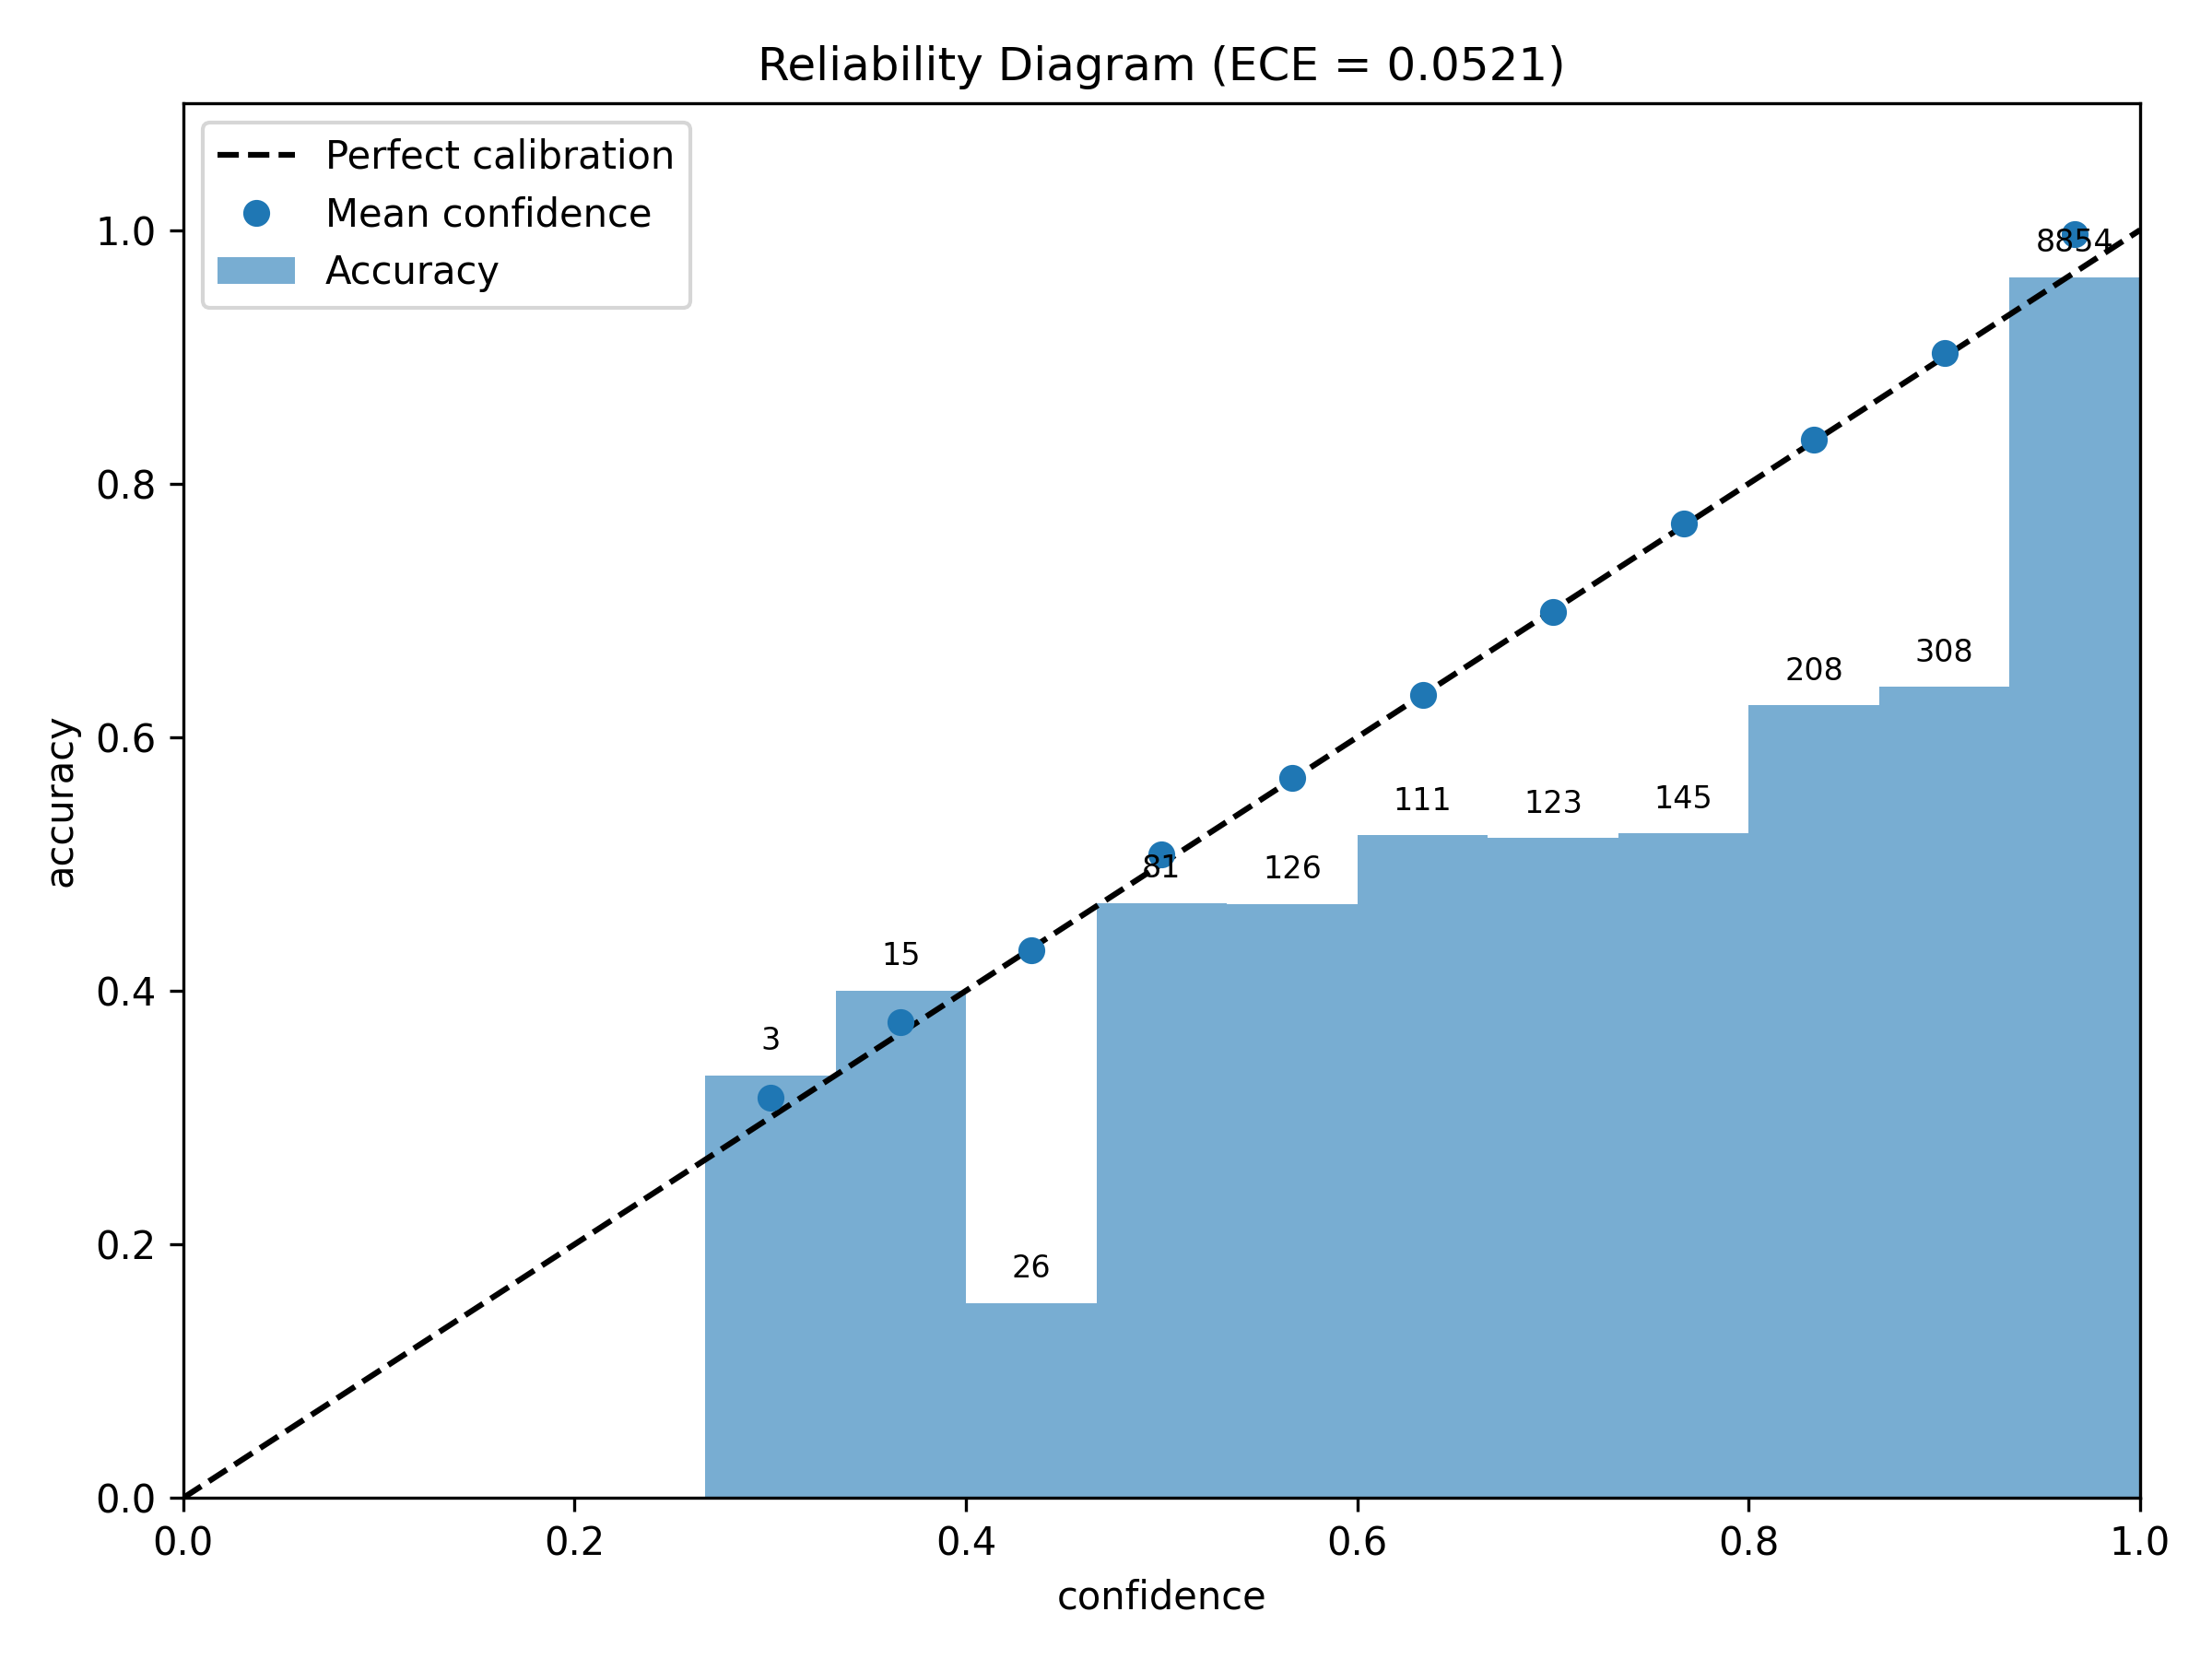
\includegraphics[width=0.47\linewidth]{../figures/reliability.png}\hfill
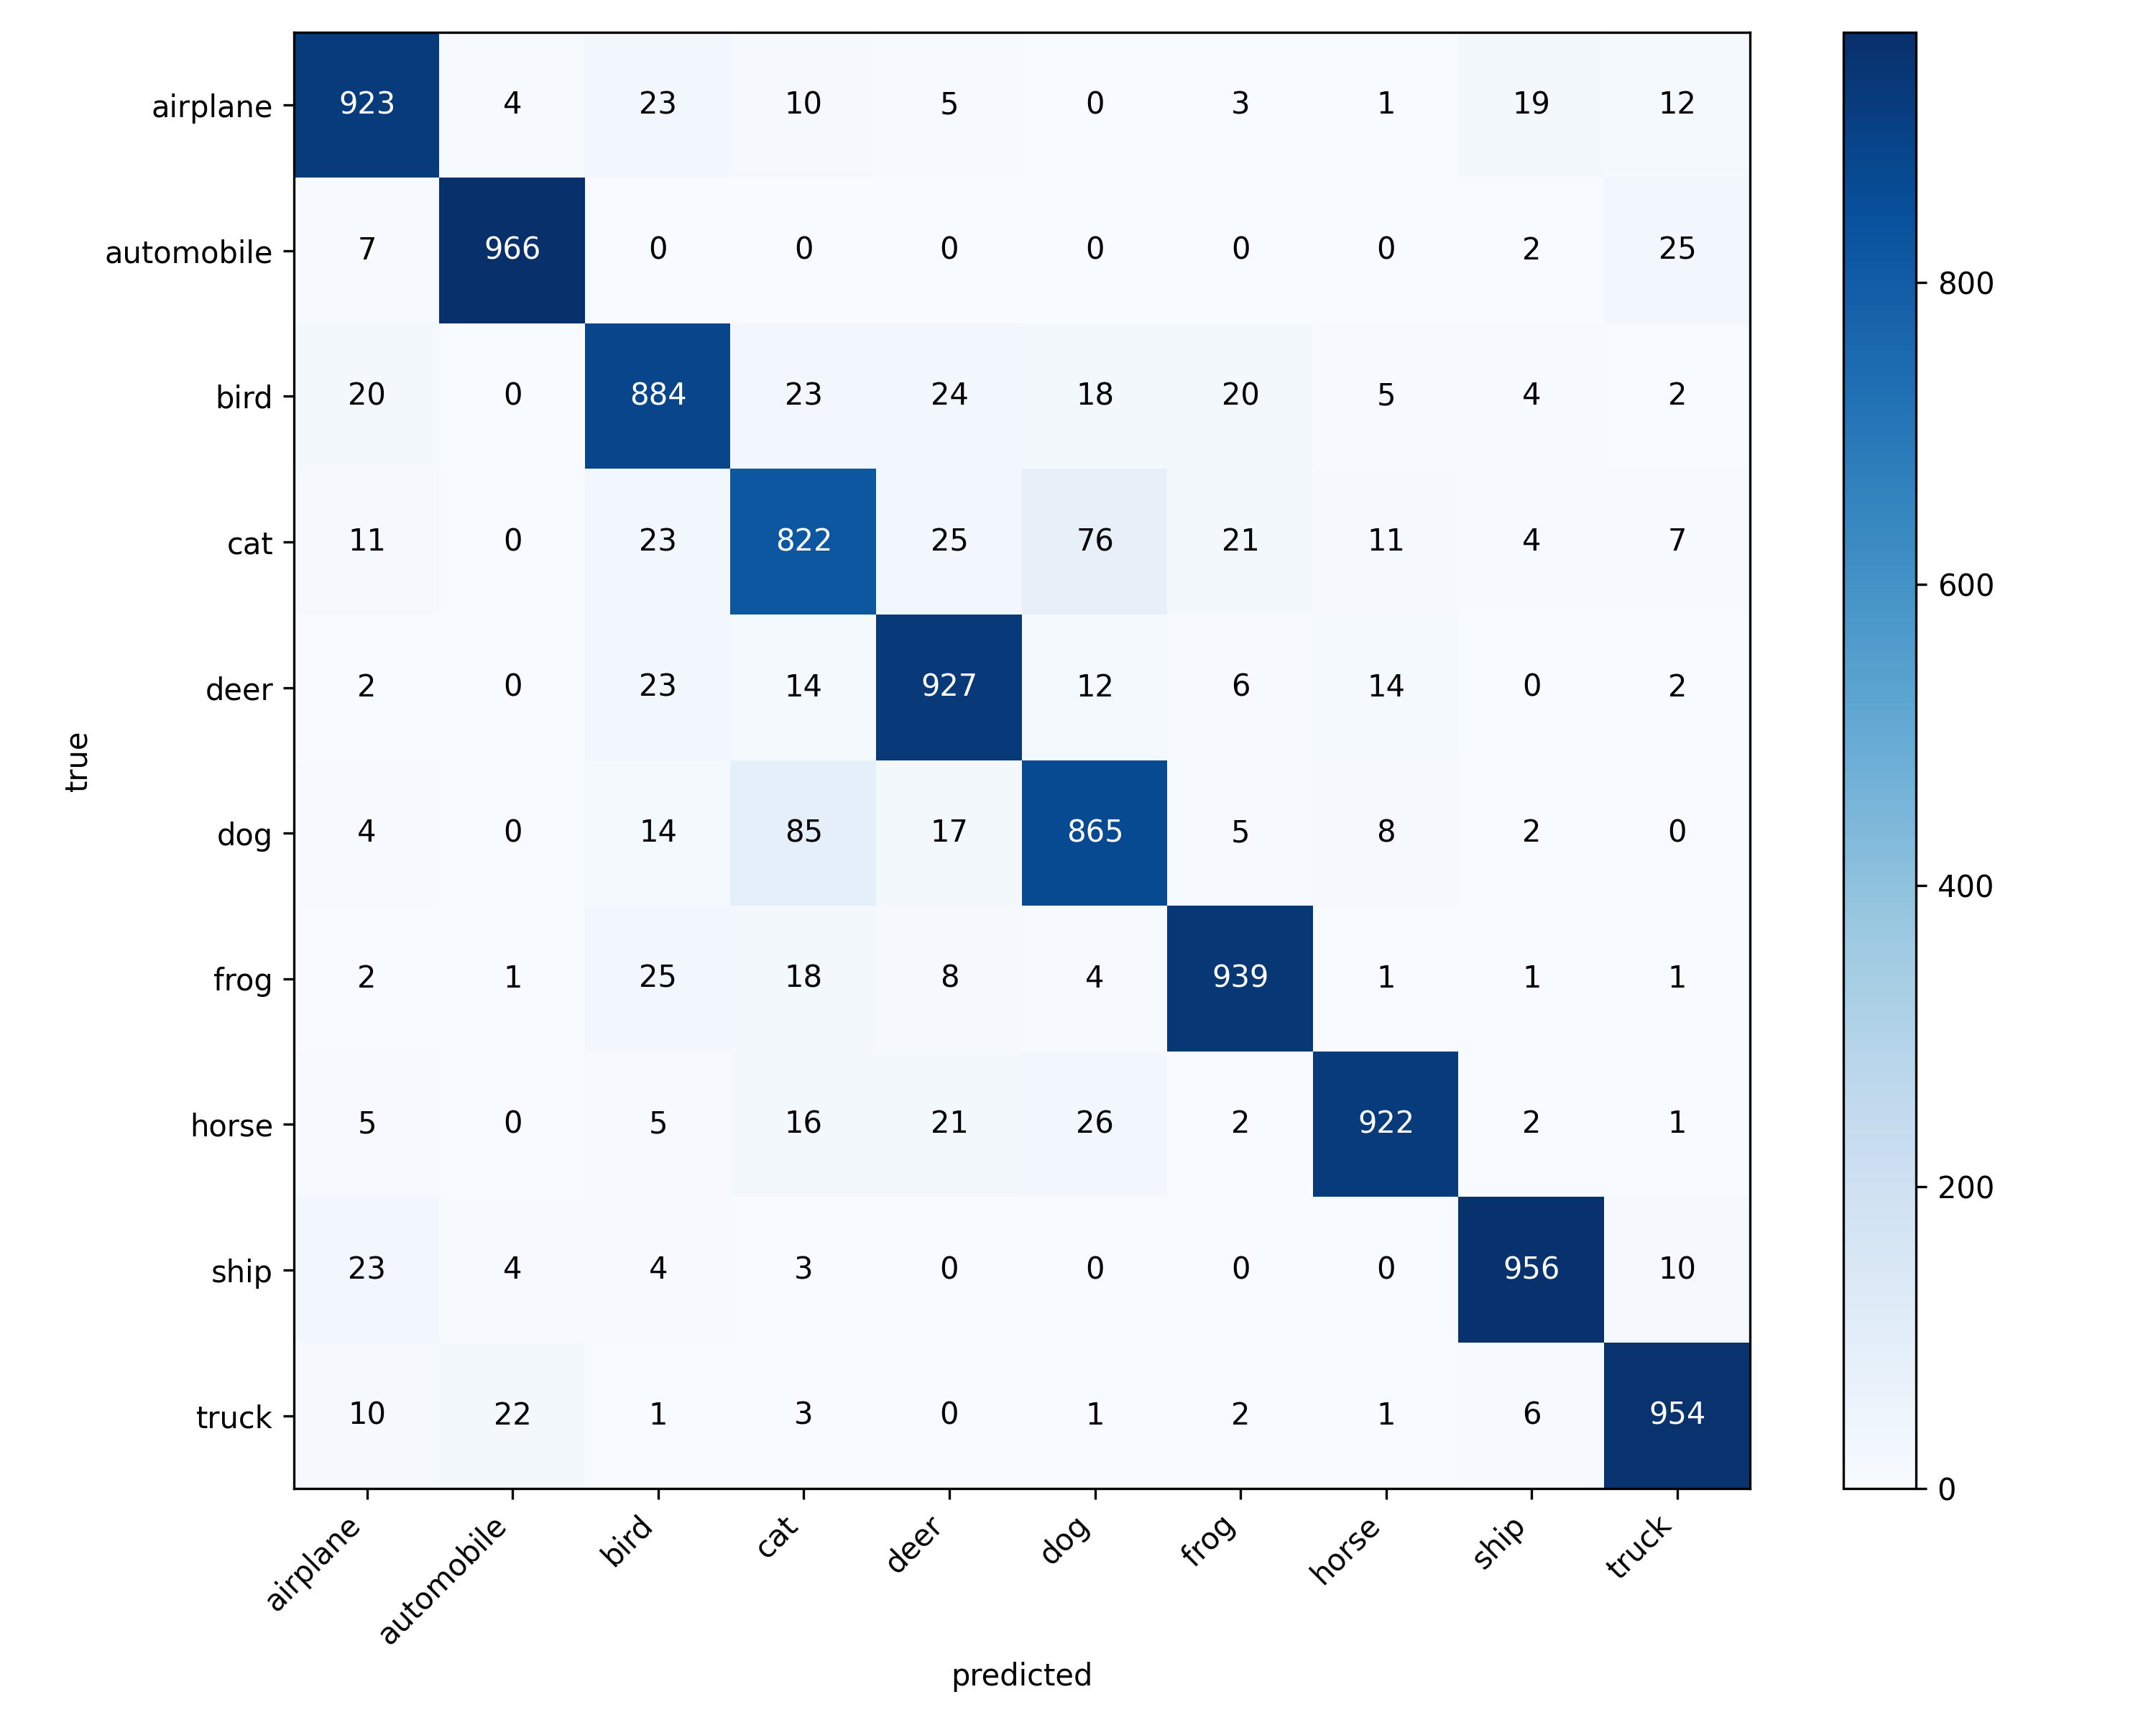
\includegraphics[width=0.47\linewidth]{../figures/confusion.png}
\end{center}

\begin{center}
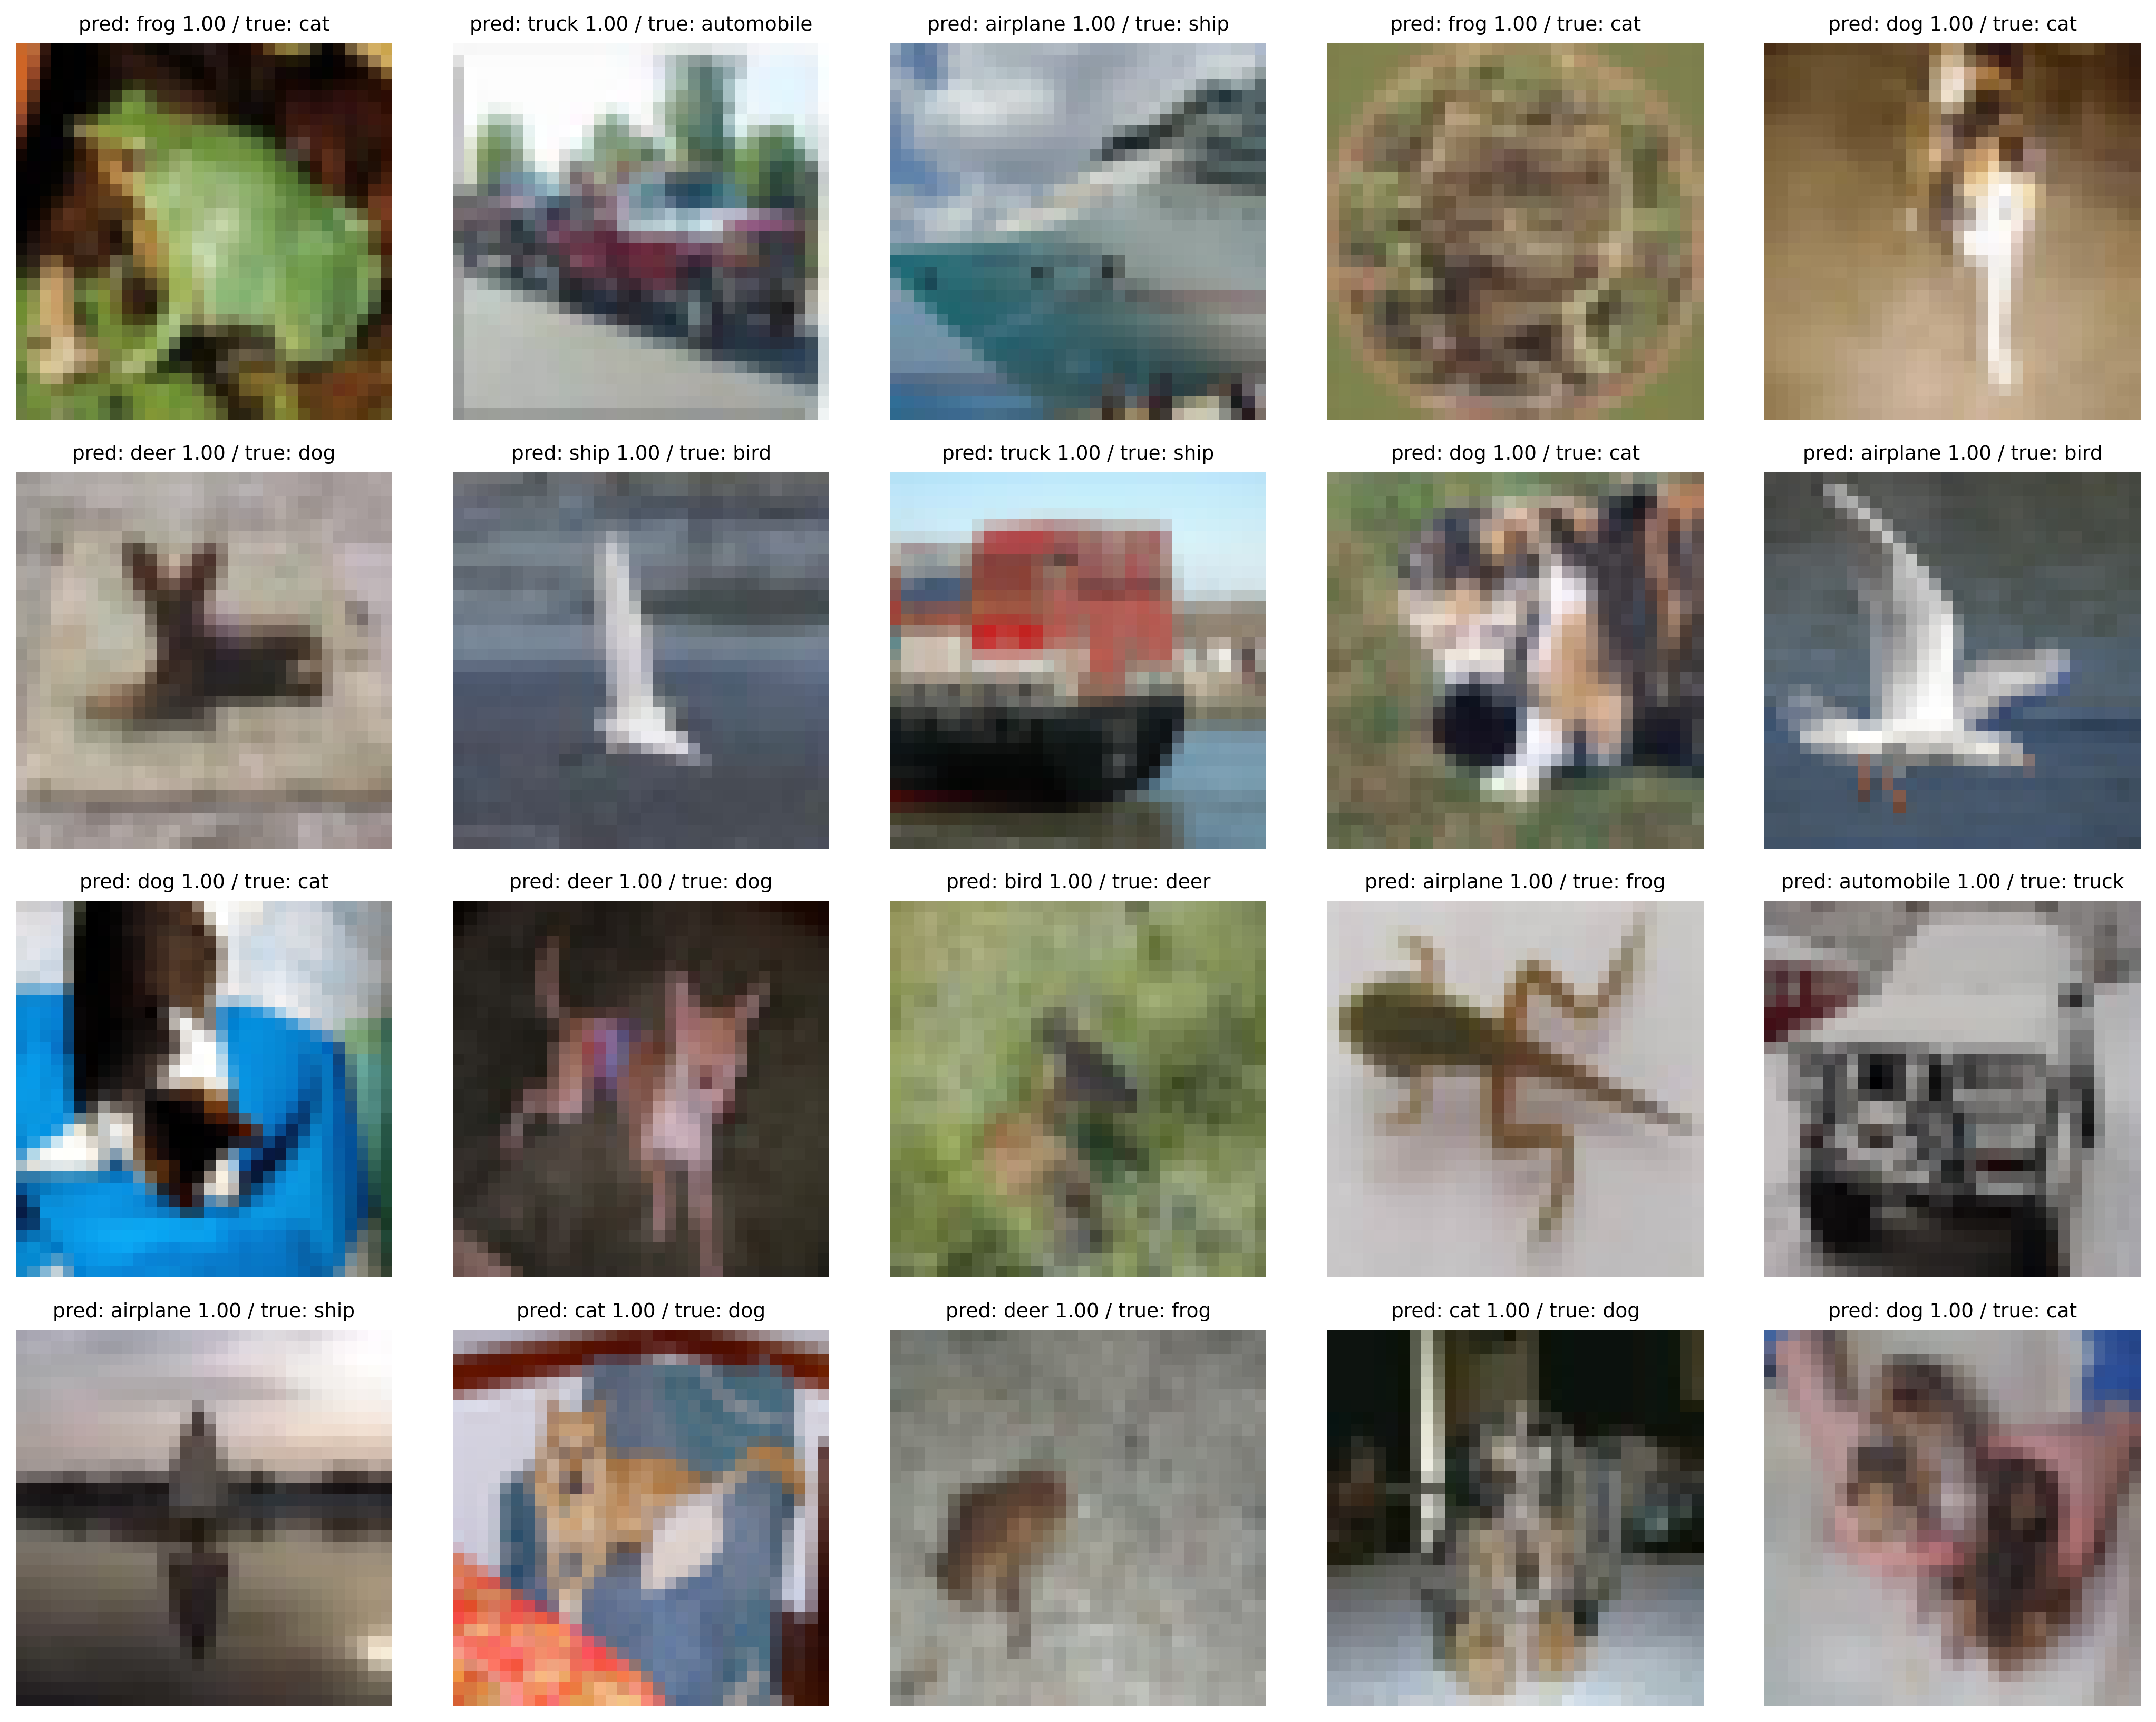
\includegraphics[width=0.85\linewidth]{../figures/confident_errors.png}

\small The 20 most confident wrong predictions (\file{docs/figures/confident\_errors.png}). Six are cat$\leftrightarrow$dog swaps, and the first is plausibly a label error in the dataset.
\end{center}

\subsection{Headline result}

\begin{repo}
\begin{center}
\begin{tabular}{@{}lrr@{}}
\toprule
model & test error, this repo & test error, paper\\
\midrule
ResNet-20 (trained on 50k, 64k iterations) & 8.42\% & 8.75\%\\
\bottomrule
\end{tabular}
\end{center}
Both are single runs. The paper's 5-run spread for ResNet-110 is $\pm0.16$ points, so a 0.33-point gap is ``matches the paper'', not ``beats it''. The test set was used once, after all choices had been made on the 45k/5k split.
\end{repo}

\subsection{Depth ablation: plain vs.\ residual}
\label{sec:ablation}

\begin{repo}[same recipe, 45k training images, seed 0]
\begin{center}
\begin{tabular}{@{}lrlrrr@{}}
\toprule
run & depth & type & train error & val error & test error\\
\midrule
ResNet-20 & 20 & residual & 0.52\% & 8.26\% & 9.29\%\\
plain-20 & 20 & plain & 0.88\% & 9.22\% & 9.77\%\\
ResNet-56 & 56 & residual & 0.08\% & 6.88\% & \textbf{7.92\%}\\
plain-56 & 56 & plain & \textbf{3.72\%} & 12.00\% & 12.94\%\\
\bottomrule
\end{tabular}
\end{center}
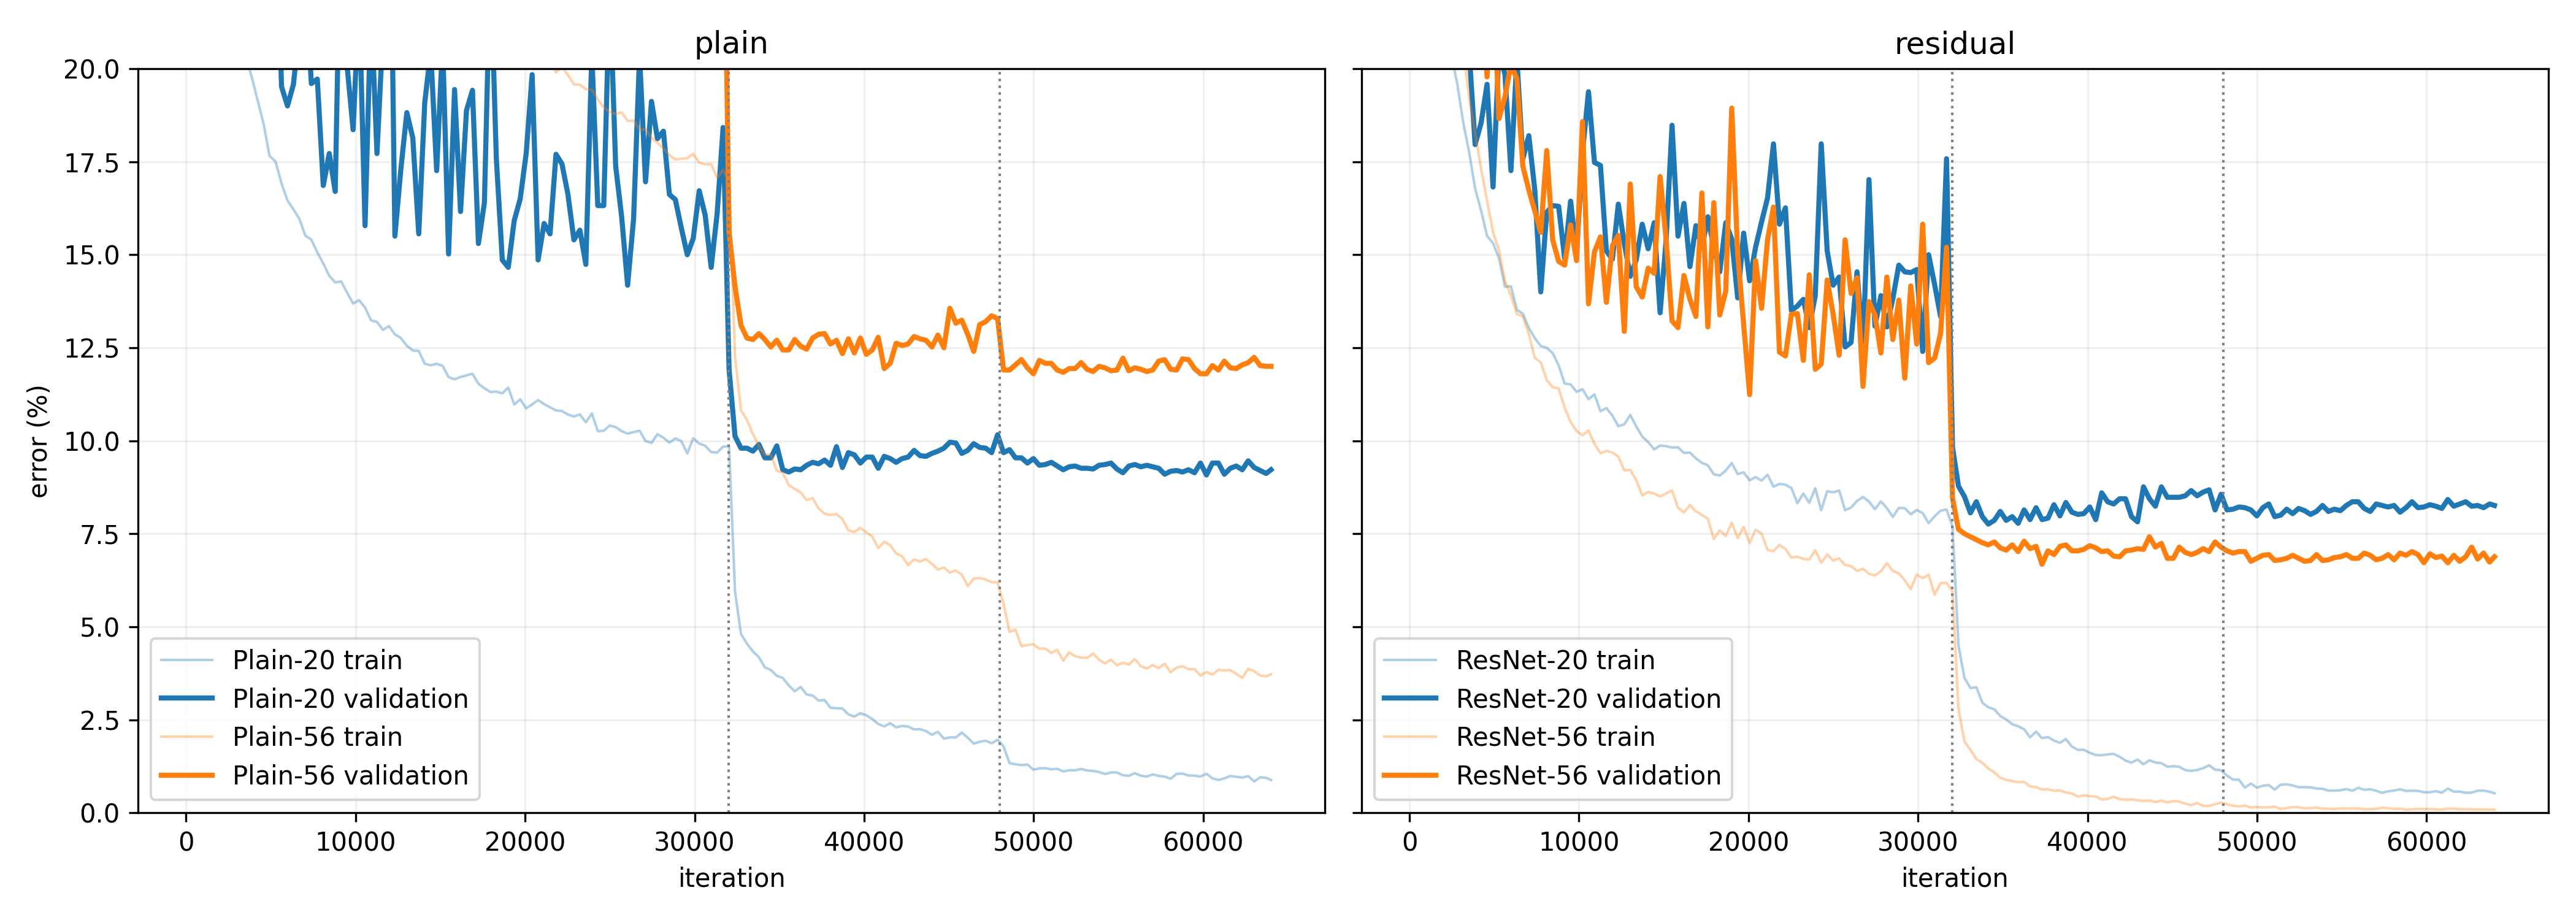
\includegraphics[width=\linewidth]{../figures/curves.png}
Going from 20 to 56 layers makes the plain network \emph{worse} (test $9.77\to12.94\%$), and its \emph{training} error rises too ($0.88\to3.72\%$). The deeper plain net is not overfitting. It fails to optimise, which is the degradation problem the paper set out to solve. The residual network improves with depth ($9.29\to7.92\%$). The two pairs have identical parameters and FLOPs (853{,}018 for both 56-layer nets), so the shortcut connection is the only difference. ResNet-56 takes 5{,}171\,s ($\approx86$ min) vs.\ 2{,}238\,s for ResNet-20 on the same GPU.
\end{repo}

\clearpage
\section{Inference and serving}
\label{sec:serving}

\begin{lstlisting}[firstnumber=11]
model = ResNetCIFAR(3)
load_checkpoint("model/resnet20.pt", model, None, device)
model.eval()
mean = np.load("model/pixel_mean_50k.npy")
...
@app.post("/predict")
async def predict_image(file: UploadFile):
    raw = await file.read()
    try:
        img = Image.open(BytesIO(raw)).convert("RGB")
    except UnidentifiedImageError:
        raise HTTPException(status_code=400,detail="Uploaded file is not a valid image")
    if img.size != (32,32):
        img = img.resize((32,32))
    arr = np.asarray(img)
    x = preprocess(arr,mean=mean).unsqueeze(0)
    with torch.no_grad():
        probs = torch.softmax(model(x),dim=1)
        values,indices = torch.topk(probs,3)
\end{lstlisting}

\begin{center}
\resizebox{\linewidth}{!}{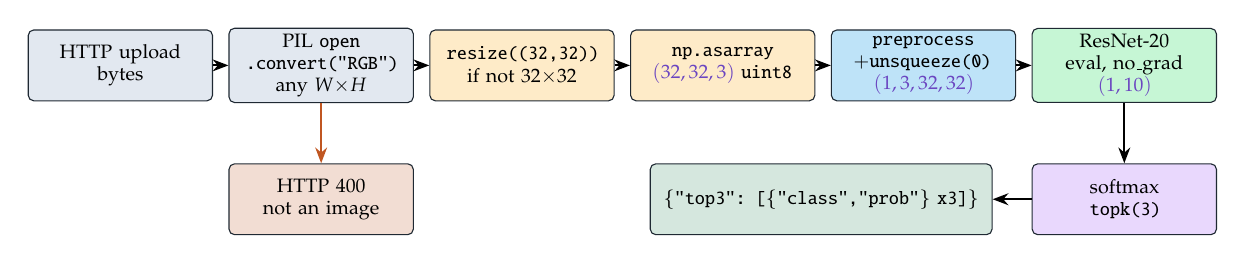
\begin{tikzpicture}[
  n/.style={draw=ink,rounded corners=2pt,fill=#1,font=\scriptsize,minimum height=0.9cm,align=center,inner sep=2pt,text width=2.2cm},
  n/.default=white, ar/.style={-{Stealth[length=2mm]},thick}]
  \node[n=cIn] (a) at (0,0) {HTTP upload\\bytes};
  \node[n=cIn] (b) at (2.55,0) {PIL \code{open}\\\code{.convert("RGB")}\\any $W{\times}H$};
  \node[n=cK] (c) at (5.1,0) {\code{resize((32,32))}\\if not $32{\times}32$};
  \node[n=cK] (d) at (7.65,0) {\code{np.asarray}\\\shp{32,32,3} \code{uint8}};
  \node[n=c16] (e) at (10.2,0) {\code{preprocess}\\$+$\code{unsqueeze(0)}\\\shp{1,3,32,32}};
  \node[n=c32] (f) at (12.75,0) {ResNet-20\\eval, no\_grad\\\shp{1,10}};
  \node[n=cG] (g) at (12.75,-1.7) {softmax\\\code{topk(3)}};
  \node[n=repo!20,text width=4.2cm] (h) at (8.9,-1.7) {\code{\{"top3": [\{"class","prob"\} x3]\}}};
  \node[n=warn!20] (err) at (2.55,-1.7) {HTTP 400\\not an image};
  \foreach \p/\q in {a/b,b/c,c/d,d/e,e/f,f/g,g/h} \draw[ar] (\p) -- (\q);
  \draw[ar,warn] (b) -- (err);
\end{tikzpicture}}
\end{center}

\begin{repo}[design points, each with a reason]
\begin{itemize}[nosep]
  \item \textbf{Same \code{preprocess} as training.} The service imports it from \file{cifar\_resnet/data.py} and uses the 50k mean that the final model was trained with. Training--serving skew in normalisation is the most common silent deployment bug, and sharing the function rules it out.
  \item \textbf{Loaded once, at import time}, in eval mode on CPU. \code{load\_checkpoint(..., None, ...)} skips the optimiser. The app prints the parameter count (269{,}722) and \code{model.training} (\code{False}) at start-up as a self-check.
  \item \textbf{Any image size is accepted} and resized to $32{\times}32$ with Pillow's default resampling filter. A large photo loses most of its detail, so predictions on it are less reliable than on CIFAR-like images. The README says so.
  \item \textbf{\code{.convert("RGB")}} turns grayscale, palette and RGBA images into three channels. An alpha channel is dropped, not composited.
  \item \textbf{Non-images} raise \code{UnidentifiedImageError} in PIL, which is mapped to HTTP 400 with a clear message instead of a 500.
  \item \textbf{Batch of one}: \code{unsqueeze(0)} adds $N=1$. This is safe only because BN is in eval mode. In train mode a batch of one would make $\sigma^2_c$ come from a single image.
  \item \textbf{\code{topk(probs, 3)}} returns the 3 largest values and their indices along the last axis, both \shp{1,3}, already sorted in decreasing order. The test \code{test\_valid\_image} checks the order and that \file{test0.png} is a cat.
\end{itemize}
\end{repo}

\begin{repo}[latency, from the README]
\begin{center}
\begin{tabular}{@{}lrr@{}}
\toprule
measurement (100 requests after 10 warm-up, $32{\times}32$ PNG) & p50 & p95\\
\midrule
native on Windows (uvicorn, CPU) & 3.9 ms & 7.0 ms\\
Docker Desktop on Windows (CPU) & 48 ms & 50 ms\\
model forward pass alone & 1.4 ms & --\\
\bottomrule
\end{tabular}
\end{center}
At $\approx40.6$M MACs, the forward pass takes about 1.4\,ms on a CPU. The rest of the native request time is HTTP, multipart parsing and PIL decoding. The extra $\approx44$\,ms in Docker Desktop is in the request path into the container, not in the model.
\end{repo}

\begin{repo}[container]
\file{Dockerfile}: \code{python:3.13-slim}, CPU-only \code{torch==2.14.1} from the PyTorch CPU index, then \file{requirements.txt} (FastAPI, NumPy, Pillow, python-multipart, uvicorn). It copies only \file{cifar\_resnet/}, \file{service/} and \file{model/} and runs \code{uvicorn service.app:app --host 0.0.0.0 --port 8000}. No torchvision is needed at serving time: \file{data.py} imports only \code{torch} and \code{numpy}.
\end{repo}

\clearpage
\appendix
\section{One-page cheat sheet}
\label{sec:cheat}

\subsection*{Forward shapes for a training batch ($N=128$)}
\begin{center}
\small
\begin{tabular}{@{}lll@{}}
\toprule
step & operation & shape\\
\midrule
raw & \code{data.data[idx]} & \shp{32,32,3} \code{uint8}\\
augment & pad 4 $\to$ \shp{40,40,3}, crop, flip & \shp{32,32,3} \code{uint8}\\
preprocess & $/255$, $-\mu$, permute & \shp{3,32,32} \code{float32}\\
batch & stack & \shp{128,3,32,32}\\
stem & conv $3{\to}16$ $(3{\times}3,S1,P1)$ + BN + ReLU & \shp{128,16,32,32}\\
stage 1 & 3 identity blocks & \shp{128,16,32,32}\\
stage 2 & block $16{\to}32$, $S2$ + 2 identity blocks & \shp{128,32,16,16}\\
stage 3 & block $32{\to}64$, $S2$ + 2 identity blocks & \shp{128,64,8,8}\\
GAP & mean over $8{\times}8$ & \shp{128,64,1,1}\\
flatten & & \shp{128,64}\\
linear & $pW\T+b$, $W$ \shp{10,64} & \shp{128,10}\\
loss & CE, mean & scalar\\
\bottomrule
\end{tabular}
\end{center}

\subsection*{Formulas}
\begin{align*}
&\text{conv output size:} && H_\text{out}=\lfloor (H+2P-K)/S\rfloor+1 \quad(32\to32 \text{ at } S{=}1,\; 32\to16 \text{ at } S{=}2)\\
&\text{conv params / MACs:} && C_\text{out}C_\text{in}K^2 \;/\; C_\text{out}C_\text{in}K^2H_\text{out}W_\text{out}\\
&\text{im2col:} && Y_\text{mat}=W_\text{mat}X_\text{col},\; (C_\text{out}\times C_\text{in}K^2)(C_\text{in}K^2\times H_\text{out}W_\text{out})\\
&\text{BN (train):} && y=\gamma\,(x-\mu_B)/\sqrt{\sigma_B^2+\varepsilon}+\beta, \text{ stats over } (N,H,W),\ \varepsilon=10^{-5}\\
&\text{BN running stats:} && r\leftarrow0.9\,r+0.1\,\text{stat}_B \quad(\text{unbiased variance})\\
&\text{block:} && y=\ReLU\big(\BN(\conv(\ReLU(\BN(\conv_S(x)))))+s(x)\big)\\
&\text{option-A shortcut:} && s(x)=\operatorname{pad}_\text{ch}\big(x[:,:,::2,::2]\big),\ (C_\text{out}-C_\text{in})/2 \text{ zero channels each side}\\
&\text{He init:} && \mathcal W\sim\mathcal N(0,\,2/(9C_\text{in}))\\
&\text{softmax, CE:} && s=\softmax(z),\quad \ell=\operatorname{logsumexp}(z)-z_y\\
&\text{logit gradient:} && G_Z=(S-Y_\text{onehot})/N\\
&\text{linear gradients:} && G_W=G_Z\T P,\quad G_b=\textstyle\sum_nG_Z[n],\quad G_P=G_ZW\\
&\text{BN gradient:} && G_a=\tfrac{\gamma}{m\sigma_\varepsilon}\big(mG_y-\textstyle\sum G_y-\hat a\sum G_y\hat a\big)\\
&\text{conv gradients:} && G_{W_\text{mat}}=\textstyle\sum_nG_{Y_\text{mat}}X_\text{col}\T,\quad G_{X_\text{col}}=W_\text{mat}\T G_{Y_\text{mat}}\ (\text{then col2im})\\
&\text{SGD:} && v\leftarrow0.9\,v+(\nabla\mathcal L+10^{-4}\theta),\quad \theta\leftarrow\theta-\eta v\\
&\text{schedule:} && \eta=0.1\ (t<32\text{k}),\ 0.01\ (t<48\text{k}),\ 0.001\ (t<64\text{k})\\
&\text{ECE:} && \textstyle\sum_b\frac{|\mathcal B_b|}{n}|\text{acc}(b)-\text{conf}(b)|,\ 15 \text{ bins}
\end{align*}

\subsection*{Numbers worth remembering}
\begin{center}
\small
\begin{tabular}{@{}ll@{\qquad}ll@{}}
\toprule
parameters (ResNet-20) & 269{,}722 & parameters (ResNet-56) & 853{,}018\\
share of params in stage 3 & 75\% & MACs / image & 40.6M\\
iterations / epoch (50k) & 391 & epochs (final run) & 164\\
training time (RTX 3050) & 36 min & test error & 8.42\% (paper 8.75\%)\\
ECE (15 bins) & 0.052 & mean confidence / accuracy & 0.968 / 0.916\\
CPU latency p50 (native) & 3.9 ms & forward pass alone & 1.4 ms\\
\bottomrule
\end{tabular}
\end{center}

\section{Things this project does \emph{not} contain}
\label{sec:notin}

So that future-me does not ``remember'' features that were never there:
\begin{itemize}[nosep]
  \item No $1{\times}1$ projection shortcuts (options B/C), no bottleneck blocks, no pre-activation blocks.
  \item No max-pooling, no dropout, no hidden fully connected layers, no softmax layer inside the model.
  \item No division by a pixel standard deviation, no colour jitter, no Cutout/Mixup, no label smoothing.
  \item No learning-rate warm-up (the paper uses one only for ResNet-110), no cosine schedule, no Nesterov momentum.
  \item No exclusion of BN/bias parameters from weight decay.
  \item No test-time augmentation: the test set is evaluated on single, original $32{\times}32$ views.
  \item No temperature scaling or other post-hoc calibration.
  \item No mixed precision, no multi-GPU, no data-loader workers, no per-epoch checkpointing.
\end{itemize}

\section{How this document was verified}

Every code excerpt is copied from the repository at commit \texttt{bf47649} (``README fixes before going public''). Every number labelled as measured was produced by loading \file{model/resnet20.pt} and \file{model/pixel\_mean\_50k.npy} into \code{ResNetCIFAR(3)} from \file{cifar\_resnet/model.py}, by reading \file{artifacts/logs/*.csv} and \file{artifacts/preds/final\_res20.npz}, or by counting parameters of the model classes. The forward and backward formulas were checked numerically against PyTorch (\cref{sec:forward}). This document was drafted with the help of an AI assistant from the repository's code and artifacts. The code it describes was written by hand.

\end{document}
